\documentclass[12pt]{article}

% Preamble
% Instead of a separeate file, all this must be in main.tex to make texlab function
% ---------------------------------------------------------------------------------
\renewcommand{\familydefault}{\sfdefault}  % switch default font to sans serif

\usepackage[utf8]{inputenc}
\usepackage{csquotes}

\usepackage[english]{babel}

\usepackage[a4paper,top=2.5cm,bottom=2.5cm,left=4cm,right=2.5cm,marginparwidth=1.75cm]{geometry}
\usepackage{parskip}

\usepackage{graphicx}
\usepackage[colorlinks=true, allcolors=black]{hyperref}

\usepackage{float}

\usepackage[acronym, nopostdot, style=list, nonumberlist, nogroupskip, toc]{glossaries}
% \setglossarypreamble[acronym]{\vspace*{-\baselineskip}}
\renewcommand{\glsnamefont}[1]{\textbf{#1}}

\makenoidxglossaries

\usepackage{array}
% https://tex.stackexchange.com/questions/12703/how-to-create-fixed-width-table-columns-with-text-raggedright-centered-raggedlef
\newcolumntype{L}[1]{>{\raggedright\let\newline\\\arraybackslash\hspace{0pt}}p{#1}}  % using p instead of m for top-allign
\newcolumntype{C}[1]{>{\centering\let\newline\\\arraybackslash\hspace{0pt}}m{#1}}
\newcolumntype{R}[1]{>{\raggedleft\let\newline\\\arraybackslash\hspace{0pt}}m{#1}}

\usepackage{booktabs}  % lists in tables
\newcommand{\tabitem}{~~\llap{\textbullet}~~}

% \usepackage{caption}
\usepackage[font=small]{caption}
\captionsetup{justification=raggedright}
\usepackage{subcaption}

% \usepackage{sectsty}  % sans serif headings the easy way
% \allsectionsfont{\sffamily}

\usepackage{titlesec}  % sans serif headings the hard way (but with exact HY style)
% \titleformat{<command>}[<shape>]{<format>}{<label>}{<sep>}{<before-code>}[<after-code>]
\titleformat{\section}{\large\sffamily\bfseries}{\thesection}{1em}{}
\titleformat{\subsection}{\normalsize\sffamily\bfseries}{\thesubsection}{1em}{}
\titleformat{\subsubsection}{\normalsize\sffamily}{\thesubsubsection}{1em}{}

\usepackage[style=apa6,uniquename=false]{biblatex}
\addbibresource{references.bib}

\usepackage[toc,page]{appendix}

\usepackage{pdfpages}  % pdf appendices

% Title page / abstract shenanigans
\usepackage{setspace}
\usepackage{tabularx}

\usepackage{makecell}
\usepackage{chngpage}
\usepackage{longtable}
\usepackage{cellspace}
\usepackage{booktabs}
\usepackage{multirow}
\usepackage{colortbl}
\usepackage{tablefootnote}
\setlength{\cellspacetoplimit}{6pt}
\setlength{\cellspacebottomlimit}{6pt}
\addparagraphcolumntypes{X}
\newcolumntype{?}{!{\vrule width 1.5pt}}
\newcommand{\Tstrut}{\rule{0pt}{2.2ex}}
\newcommand{\Bstrut}{\rule[-4.0ex]{0pt}{0pt}}
\newcommand{\TBstrut}{\Tstrut\Bstrut}
% \newcommand{\ra}[1]{\renewcommand{\arraystretch}{#1}}
\renewcommand{\arraystretch}{1.5}
\newcommand{\greyrule}{\arrayrulecolor{black!30}\midrule\arrayrulecolor{black}}
\newlength\tbspace
\setlength\tbspace{0.5cm}
% \newcolumntype{C}{c<{\hspace{\tbspace}}}%
% \newcolumntype{L}{l<{\hspace{\tbspace}}}%
% \usepackage{ragged2e}

% biblatex bibliography font
\renewcommand*{\bibfont}{\textrm}

% For appendix title settings
\usepackage{xpatch}
\xpretocmd{\appendixpagename}{\large\sffamily\bfseries}{}{}

% small sans serif page numbering
\usepackage{fancyhdr}
\fancypagestyle{plain}{
	\fancyhf{} % clear all header and footer fields
	\fancyfoot[C]{\sffamily\small\thepage}
	\renewcommand{\headrulewidth}{0pt}
	\renewcommand{\footrulewidth}{0pt}
}
\pagestyle{plain}

\raggedright
\linespread{1.25}

\newacronym{ttm}{TTM}{Helsinki region Travel Time Matrix}
\newacronym{ica}{ICA}{International Cartographic Association}
\newacronym{ykr}{YKR}{Community Structure Monitoring system}
\newacronym{gpu}{GPU}{Graphics Processing Unit}
\newacronym{cpu}{CPU}{Central Processing Unit}
\newacronym{gis}{GIS}{Geographic Information System}
\newacronym{hci}{HCI}{Human-Computer Interaction}
\newacronym{ue}{UE}{Usability Engineering}
\newacronym{ux}{UX}{User Experience}
\newacronym{ui}{UI}{User Interface}
\newacronym{os}{OS}{Operating System}
\newacronym{pc}{PC}{Personal Computer}
\newacronym{html}{HTML}{HyperText Markup Language}
\newacronym{http}{HTTP}{HyperText Transfer Protocol}
\newacronym{dom}{DOM}{Document Object Model}
\newacronym{css}{CSS}{Cascading Style Sheets}
\newacronym{api}{API}{Application Programming Interface}
\newacronym{ajax}{AJAX}{Asynchronous Javascript And Xml}
\newacronym{spa}{SPA}{Single-Page Application}
\newacronym{csc}{CSC}{Finnish IT Center for Science}
\newacronym{foss}{FOSS}{Free and Open Source Software}

\newcommand{\diagramwidth}{0.95\textwidth}
\newcommand{\posesscite}[1]{\citeauthor{#1}'s (\citeyear{#1})}
\newcommand{\presentacr}[1]{\acrlong{#1} (\acrshort{#1})}
\newcommand{\emphasizeacr}[1]{\textit{\acrlong{#1}} (\textit{\acrshort{#1}})}
\newcommand{\parenfig}[1]{(figure \ref{fig:#1})}
\newcommand{\parentab}[1]{(table \ref{tab:#1})}
\newcommand{\parenapp}[1]{(appendix \ref{appendix:#1})}
% ---------------------------------------------------------------------------------

\begin{document}

\pagenumbering{gobble}

\newgeometry{margin=2.5cm}  % same margins everywhere for title & abstract
\begin{center}{
    % \setstretch{1.0}  % more compact spacing
    \begin{figure}[H]
        \centering
        
\includegraphics[scale=0.4]{visual/other/helsinki_uni_logo.jpg}
    \end{figure}

    \bigskip
    \bigskip
    \bigskip
    \textbf{Master's thesis in Geography} \par
    \textbf{Geoinformatics} \par

    \bigskip
    \bigskip
    An interactive web map for visualizing travel time matrices -- A technical implementation and a user study

    \bigskip
    \bigskip
    Eemil Haapanen

    2024

    \vfill

    Supervisors: \\
    Professor Tuuli Toivonen \\
    PhD Christoph Fink \\
    ScD (Tech.) Pyry Kettunen \par
    \bigskip
    \bigskip
    \bigskip
    Master's Programme in Geography \par
    Faculty of Science \par
}
\end{center}

\begin{spacing}{1}
\setlength{\parskip}{4pt}

\textbf{Faculty:} Faculty of Science

\textbf{Degree programme:} Master's Programme in Geography

\textbf{Study track:} Geoinformatics

\textbf{Author:} Eemil Haapanen

\textbf{Title:} \mytitle

\textbf{Level:} Master's thesis, 30 credits

\textbf{Month and year:} April 2024  % TODO check

\textbf{Number of pages:} 86 + 11 appendices  % TODO check

\textbf{Keywords:}
Cartographic interaction,
Interactive map,
Map use,
User survey,
Web mapping,
Web map application.

\textbf{Supervisors:} Tuuli Toivonen (PhD), Christoph Fink (PhD), Pyry Kettunen (D.Sc. (Tech.))

\textbf{Where deposited:} University of Helsinki electronic theses library E-thesis/HELDA

\textbf{Additional information:} --

\textbf{Abstract:}
Cartographic interaction, the dialogue between a human and a map, is
a process enabling indispensable ways of reasoning with spatial information.
Interactive maps are digital applications,
increasingly often made with web technologies.
Studying and crafting cartographic interaction calls for
user-inclusive studies designed around interactive map use,
also necessitating the assessment of the rapidly evolving technologies enabling interactive maps.

This study combines the technology- and user-centric aspects of cartographic interaction.
I ask what the performance bottlenecks of a web map application are,
and how different web mapping libraries compare as a platform for real-time cartographic interaction.
I also ask how users interact with a highly interactive map interface,
and whether cartographic interaction changes the way they perceive the mapped phenomenon.

Developing a web map application,
a map interface to a massive dataset on spatial accessibility (the Helsinki region Travel Time Matrix),
is central to this study.
I answer my technology-centric questions by assessing the technological aspects of interactive maps
through the development process.
To answer my user-centric questions,
I carry out a user survey (n=31) by combining the web map application with an online questionnaire.

My results show that the geometrical complexity of data was the main factor limiting
map responsiveness, and that notable differences between web mapping libraries existed
in the context or real-time interaction.
Survey participants preferred to use the most dynamic mode of map interaction,
and perceived the mapped phenomenon differently depending on how they interacted with the map.

These results illustrate the dependence between map interface capabilities and technological design choices.
The results also support the wider call for more dynamic map interfaces,
indicating that real-time cartographic interaction can be a functional approach to exploring complex data.
As a whole, the results highlight the need for the ongoing study of both mapping technologies and map use
in order to discover and utilize the potential of cartographic interaction.

\newpage

\textbf{Tiedekunta:} Matemaattis-luonnontieteellinen tiedekunta

\textbf{Koulutusohjelma:} Maantieteen maisteriohjelma

\textbf{Opintosuunta:} Geoinformatiikka

\textbf{Tekijä:} Eemil Haapanen

\textbf{Tutkielman otsikko:}
Dynaaminen reaaliaikainen kartografinen interaktio matka-aikamatriisien tutkimisessa --
interaktiivisen web-karttasovelluksen kehitys sekä käyttäjäkysely

\textbf{Tutkielman taso:} Maisterintutkielma, 30 opintopistettä

\textbf{Kuukausi ja vuosi:} Huhtikuu 2024  % TODO check

\textbf{Sivumäärä:} 86 + 11 liitesivua  % TODO check

\textbf{Avainsanat:}
Interaktiivinen kartta,
Kartan käyttäminen,
Kartografinen vuorovaikutus,
Käyttäjäkysely,
Verkokarttasovellus.

\textbf{Ohjaajat:} Tuuli Toivonen (FT), Christoph Fink (FT), Pyry Kettunen (TkT)

\textbf{Säilytyspaikka:} Helsingin yliopiston avoin julkaisuaineisto E-thesis/HELDA

\textbf{Muita tietoja:} --

\textbf{Tiivistelmä:}
Kartografinen vuoraovaikutus, dialogi kartan ja sen käyttäjän välillä, mahdollistaa
korvaamattomia tapoja tutkia ja analysoida paikkatietoa.
Interaktiiviset kartat ovat digitaalisia sovelluksia,
joita toteutetaan yhä useammin verkkoteknologioilla.
Kartografisen vuorovaikutuksen tutkiminen ja hyödyntäminen vaatii
interaktiivisten karttojen käytön ympärille suunniteltuja osallistavia tutkimuksia,
sekä nopeasti kehittyvien karttateknologioiden arviointia.

Tämä tutkimus yhdistää kartografisen vuorovaikutuksen teknologia- ja käyttäjäkeskeiset näkökulmat.
Kysyn, mitkä tekijät rajoittavat verkkokartta-sovelluksen suorituskyä,
ja miten erilaiset verkkokarttakirjastot toimivat alustana reaaliaikaiselle kartografiselle vuorovaikutukselle.
Kysyn myös, miten käyttäjät käyttävät interaktiivista karttakäyttöliittymää,
ja muuttaako kartografinen vuorovaikutus tapaa, jolla kartan käyttäjä hahmottaa kartoitetun ilmiön.

Keskeinen osa tuskimusta on kehittää interaktiivinen verkkokarttasovellus
massiiviselle paikkatietoaineistolle spatiaalisesta saavutettavuudesta (Pääkaupunkiseudun matka-aikamatriisi).
Vastaan teknologiakeskeisiin kysymyksiini tämän kehitysprosessin kautta.
Käyttäjäkeskeisiin kysymyksiini vastaan suorittamalla käyttäjäkyselyn (n=31),
jossa tutkin verkkokarttasovelluksen käyttöä verkkokyselyllä.

Tulokseni osoittavat, että visualisoitavan aineiston geometrinen monimutkaisuus
oli kartan suorituskyvyn päärajoite, ja että verkkokartta-kirjastojen välillä oli
huomattavia eroja reaaliaikaisen vuorovaikutuksen kontekstissa.
Kyselyyn osallistujat suosivat karttakäyttöliittymän dynaamisinta vuorovaikutustapaa,
ja hahmottivat kartoitetun ilmiön eri tavalla riippuen siitä, kuinka he käyttivät karttaa.

Nämä tulokset havainnollistavat riippuvuutta kartta-käyttöliittymien ominaisuuksien
ja teknologisten suunnitteluratkaisujen välillä.
Tulokset myös tukevat laajalti tiedostettua tarvetta dynaamisemmille karttakäyttöliittymiille,
osoittaen, että reaaliaikainen kartografinen vuorovaikutus voi olla toimiva lähestymistapa suurtenkin
paikkatietoaineistojen tutkimiseen.
Kokonaisuutena tulokset korostavat tarvetta
sekä karttateknologioiden että karttojen käytön kokonaisvaltaiseen tutkimiseen,
jotta interaktiivisten karttojen potentiaalia voitaisiin hyödyntää.

\end{spacing}

% \newpage

\tableofcontents

\restoregeometry  % back to initially specified geometry

\cleardoublepage
\pagenumbering{roman}  % TODO use arabic everywhere?

\newpage
\addcontentsline{toc}{section}{List of Figures}
\listoffigures
\newpage
\addcontentsline{toc}{section}{List of Tables}
\listoftables
\newpage
% \addcontentsline{toc}{section}{List of Acronyms}
\printnoidxglossary[type=acronym, title={List of Acronyms}]

\cleardoublepage
\pagenumbering{arabic}

\rmfamily  % switch to roman (serif) base font for rest of the thesis

\section{Introduction}
% Start with cartography instead? (kra2021)

% Cartography
% importance: recent developments, data, revealing patterns. See also \textcite{kra2021}.

% Accessibility shortly
% Accessibility from a cartographical angle
% challenges in presenting

Maps are ubiquitous and essential to human civilization.
In addition to depicting our geographical surroundings,
they help us reveal and understand new patterns and phenomena,
and to gain insights from information
that would otherwise be hard or impossible to interpret \parencite{mac2004}.
Currently, we live in a world that is in a state of rapid and
alarming change \parencite{un2023},
but where information is available in an unprecedented abundance
\parencite{rob2017a, un2023}.
Acknowledged as one of the most pressing issues of the ongoing decade,
efficiently harnessing this data is a requirement
for the well-being of the entire planet \parencite{un2020}.
As the quantity of data grows
and understanding it becomes more and more demanding,
the relevance of maps and cartography is only increasing.
Maps, mapping technologies and cartography are essential,
as they can provide unique ways to synthesize and make sense of complex data,
of which there is no shortage \parencite{kra2021}.
% To summarize, any means that allow us to make sense of an overflow of information are vital,
% and maps and cartography certainly are such means.
% and it is no coincidence that \textcite{kra2021}

From this perspective,
interactive maps, more specifically digital interactive map applications,
can be seen as especially vital.
% Why interactive maps good
As opposed to approaching maps solely as communicative devices or representations
that are made to be passively read,
the concept of cartographic interaction redistributes the agency in how maps work.
Not only a reader, the map user has the capability of actively manipulating the map,
and the map, in turn, has the capability of adapting to the manipulation \parencite{eds2008}.
From such user-map exchanges emerges a dialogue:
A process where, in addition to the map user altering the map,
the map affects the user as they perceive and evaluate the results of their map manipulation
\parencite{rot2011}.
Such blend of simultaneous mapmaking and -reading
is considered highly conductive to analytical thinking and reasoning
with spatial data,
enabling new ways to solve novel and increasingly complex problems
\parencite{rob2017b, and2010}.
In addition to consciously analytical expert use,
interactive maps and accompanying technologies have found their place
in the everyday lives of most.
Cartographic interaction, for example in the form of online and mobile map applications,
can in this sense be seen to facilitate the access to spatial information
for the many rather than the few \parencite{mei2019}.

While cartography has long been considered a highly multidisciplinary science,
understanding and crafting cartographic interaction necessitates an even
more diverse set of research themes, questions and methods.
The transition from the map reader to the map user
introduces the cognitive process of map use in addition to map reading
\parencite{mac2015, liu2010},
and requires envisioning the map as an interface in addition to a representation
\parencite{rot2013b}.
Gaining insight on how the map interface is used, perceived and reasoned with
means including the user into the cartographic process,
and calls for studies designed around map use specifically as enabled by cartographic interaction
\parencite{rot2017}.

At a technological level,
the notion of interactive maps as digital applications relates maps to software.
Often, this software more particularly refers to web applications:
The web has for a while been considered the de-facto software platform \parencite{tai2017, mik2019},
and a clear majority of interactive maps are being made for the web \parencite{vee2017}.
This means that the tools of the mapmaker
increasingly resemble those of a web developer \parencite{rot2021}.
The assessment of these tools from a cartographic perspective is
an effort regarded as both necessary and topical:
Necessary since software defines the technological possibilities and limits
of cartographic interaction,
and topical due to the rapid pace of technological innovation
and the equally fast increase of the requirements placed upon map interfaces
\parencite{rot2014, rot2021}.

In this study I approach cartographic interaction from two points of view,
with two main goals.
From a technology-centric perspective,
I aim to assess the tradeoffs, limitations and technologies to be considered when
striving for an interactive, dynamic and responsive web map interface to complex data.
% I aim to find out how web-based cartographic interaction can be utilized in exploring
% massive geospatial data.
From a user-centric perspective,
my goal is to study how
map users utilize a highly interactive map interface
and how they perceive the mapped phenomenon
through cartographic interaction.


Both my goals revolve around developing an interactive web map application --
a map interface for exploring the \presentacr{ttm} \parencite{fin2023}.
In short, the \acrshort{ttm} is a large dataset on spatial accessibility,
containing travel times for
over 175 million unique routes by a multitude of travel modes
in the Helsinki region, southern Finland.
Functionally speaking, the goal of the map interface is to enable
a user to explore travel times to all locations included in the dataset,
by all travel modes.
Considering the scale of the dataset,
a dynamic, real-time approach to interaction is necessary
if any meaningful portion of the data is to be explored.
More descriptively, the interface should allow for flexible and
responsive (dynamic) interaction exchanges that happen with as little as possible delay
perceived by the user (in real-time).
% The main design factor
In the context of my technology-centric goal,
the development process and the map application are the framework
allowing me to study the technological aspects interactive maps.
Considering my user-centric goal,
the development process outputs an interactive map application
to be used in studying how such an interface is used and understood by map users.

I further delineate the focus of my work with the following research questions:

\begin{itemize}
	\item Considering dynamic real-time interaction,
	what are the performance bottlenecks of
	a web-based interactive map,
	and what data preprocessing and simplifying methods
	are needed to overcome them?
	\item What differences are there between web mapping libraries
	when used as a platform for dynamic real-time cartographic interaction?
	\item Which types of user-map interaction do map users utilize
	in different types of map usage scenarios?
	\item Does dynamic real-time interaction with a map change
	the map user's perception of the mapped phenomenon? If it does, how?
\end{itemize}

The first two research questions relate tightly to the development process.
I answer the first question by assessing different approaches to
preprocessing and simplifying a complex dataset (the TTM),
the goal being to find what characteristics of the data
limit the responsiveness of the map interface the most (are the performance bottlenecks),
and what kind of data preprocessing is needed to achieve real-time interaction with the map.
To answer the second question,
I assess how different web mapping libraries compare when used in the implementation
of a highly interactive web map application.

The latter two research questions switch the focus to user-map interaction.
I answer these questions by carrying out a user survey
where I combine the interactive web map application with
a semi-structured online questionnaire.
The questionnaire employs a task-based design
to allow for gaining insight on different scenarios of map use
and to see whether the way the user interacts with the map
affects how they perceive the mapped phenomenon.
In addition, I supplement the task-based structured portion of the questionnaire
with unstructured questions to gain qualitative insight on map use and perception.

This thesis explores the theory and technology
needed to study cartographic interaction and to craft interactive web map applications,
also concisely acknowledging the implications that the mapped phenomenon,
i.e. spatial accessibility, introduces to crafting a map interface.
Applying all this to practice, this thesis documents the technical implementation
of a web-map application and the survey process on map use.
Finally, this thesis relates the results to the wider scientific discussion
in the context of modern-day web-mapping, interactive cartography and geovisual analytics. 


% % ------------------------
% When describing the presentation I use the word system.
% This is because crafting such a presentation
% requires the mapmaker to make much more than a map --
% It means designing, implementing and optimizing
% a whole that consists of multiple components.
% These components all have their distinct purposes yet must function together
% to meet the requirements placed upon the whole.
% \begin{itemize}
% 	\item Preprocessing the dataset (the \acrshort{ttm}) to a mappable format,
% 	and simplifying it to enable its interactive exploration over the internet
% 	\item A solution for storing and serving the data, i.e. the backend
% 	\item A web application for interactively presenting the data, i.e. the frontend
% \end{itemize}

% The ultimate purpose of the entire system is to enable a map.
% The map, in turn, has a goal of conveying information;
% it is a representation of the mapped phenomenon.
% However, studying how the map works,
% not as a piece of technology but as a representation,
% is impossible based on a technical implementation alone.

% My second research goal is to understand how
% this particular representation of accessibility conveys information.
% I aim to find out how the map user understands the map,
% and how they use cartographic interaction to explore the mapped phenomenon.
% % ------------------------

% % This thesis applies all this to accessibility
% In this thesis I relate cartography to accessibility.
% When referring to accessibility,
% I more specifically mean spatial accessibility, that is,
% the ease of reaching valued destinations in physical space \parencite{lev2020}.
% Understanding accessibility is important,
% as the phenomenon is deeply interlinked in our society.
% Accessibility affects the choices and experiences of individuals \parencite{kwa1998, kwa2003}
% as well as the planning and governance processes
% of much larger entities such as cities \parencite{cur2010, low2015}.
% It is also directly linked to significant and ongoing issues such as
% urban well-being \parencite{zha2011},
% equity and justice \parencite{per2017, che2020}
% and sustainable transport and mobility \parencite{son2017, mah2019}.
% In general, research in accessibility helps us understand
% how societal systems and phenomena function
% in different scales and timeframes, and from different points of view.

% % difficulty in defining and measuring access
% However, analysing or even comprehending accessibility
% in a holistic manner is not simple.
% While a common starting point for defining the term is, quite concisely,
% \enquote{potential of opportunities for interaction} \parencite{han1959},  % define interaction in more detail?
% more precise definitions and measurements can be constructed in countless ways
% depending on the factors deemed impactful to that potential
% \parencite{pap2016}.
% For example, even with a simple consideration of travel distance as a measure of access,
% including all the different things this access can be measured in relation to
% would make the amount of variations, i.e. different \enquote{accessibilities},
% to measure grow exponentially \parencite{lev2020}.
% In addition, accessibility is inherently tied not only to location
% but also time \parencite{jar2018},
% meaning every place in every time has a level of access
% in relation to every other place.

% % hard to visualise too
% Because of its composite and dynamic nature,
% constructing representative cartographic visualizations of accessibility is difficult.
% Accessibility visualizations are often constrained
% to displaying access in relation to
% a limited number of pre-selected places (for example \textcite{wei2018}),
% or composing an accessibility index
% that can be calculated and mapped for all locations,
% in relation to potentially many different things and locations
% (for example \textcite{kim2019}).
% However, more complex accessibility measures tend to lead to
% less usable presentations \parencite{te2014},
% while mapping more simple measures could lead to an influx of variations to present.
% For example, separating different travel modes, times of day or target locations
% would multiply the amount of visualizations needed to present accessibility.

% % Not only methodological but also a cartographical challenge 
% % something that is not a physical feature nor an easily explainable variable
% % ----------------------------------------
% % general stuff about cartography - what types of phenomena / maps
% % how is accessibility different?
% % ----------------------------------------
% % Why is visualising access important?
% % This could be before the preceding chapter too?
% % Leave something for background chapter too

% % how interactivity benefits accessibility visualisation (because of how accesibility is)
% Even if visualizing every aspect of accessibility
% from everywhere to everywhere is impossible,
% careful consideration and implementation
% of the cartographic methods we have at our disposal might get us closer.
% Interactive cartography could be one approach with great potential.
% After all, a key principle of interactivity in map presentations is
% the map user's ability to change the content of the map \parencite{rot2013b}.
% For visualizing accessibility this could mean, for example,
% interactive selection of location or travel mode instead of
% a static accessibility index that, to a varying extent,
% tries to account for everything.
% Scientific literature on the topic seems to support the idea of
% interactivity in accessibility visualization,
% even indicating a need for such presentations.
% In a study focusing on the usability of
% different accessibility instruments and visualizations,  % accessibility instrument
% \textcite{te2014} highlight the importance of
% real-time interactivity between the map and the map user.
% \textcite{but2018} state that for maps to efficiently communicate accessibility,
% they should be as flexible and dynamic as possible.
% However, \textcite{but2018} also note that
% these qualities are often missing in accessibility visualizations.
% Along the same lines,
% \textcite{paj2021} find modern accessibility visualizations often complicated,
% and lacking in interactivity and flexibility.

% % research questions
% % Communicating accessibility instead of analyzing it
% % How to utilize interactive mapping in communicating accessibility

% In this thesis I focus on
% how cartographic interaction can be utilized in presenting accessibility.
% My research has two main goals.
% The first is to produce an interactive accessibility visualization --
% I develop a system for interactively presenting a massive accessibility dataset,
% the \acrlong{ttm} (\acrshort{ttm}) \parencite{fin2023},
% on the web.  % TODO introduce the matrix somewhere, maybe here?
% The \acrshort{ttm} is a dataset containing travel times for
% over a 175 million unique routes, by a multitude of travel modes,
% in the Helsinki region, southern Finland.
% The sheer volume and detail of the dataset allows for endless options
% in its presentation, and, from the perspective of this thesis,
% a real opportunity and a need to take advantage of interactivity in visualizing it.
% By using cartographic interaction
% I aim to extend the multi-location and multi-modal nature of the dataset
% to its presentation.
% The map user should be able to explore, on a map,
% travel times to all locations included in the dataset,
% by all travel modes.
% However, interaction alone does not yet enable this.
% Considering the number of different combinations of location and travel mode,
% interaction with the map must happen in real-time,
% i.e. with instant visual feedback.
% Only with this quality is it possible for the map user to
% explore any meaningful portion of the \acrshort{ttm}
% in a reasonable amount of time.

% When describing the presentation I use the word system.
% This is because crafting such a presentation
% requires the mapmaker to make much more than a map --
% It means designing, implementing and optimizing
% a whole that consists of multiple components.
% These components all have their distinct purposes yet must function together
% to meet the requirements placed upon the whole.
% While being a map first and foremost, the complete system
% requires implementing all the following components:
% \begin{itemize}
% 	\item Preprocessing the dataset (the \acrshort{ttm}) to a mappable format,
% 	and simplifying it to enable its interactive exploration over the internet
% 	\item A solution for storing and serving the data, i.e. the backend
% 	\item A web application for interactively presenting the data, i.e. the frontend
% \end{itemize}

% The ultimate purpose of the entire system is to enable a map.
% The map, in turn, has a goal of conveying information;
% it is a representation of the mapped phenomenon.
% However, studying how the map works,
% not as a piece of technology but as a representation,
% is impossible based on a technical implementation alone.

% My second research goal is to understand how
% this particular representation of accessibility conveys information.
% I aim to find out how the map user understands the map,
% and how they use cartographic interaction to explore the mapped phenomenon.


% My research questions reflect the goals of this study.  % TODO
% The first goal, being the interactive map presentation,
% necessitates research on the options and tools
% needed in its implementation.
% The way I approach this research is through qualities
% that the resulting system should have.
% As real-time interactivity is a priority of the map presentation,
% the performance of the system,
% i.e. minimizing the latency between
% the software receiving input and displaying results of said input,
% is one key aspect to consider.
% Just as essential is the visual quality of the map
% and the intuitiveness of its use.
% % discussion perhaps?
% % I also stress the importance of
% % \textit{how} the system is designed and developed.
% % If the software cannot be understood or maintained,
% % it has little real value,
% % no matter how performant the implementation or how elegant its user interface.

% % With these qualities and the aforementioned components of the system in mind,
% % I structrure the research.

% % While the resulting system, as a whole, should have all these qualities,
% % each part of the system is ultimately its own entity.
% % This is important to keep in mind when forming research questions,
% % as some qualities are naturally more or less important depending on the component.
% % For example,
% % visual quality has little to do with backend implementation.

% Considering the aforementioned components
% and the desired qualities of the system,
% my research questions in regard to its implementation are:

% \begin{itemize}
% 	\item Considering rapid real-time interaction,
% 	what are the performance bottlenecks of
% 	a web-based interactive map,
% 	and what data preprocessing and simplifying approaches
% 	are needed to overcome them?
% 	\item What differences are there between web mapping libraries
% 	when used as a platform for rapid real-time cartographic interaction?
% \end{itemize}  % TODO maybe list approaches -> which is best? Geometry simplification etc...

% % TODO move following to study design?

% % I answer the first question by evaluating approaches based on three criteria:
% % \begin{enumerate}
% % 	\item the impact on file size,
% % 	and thus on the time needed to transfer the files over the internet
% % 	\item the impact on rendering speed of the map when mapping the data
% % 	\item the impact on the visual detail of data,
% % 	i.e. how much information is lost
% % \end{enumerate}

% % File sizes can be compared quantitatively.
% % When evaluating rendering speed,
% % I combine quantitative tests of rendering speed with
% % my own qualitative assessment of the rendering performance when using the map.
% % I evaluate the visual detail by my own qualitative assessment.

% % I choose the most efficient solution for
% % storing and serving the data based on a qualitative assessment of
% % the available options. I define efficient as:
% % \begin{enumerate}
% % 	\item Introducing the least possible performance overhead
% % 	\item Introducing the least possible technical complexity
% % \end{enumerate}

% % I base my comparison of web mapping libraries on three criteria:
% % \begin{enumerate}
% % 	\item Visual quality of the map
% % 	\item Responsiveness of the map
% % 	\item User interface capabilities for interacting with the map
% % \end{enumerate}

% % The first two criteria I evaluate qualitatively. The third criteria, while an inherent quality of a mapping-library, Is that too ultimately my own view.  % TODO

% In order to gain insight on how the map functions as an interface and a representation,
% I focus on how people work with and understand the map.
% My research questions are:  % TODO?

% \begin{itemize}
% 	\item Which types of interaction available in the map do people use
% 	in different types of usage scenarios?
% 	\item Does rapid real-time interaction with the map change
% 	the map user's perception of the mapped phenomenon? If it does, how?
% \end{itemize}

% To answer these questions, user perspective is of course required.
% Thus, I carry out a survey
% where I combine the interactive map presentation with
% a semi-structured online questionnaire.

% In addition to directly addressing the aforementioned research questions,
% the survey has an important role in validating the map presentation.
% The complete system can be judged by
% how, and if, it works when used by real people.

% % In this sense, the survey brings additional weight to
% % the results of the technical research questions
% % as well as other choices related to the implementation of the map.

% % and whether map interaction impacts their understanding of the mapped phenomenon.

% % their order of importance depends on the part of the system being considered.
% % I value them differently depending on the  system With these qualities in mind I can then be applied to 
% % the parts of the system
% % that are visible to the user, i.e. the map application, or frontend.
% % Thus, the research questions I ask are:
% % at all stages of the implementation.
% % In regard to the performance of the map application,
% % there are three main components stages at which implementation decisions must be made:  % TODO

% % It must also be noted that while important,
% % software performance is not the only thing to consider.


% % What are the bottlenecks? What type of simplification is most effective?
% % What are the pros and cons of different approaches and levels of simplification?

% % qs: does the map work? Pros and cons?
% % To answer this question, I will divide
% % \begin{itemize}
% % 	\item Is isochronal representation of accessibility sufficient for real-time web-based map interaction? What are its pros and cons?
% % 	\item What kind of application design should be employed to serve and render geographical data fast enough to enable instantaneous interaction?
% % \end{itemize}

% % \subsection{Outputs}

% % \begin{itemize}
% % 	\item The map application
% % 	\item The bottlenecks of 
% % 	\item Does map interaction change the map user's perception and understanding of the concept of accessibility? If it does, how?
% % \end{itemize}

% % where participants, after being prompted to complete a task with the interactive map,  % TODO

% % All of these questions call for a review of relevant literature,
% % and of existing accessibility presentations.
% % In addition, to better explore especially the third question in practice,
% % an interactive web-based accessibility presentation will be implemented.
% % This presentation aims to visualize the Helsinki Region Travel Time Matrices \parencite{ten2020}.
% % The production of this presentation is carried out through
% % an iterative development process with interviews (or questionnaries?)
% % to keep in touch with the map user's perspective
% % and the ultimately qualitative nature of mapmaking.

% % TODO open source good: \parencite{un2020}
% % Currently, our data is often acquired, stored
% % and used for a single purpose within pillars or
% % functions. Access is often difficult, partly
% % because of a lack of awareness the data could
% % help others or reticence to share what we can.
% % \parencite{kra2021} 4.13 open access

\section{Background}

% % Brief "what is this?" section to explain structure of background
% If we are to visualize accessibility,
% a general understanding of research in both accessibility and cartography is necessary.
% After briefly presenting both fields,
% I will relate the two together
% providing a more focused synthesis of the aspects most relevant to this thesis.

% \begin{itemize}
% 	\item Define terms more in depth (cartography, map, accessibility...)
% 	\item Small history recap of the relevant advances in the field of cartography
% 	\item Cartographic interaction theory
% 	\item Web mapping advances and technologies
% 	\item Interactive accessibility presentations and other relevant maps: go over some previous implementations and solutions.
% \end{itemize}

% Cartography - How we got to where we are now, what this means for the topic
\subsection{Maps, cartography and cartographic interaction}

\subsubsection{Defining \enquote{map}}
While the meaning of the word \textit{map} seems obvious,
defining it has been anything but simple for cartographers.
In a review of various historical writings \textcite{and1996}
found 321 unique definitions for the word.
Most of these definitions shared the premise that
maps are representations of the surface of the earth,
but, other than that, not many similarities were found.
More recent efforts in defining the word range
from lengthy attempts at precise delineation
(for example \textcite{ica2003})
to much shorter definitions (for example \textcite{kra2017}).
Currently, the \acrlong{ica} (\acrshort{ica}),
the authoritative international body for cartography,
defines map as \enquote{an abstract visual representation of the geo-environment}
\parencite{ica2019}.

% What map for real?
Even though quite concise,
\acrshort{ica}'s definition has received its fair share of critique as well.
For example, \textcite{lap2021} note that
a map can be a concrete object or have concrete qualities
instead of being strictly abstract,
and be perceived with senses other than vision.
The word \enquote{geo-environment} is problematic too.
It would limit maps to depicting only earth
-- an issue found in many map definitions \parencite{tyn2014} --
as well as introduce possible confusion with themes such as
environmental sustainability \parencite{lap2021}.
As a response, \textcite{lap2021} suggest that,
instead of a given environment or a type of map,
\textit{spatial relationships} should be the starting point of defining what a map is.
Thus, \citeauthor{lap2021} arrive at the following definition:
\enquote{a map is a generalized representation of spatial relationships}.
A few years earlier, \textcite{tyn2014} shared much of the same sentiments,
defining a map as \enquote{a graphic representation that shows spatial relationships}.
While in her definition \citeauthor{tyn2014} specifies maps as something graphic,
both authors are in agreement that maps are representations,
and that representing spatial relationships is what makes a representation a map.

% What does "representation" mean?
% \textcite{mac2004}, along the same lines, goes as far as to say

\subsubsection{Cartography as a science}
% What cartography?
% This paragraph could move to the definition section above
It is known that
maps have been made and used in human communities for thousands of years
(for example \textcite{hsu1993, sch2014}).
However, cartography,
not as in the practice of mapmaking but as in an established science,
is much younger.
In fact, \textcite{woo2003, kai2020, cra2018} argue that
the discipline of cartography dates back only to the early 1900s,
since that is when a scientific body of theory on maps started to form.
Before that, it was mainly the mathematical theory on map projections
and the production of topographical maps
that were associated with cartography \parencite{kai2020}.
In the time that cartography has been considered its own science,
change has been a constant in the discourse within the discipline \parencite{mac2004} --
% the discipline has reinvented itself many times.
cartography is as dynamic as the topics that people map,
or the methods they use to map said topics \parencite{tyn1992, tyn2014}.
Consequently,
the term cartography has been difficult to define \parencite{kry1995},
and even if a definition is agreed upon,
it should be considered a product of the time period
in which it was envisioned \parencite{tyn1992, and1996}.
Currently, \acrshort{ica} defines cartography as
\enquote{the science, art, and technology of making and using maps}.
\parencite{ica2019}.

To better understand the discipline of cartography,
it is essential to acknowledge
the field's multidisciplinary, dynamic and multi-paradigmatic nature.
Often, methods of other disciplines are used in cartography,
and, perhaps even more often,
maps and cartography act as tools for other disciplines \parencite{kai2020}.
What these overlapping disciplines are, changes as the field evolves
and the paradigms within cartography shift
\parencite{kai2020, mac2004}.
% TODO list relevant fields -> tell that their relevance changes through paradigm shifts
% Maps and cartography are tools for all spatial sciences
% Mathematics
% Computer science
% Psychology
% Social sciences
At first, as stated earlier,
it was mathematics that was the science most relevant to mapmaking and cartography.
Representing the curved surface of earth  %, a geoid in shape,
on a surface of a different shape, often a plane when maps are concerned,
requires a mathematical transformation \parencite{tyn1992}.
In the context of cartography, this transformation is called a map projection.
The effects the projection has on a map vary by
the properties of the specific transformation used and the scale of the map,
but are always present as distortions introduced to the map \parencite{tyn1992}.
This has direct influence on how a map works, both in the sense of
its visual composition and
how the map reader understands the map \parencite{ker2018}.

% For example producing general purpose maps using a projection intended for navigation purposes.

% 1950
A map only gains meaning when it is read \parencite{gri2017}.
The process of reading a map comprises, for example,
perceiving, judging and reasoning,
often problem-solving and learning too \parencite{mon2002}.
All these are cognitive processes \parencite{apacog},
so it is clear how the field of psychology is fundamentally tied with cartography.
Initially, the link between cartography and psychology
was motivated by a shift in the discourse within cartography:
Like many disciplines post World War II,
cartography strived for credibility through empirical science.
Instead of objects of art and graphic design,
maps should be considered scientifically dissectable representations
with the primary function of conveying information \parencite{rob1952}.
Called functional map design,
this movement in cartography employed scientific methods,
especially those of psychology,
to find objectively provable rules
for producing as functional as possible maps \parencite{mon2002}.
For example,
research to optimize cartographic methods, such as symbology or labelling,
was carried out by utilizing empirical studies on human perception \parencite{mac2004}.

% ken2018, Boa2017, fai2021
In addition to studying and improving the function of maps,
functional map design had an essential role in conceptualizing \textit{how} maps function.
Already present in the work of \textcite{rob1952},
the initial concept of map function was strongly linked to graphical communication.
Drawing inspiration from studies in psychology and information sciences,
this discourse was only strengthened in the following decades
in what can be referred to as the paradigm of cartographic communication \parencite{fai2021}.
The premise of cartographic communication is
that a map is a component in a communication system,
in which its purpose is to transport knowledge to the map reader
\parencite{Boa2017}.
Many varyingly intricate models of cartographic communication exist,
but the main principles are that \parencite{ken2018}:
\begin{enumerate}
	\item The knowledge a map reader gains from reading a map is that of the mapper's,
	just transferred through cartographic communication.
	\item The main purpose of the cartographic method is
	to minimize the loss of information in that transfer.
\end{enumerate}

% With the latter half of the twentieth century,
% the relevance of computer science
While the concept of cartographic communication was
a widely used premise in cartographic inquiry \parencite{ken2018},
the discipline soon evolved into other directions.
The latter half of the twentieth century saw many developments in computer science
that, in turn, enabled notable advances in spatial computing and cartography:
for example, computer-stored spatial data,
computer-assisted spatial modelling, and, eventually,
maps presented as computer graphics \parencite{kai2020}.
As a result, the function of maps widened
and the paradigm of cartographic communication was found quite limiting.
For example, if the acts of making and reading maps were strictly equivalent to
encoding and decoding messages,
no new knowledge would be constructed by the map reader in reading a map \parencite{mac2004}.
As maps started to increasingly be used
as exploratory and analytical devices,
this was not necessarily the most fitting way of thinking of them.
Often the mapmaker and reader were the same person,
and the purpose of the map was not strictly to communicate
but also to facilitate analytical thinking
-- in other words produce new knowledge \parencite{tob2000, ant1999, kry1995}.
With its roots in analytical cartography \parencite{tob1976},
this concept of map usage first gained significant traction known as
cartographic visualization \parencite{ant1999},
a subset of the wider trend of scientific visualization
enabled by computer graphics \parencite{nie1997}.
Currently, this paradigm is best known in the form of geovisual analytics
which is also considered a science in its own right \parencite{rob2017b}.

\enquote{The map is never neutral} \parencite[p.~15]{har1989}.
\citeauthor{har1989}'s view on the nature of maps set in motion
a notable shift in the cartographic discourse
that became known as critical cartography \parencite{cra2018}.
At the core of critical cartography is the notion that
maps can never be objective sources of truth --
rather, they are socially constructed instruments of power
that ultimately reflect the ideologies of their makers \parencite{har1989}.
This sociocultural critique of maps and mapmaking
heavily contrasted the earlier paradigms in cartography.
Previously, the often implicitly authoritative map was
assumed to be capable of neutral knowledge transfer,
and the methods by which it was studied were in many cases positivist in nature
\parencite{cra2018, fai2021}.

% Multi-paradigm present day
As one main takeaway it should be recognized that
while I presented the above paragraphs quite linearly,
the multiple paradigms and disciplines relevant to cartography co-exist.
For example,
the role of mathematics is always essential to cartography --
be it the study of map projections \parencite{ker2018},
or the development of the mathematical methods
by which phenomena are represented on a map
\parencite{fra2000}.
Cartographic studies focusing on the empirical study of human perception
have continued in the context of optimizing cartographic methods (for example \parencite{yan2023})
as well as been applied to new types of maps (for example \textcite{col2009}).
The cartographic communication model still acts as a basis
for many conceptualizations of map function and, as such,
is highly relevant to cartographic research \parencite{ken2018}.
The paradigm of geovisual analytics is thriving,
largely enabled and amplified by the advances of geographic information systems (\acrshort{gis})
and other platforms that advance the analytical and explorative power of maps
\parencite{rot2013a, kra2017, lv2017}.
Critical cartography has lead to the acknowledgement of the power of maps
\parencite{cra2018, pic1995},
and to qualitative and mixed-methods approaches to studying and crafting them
\parencite{suc2000, cop2009}.

% Draws heavily from the paradigm of graphical communication,  % useless line?
% \textcite{bal1966} propose a term, "graphicacy",
% to relate the importance of graphical communication to literacy, articulacy and numeracy.
% Among the pioneers of this way of thinking about maps was \textcite{kol1969},
% who explicitly regarded maps as communication systems.

% Critique of positivism, parallel to psychophysics
% As the communication model evolved and eventually gained competition,


% Fields relevant in the sense of development of the tools of cartography,
% for example computer science \parencite{mon1985}


% \parencite{kai2020}


% % 1970
% % Cartography as graphic communication.
% The second was the change in how a map is thought to work.

% However, there have been numerous objections to the paradigm of Cartography as a form of communication.
% Firstly, there is the issue of communication versus function:
% A mapmaker might not have an intent to communicate any particular message to begin with.

% Also, implicit vs explicit:
% the message the map reader extracts from a map might differ from the one intended, or


% % Moving on from these
% Art and science \parencite{mac2004, tyn1992}  % compare these

% 1990
% - More interlinked with GIS
% - critical / qualitative GIS too

% 2010-the present -> interactive
% The change in cartography
% Rise of open source \textcite{pet2015}


% Different types of maps

% TODO
% For most of humanitys history maps have been a tool to describe the physical world,
% used for navigation and comprehending places etc
% Nowadays data visualization
% Presenting the world (locations) vs presenting data linked to locations (thematic mapping, \parencite{tyn1992})

\subsubsection{Defining \enquote{cartographic interaction} and \enquote{interactive map}}
\label{defining cartographic interaction and interactive map}

% What is interactive cartogra
So far I've referred to any persons viewing maps mostly as map readers.
\textit{Cartographic interaction} refers to a process
in which the map reader interacts with the map,
manipulating it and thus becoming an active map user, even a mapmaker,
instead of a passive map reader \parencite{rot2017}.
Originally, the concept of interaction is rooted in social theory,
where it comprises the actions and reactions in
two-way communication between humans \parencite{ken1996}.
However, with the advance of computer technology,
interaction theories have been increasingly applied and developed
in the context of dialogue between humans and computers \parencite{qui2008}.
This is known as \acrlong{hci} (\acrshort{hci}).
In addition to the process, \acrshort{hci} is a field of research examining
the function of interactive user interfaces (\acrshort{ui})
and user experience (\acrshort{ux})
in the context of dialogue between computers and humans \parencite{car1997, hor2017}.
Interactivity, then, can be
a property, a perception, or an experience \parencite{lan2023},
and, depending on how it is conceptualized,
it can be modelled and studied in a multitude of ways \parencite{smu2009}.
Additionally, it must be noted that interaction and interactivity are factors
that depend not only on the technologies and
contexts of dialogue, but also on people’s perceptions and capabilities
\parencite{kio2002, duc2018}.

At the most general level of definition,
cartographic interaction can refer to
any type and level of interaction with any kind of map \parencite{pet1998}.
In fact, \citeauthor{pet1998} goes as far as to argue
that the static map of the modern times is the exception:
Interaction, for example collaborative mapmaking
as a communicative aid in social contexts
(figure \ref{fig:paper interactive map}),
has been the norm of making and understanding maps
before they were transformed into static artefacts,
be it printed or digital images.
Currently, cartographic interaction and interactive maps
are most often connected to digital applications
where a map either is \textit{the} interface,
or a significant part of the interface of an application
(figure \ref{fig:digital interactive map}) \parencite{mei2019}.
Regardless of the medium of the map,
the key concept that is agreed upon is that cartographic interaction necessitates
a map that can be manipulated by the map user,
blending map use and mapmaking at the conceptual level \parencite{rot2015}.
When contextualized within the topics and paradigms of cartographic research,
studies on cartographic interaction can be understood as
mainly focusing on the processes of mapmaking and interaction
instead of map use and representation \parencite{rot2013b}.
While these distinctions are by no means absolute,
they can help provide an outline of interactive cartography in
relation to other topics of research in cartography (figure \ref{fig:cartography topics}).

\begin{figure}[H]
	\centering
	\includegraphics[width=0.75\textwidth]{visual/figures/photos/paper_interactive_map.png}
	\caption{
		An interactive paper map about travel experience in urban space.
		Constructed in a workshop setting,
		it enables cartographic interaction
		through manipulation by post-it-notes and annotations.
		Here the process of mapmaking is also a social one,
		as it both facilitates and is facilitated by
		human to human interaction about the mapped topics.
		Photo by Christoph Fink.
	}
	\label{fig:paper interactive map}
\end{figure}

\begin{figure}[H]
	\centering
	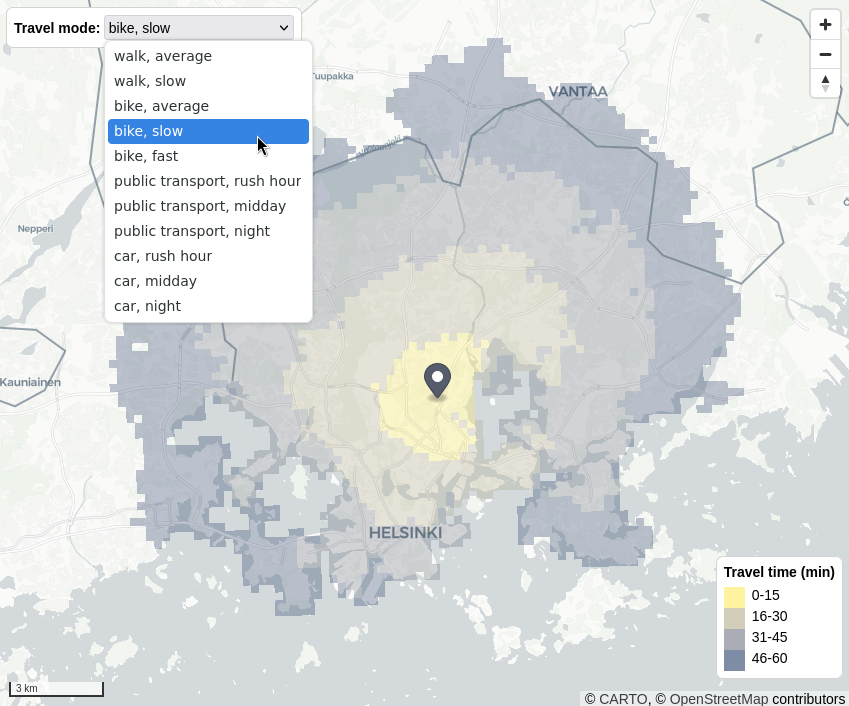
\includegraphics[width=0.9\textwidth]{visual/figures/screenshots/digital_interactive_map.png}
	\caption{
		A screenshot of a digital interactive map about travel times.
		In digital interactive maps
		cartographic interaction happens through a graphical UI,
		where the map can be manipulated by the user.
		Here the user can, for example,
		change the extent of the map by panning and zooming,
		and change the mapped data by selecting different options in a drop-down menu.
	}
	\label{fig:digital interactive map}
\end{figure}

\begin{figure}[H]
	\centering
	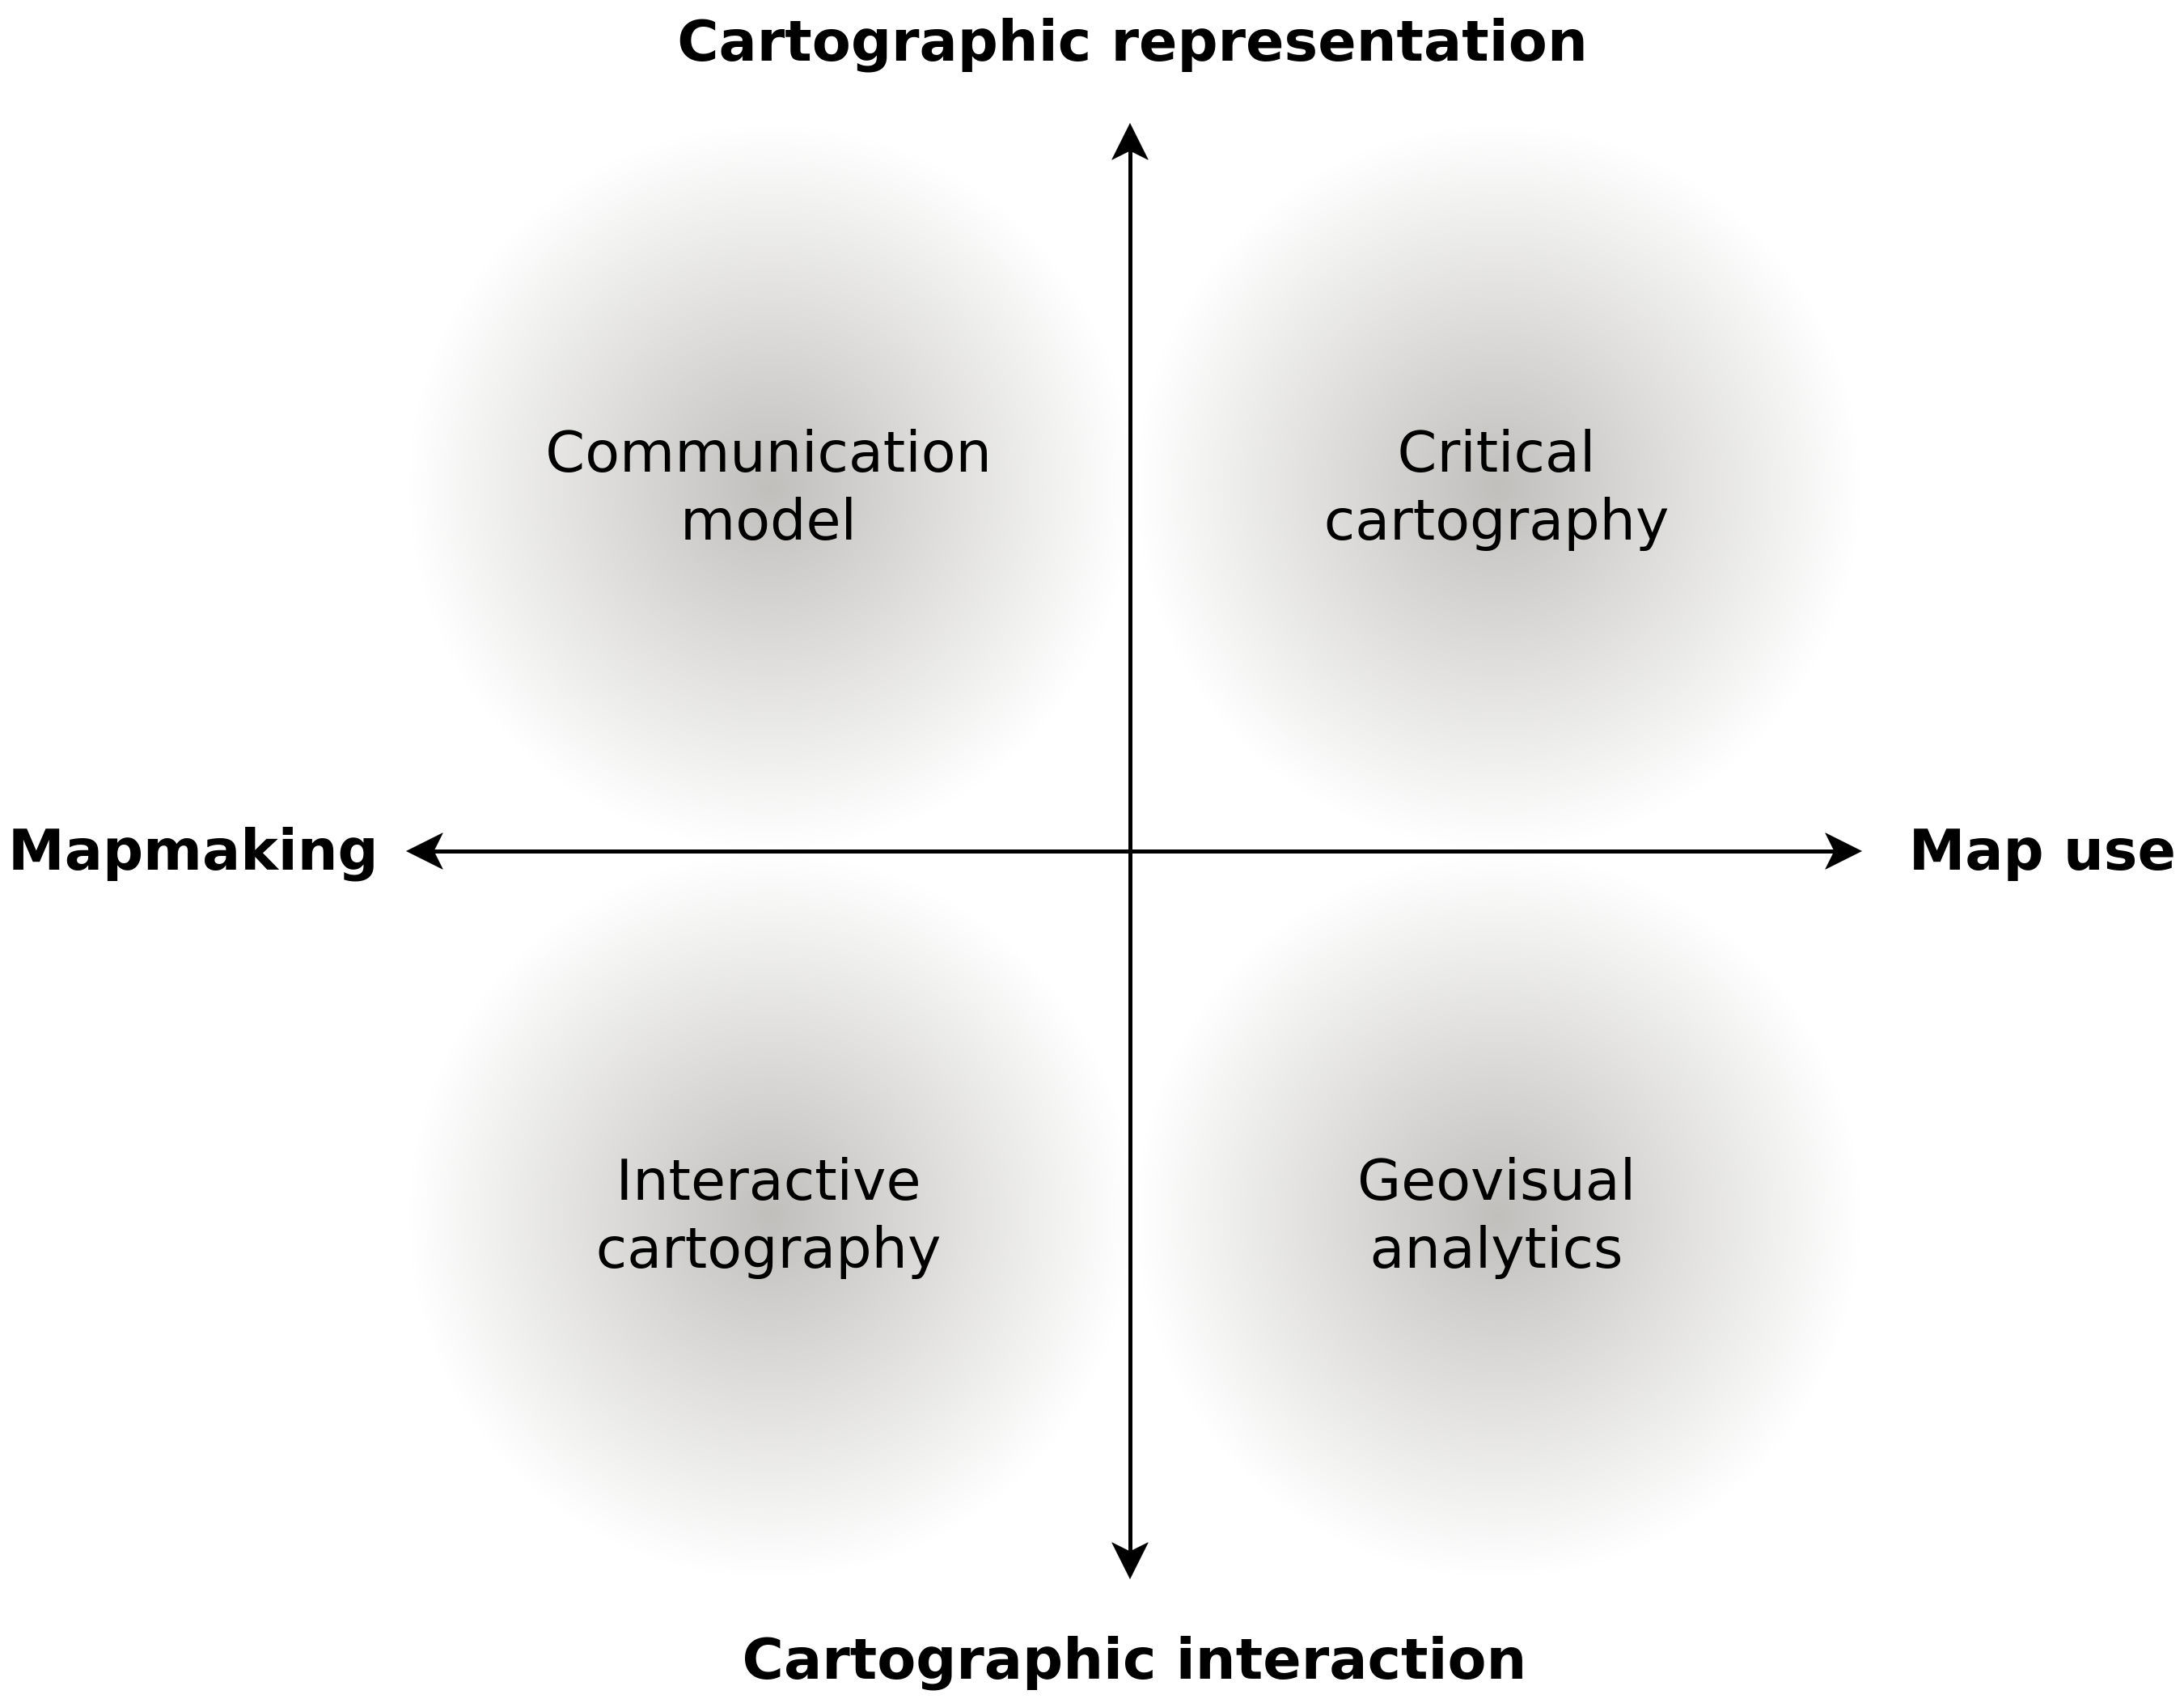
\includegraphics[width=\diagramwidth]{visual/figures/diagrams/cartography_topics.png}
	\caption{
		Interactive cartography as a topic of research
		in relation to other notable topics within cartography.
		The circles representing topics are fuzzy to imply that,
		instead of clear separation,
		different topics and areas of research blend into each other.
		Adapted from \textcite{rot2013b}.
	}
	\label{fig:cartography topics}
\end{figure}


In this thesis I approach cartographic interaction as
two-way communication between a map and a map user,
but limit it to digital maps and \acrshort{hci}.
As defined by \textcite[p.~14]{rot2011},
\enquote{\textit{cartographic interaction is the dialogue between a human and a map
mediated through a computing device}}.
The dialogue, or two-way communication, is a crucial aspect of this definition
as it makes explicit that in addition to the map user manipulating the map,
the map also affects the user:
The map user's interactions result in changes in the map,
and those changes, through the map user perceiving, interpreting and evaluating them,
can alter the map users goals and intentions
in further manipulating the map (figure \ref{fig:map interaction}) \parencite{rot2012}.
This conceptualization of cartographic interaction
is based on \posesscite{nor1988}
stages of action model that,
in contrast to many other theories on human-object-interaction,
places agency to both the human and the object.
Another aspect worth noting in \posesscite{rot2011} definition
is the notion of interactive maps as digital applications.
This is a relevant approach considering
that the mediums in which people interact with maps today
are predominantly and increasingly digital \parencite{mei2019}.
Digital environments also enable more ways to interact with maps
and to construct interactive map presentations \parencite{rot2013b, mei2019}.
Considering the aforementioned definition of cartographic interaction,
I deduce that, in the context of this study,
an \textit{interactive map} is a digital one,
and for it to be considered interactive it has to
facilitate a dialogue by enabling and adapting to manipulation by the map user.

\begin{figure}[H]
	\centering
	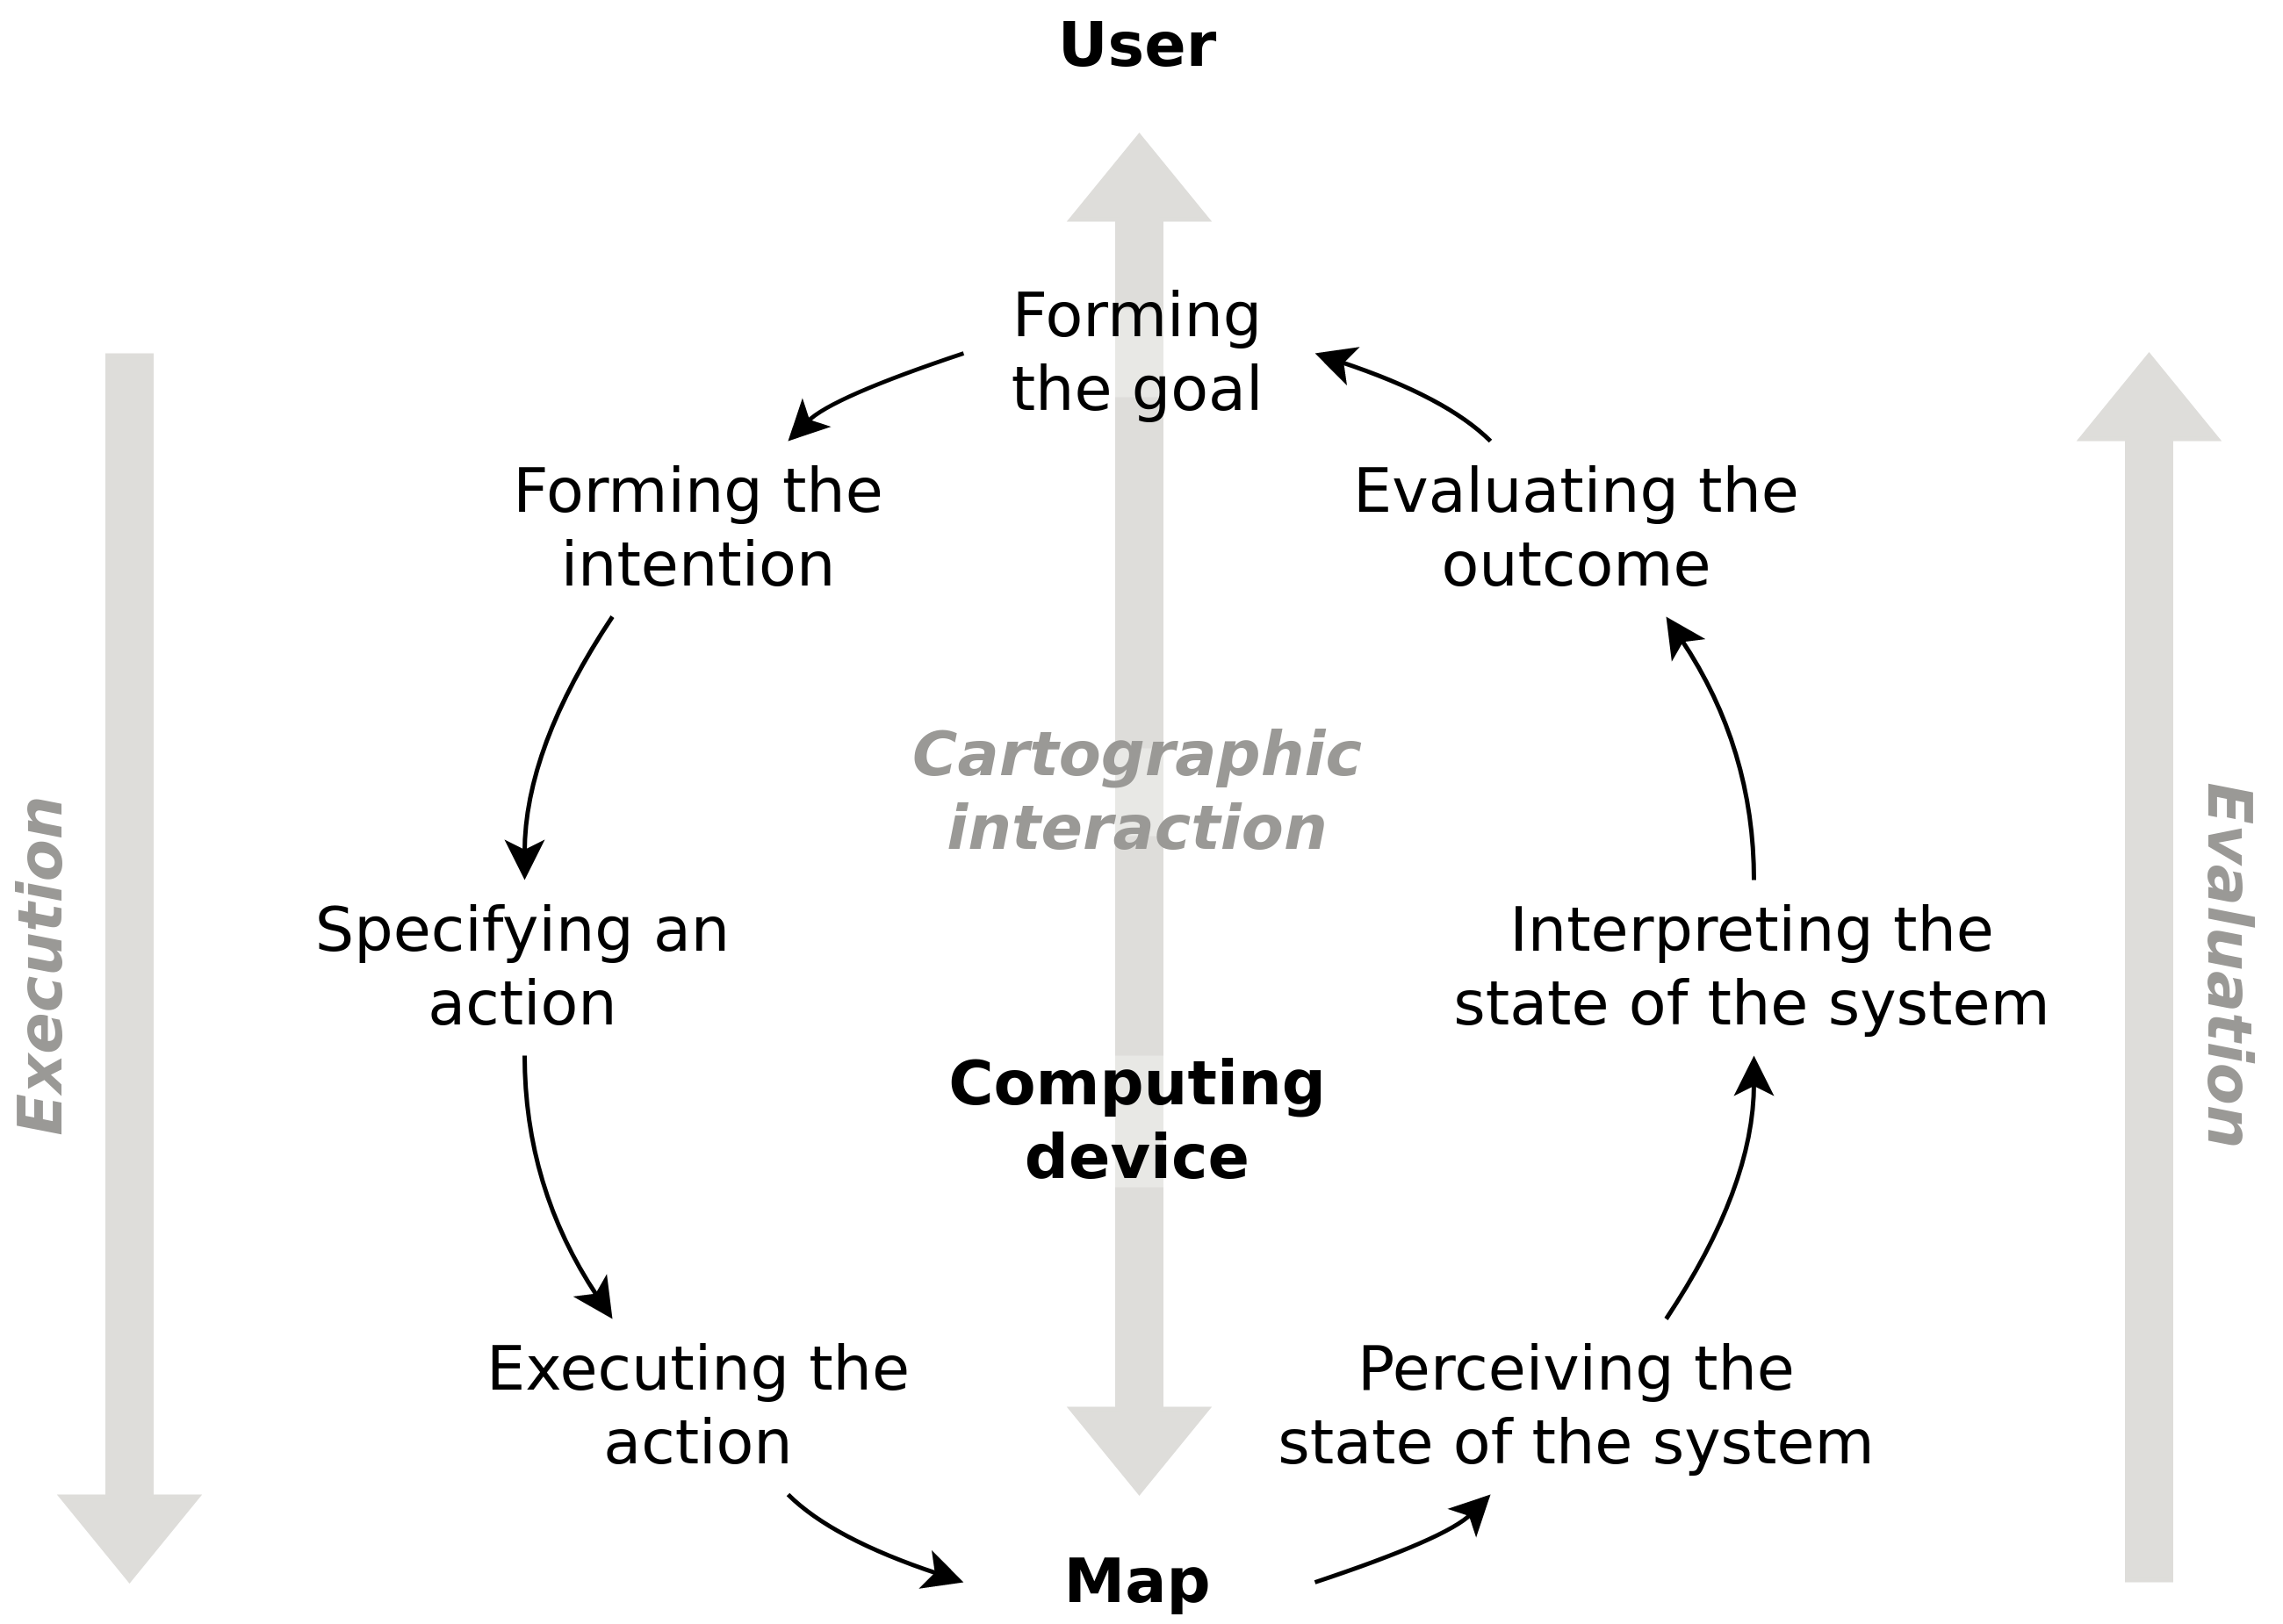
\includegraphics[width=\diagramwidth]{visual/figures/diagrams/map_interaction.png}
	\caption{
		The process of cartographic interaction.
		\posesscite{nor1988} stages of action model,
		a foundation of the concept of human-object-interaction as dialogue,
		is here applied to cartographic interaction.
		Adapted from \textcite{rot2012}.
	}
	\label{fig:map interaction}
\end{figure}


\subsubsection{Perspectives and disciplines relevant to interactive cartography}

Cartographic interaction, as defined above, has three components:
the human as the user, the map as the interface,
and the computing device as the technology that enables the interaction.
% Arguably, there is a fourth component too: the dialogue.  % TODO
While cartographic interaction as a concept should be approached as
the sum of its parts \parencite{rot2013b},
studies on cartographic interaction can take on perspectives
that emphasize given subsets of these components.
For example, \textcite{col2009} approach the topic from a user-centric perspective,
\textcite{rot2013a} has an interface-centric focus in
taxonomizing various interaction primitives in map interfaces,
and \textcite{oym2021} develop a technological method and an implementation
for producing interactive maps.
I should also stress that I do not wish to imply that these studies
only recognize the singular components of cartographic interaction
I've associated with them here.
Rather, they approach the topic from a perspective relevant to their respective goals,
but they do account for the other components as well.

% HCI
The components of cartographic interaction widen the scope of cartography,
also further motivating and calling for
multidisciplinary approaches in the field \parencite{rot2013b}.
As maps become interfaces,
\acrshort{ui} and \acrshort{ux} research and design becomes
part of the process of mapmaking \parencite{rot2015}.
Thus, the research, theories and methods in \acrshort{hci}
and usability engineering (\acrshort{ue}) have been notable influences
digital interactivity has introduced to the discipline of cartography \parencite{rot2017}.
These can for example be new empirical approaches such as
data acquisition through system or application level recording and storage of
user interactions with digital map interfaces \parencite{oom2015}.
Research on the different technological aspects and modes of \acrshort{hci}
has also been carried out in cartographic contexts,
for example by evaluating different input devices and methods
used in interacting with web map applications \parencite{wu2011}.

% UE
The usability of interactive map presentations has been studied with
usability metrics often employed in \acrshort{ue} research more widely.
These include but are not limited to
user satisfaction (how content users are with an interface having used it),
efficiency (how quickly users complete tasks with an interface)
and effectiveness (how successful users are at completing tasks with an interface)
\parencite{col2009}.
When considering usability, it should also be noted that interactive maps,
often relying solely on computer graphics for all aspects of their interface,
can introduce notable usability issues
to people without the capabilities to interact with such interfaces \parencite{duc2018}.
These issues can stem from the more general limitations of accessing digital applications --
for example lack of technical knowledge or unfamiliarity with a specific interface \parencite{kul2019} --
but are especially severe when it comes to visual impairments,
potentially leading to complete exclusion from accessing an interface \parencite{duc2018}.
Still, it has been shown that cartographic interaction can be made inclusive:
By introducing methods such as tactile and audio interaction,
interactive maps have been observed to be more efficient and satisfactory interfaces
for visually impaired users when compared to tactile static maps \parencite{bro2015}.
In general, as informed by \acrshort{ue},
the need for user perspective in studies on cartographic interaction has been recognized,
and user-centred and inclusive design practices are considered beneficial to map interface design
\parencite{niv2007, rot2017, duc2018}.

Even though briefly mentioned earlier,
geovisual analytics should also be highlighted as
a discipline that is especially relevant to interactive cartography.
Defined as \enquote{the science of analytical reasoning with
spatial information as facilitated by interactive visual interfaces}
\parencite{rob2017b},
it is clear that the field is largely enabled by
cartographic interaction.
In contrast to research in \acrshort{hci} and \acrshort{ue} --
both fields that are focused mainly on interfaces as primary objects of study
\parencite{mol2023, car1997} --
studies in geovisual analytics are more concerned with
how map interfaces enable and support analytical processes \parencite{rob2017b, and2010}.
An analytical process in this context consists of, for example,
assessing data and extracting insight from it (exploration),
studying and contrasting different insights (analysis),
disseminating results (presentation),
and integrating and reasoning about different insights and results (synthesis) \parencite{mac2017, dib1990}.
From the perspective of cartography and especially cartographic interaction,
this type of approach relates the map interface to many different stages and types of reasoning.
Thus, an interactive map can, often simultaneously, be
an interface to a multitude of analytical methods,
an analytical method in and of itself,
a means to satisfy many different analytical goals and needs,
and a platform for various methods and modes of interaction \parencite{rot2013b, rot2015}.

In the cartographic context,
the role of interactivity has often been considered most essential to
exploration and analysis \parencite{eds2008}.
At these stages of the analytical process,
the creation of numerous and / or highly interactive maps
enables rapidly gaining and assessing insights,
while the stages of synthesis and presentation
have classically been seen to employ fewer,
more static, presentations
(figure \ref{fig:analytical process interaction}) \parencite{dib1990}.
While interactive maps are still often connected to exploration,
their potential in presenting known insights (for example \textcite{ecc2008}),
as opposed to only revealing new ones through exploration,
has been recognized and growingly applied \parencite{fis2021}.
This proliferation of cartographic interaction is also visible in the state of mapmaking:
in practice, interactivity is being increasingly utilized
in most contexts where maps are present \parencite{fis2021, mei2019, rot2015}.

\begin{figure}[H]
	\centering
	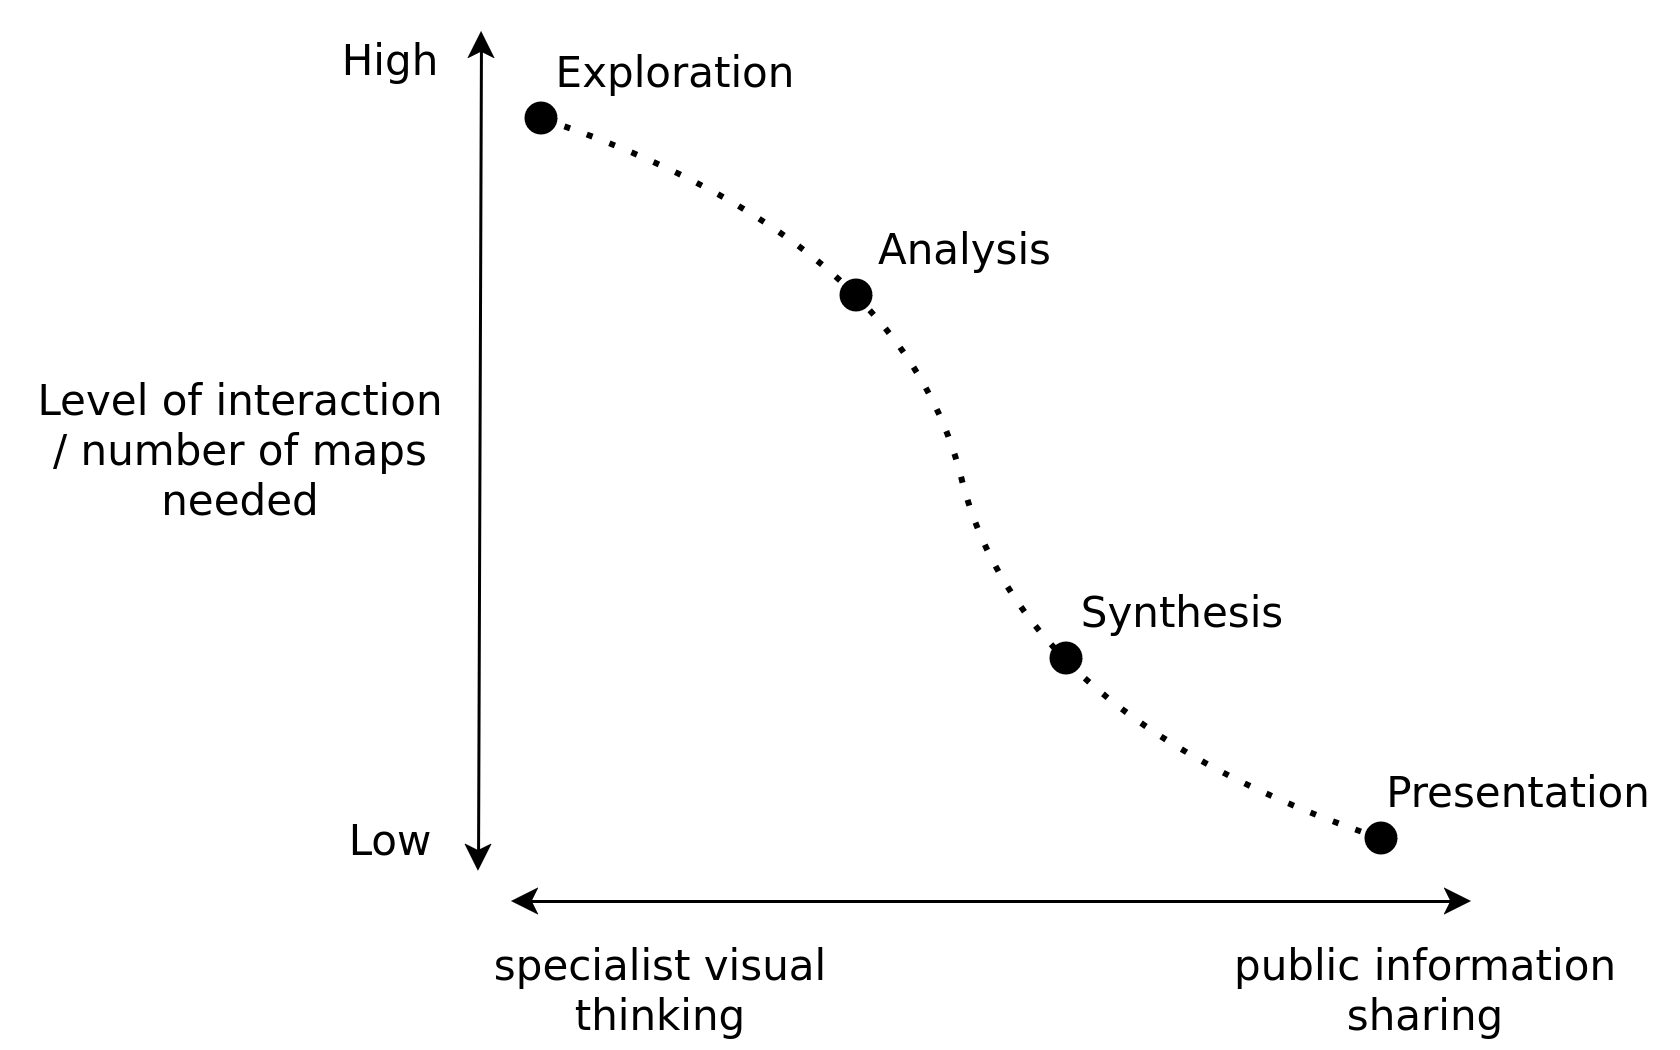
\includegraphics[width=\diagramwidth]{visual/figures/diagrams/swoopy.png}
	\caption{
		The need for interactivity at various stages of an analytical process.
		Considering the developments in cartography since 1990,
		the slope might be slightly gentler today.
		Adapted from \textcite{dib1990} with minor changes in wording based on
		\textcite{rot2015, mac1997}.
	}
	\label{fig:analytical process interaction}
\end{figure}


\subsubsection{Deconstructing the map interface}

What exactly an interactive map is,
or what kind of interaction exchanges a user can carry out with the map,
varies greatly.  % depending on what the purpose of the map is.
As is clear based on the above,
the applications of cartographic interaction are immensely diverse,
and so are the different types of map interfaces.
Thus, conceptualizing the many forms of
interactive maps and the interactions they enable
at a detailed level is no simple task.
Soon to be 20 years ago,
\textcite{tho2005} considered the comprehensive
identification, characterization and compilation
of the various types of interactions in visual analytics a
"grand challenge of interaction":
a prerequisite for the effective design and utilization of
interactivity in analytical processes.
Since then, and also predating \posesscite{tho2005} work,
this research topic has been widely explored in many relevant fields.
In an extensive literature review \textcite{rot2012}
provides a synthesis of tens of studies
that propose varying taxonomies of interaction,
especially in the context of interactive maps.
As a high-level output of the study, \citeauthor{rot2012}
classifies interaction taxonomies into three categories:
Objective-based, operator-based and operand-based.
Objective-based taxonomies categorize interactions based on
the objective behind the interaction,
for example to select, explore or encode \parencite{yi2007},
while operator-based taxonomies act at the level of operations such as
zooming, panning or altering representation types \parencite{eds2008}.
Operand-based taxonomies classify interactions based on what is operated upon.
This could be, for example, data, the representation of said data,
or the interface itself \parencite{cra2002}.

Building upon these insights,
\textcite{rot2013a} proposed a taxonomy of interaction in a follow-up study.
While, again, multiple such efforts exist,
\citeauthor{rot2013a}'s taxonomy is perhaps the most relevant in this case:
It is constructed from the perspective of cartographic interaction,
and informed not only by a review of other taxonomies \parencite{rot2012}
but also by empiric studies with experts in the field of interactive cartography
\parencite{rot2013a}.
This taxonomy is based on \textit{interaction primitives} --
basic units of interaction that, when combined,
make up complete interaction exchanges between a map and a map user.
These interaction primitives are grouped into 4 dimensions:
\textit{objectives}, \textit{operators} and \textit{operands} as already described above,
with the addition of user \textit{goals} as a broader context of
an interaction exchange \parencite{rot2013a}.
As another added level of detail, operator primitives are split into primitives that
enable work and primitives that represent the work itself,
and operand primitives are split into targets that are operated
upon and levels on which the operation happens.
\enquote{Level} in this context means the scope of the operation:
either elementary (one element) or general (multiple elements) \parencite{rot2013a}.
For the complete taxonomy, see table \ref{tab:interaction primitives}.

\begin{table}[H]
	\caption{
		\posesscite{rot2013a} taxonomy of interaction primitives.
		A taxonomy such as this is required for the systematic description, study and design
		of map interfaces.
	}
	\label{tab:interaction primitives}
	\centering
	\begin{tabular}{ | L{0.15\textwidth} | L{0.75\textwidth} | }
		\hline
		\textbf{Dimension}
		& \textbf{Primitives} \\
		\hline
		\hline
		Goals
		& Procure, predict, prescribe \\
		\hline
		Objectives
		& Identify, compare, rank, associate, delineate \\
		\hline
		Operators
		& \tabitem Enabling operators: import, export, save, edit, annotate \\
		& \tabitem Work operators: reexpress, arrange, sequence, resymbolize,
		overlay, reproject, pan, zoom, filter, search, retrieve, calculate \\
		\hline
		Operands
		& \tabitem Target operands: space-alone, attributes-in-space, space-in-time \\
		& \tabitem Level operands: elementary, general \\
		\hline
	\end{tabular}
\end{table}


In general, interaction primitives
address the \textit{what} in an interaction exchange:
for example, what the goal is, what the operation is, or what is operated upon.
A wider theoretical framework of interaction, such as the one presented in
section \ref{defining cartographic interaction and interactive map},
is necessary to understanding \textit{how} interaction works as a whole.
What I have not yet covered in detail is
\textit{how} interactions are carried out at the level of the interface, or,
in other words, how the interactivity is provided to the user.
In the context of \acrshort{hci},
the ways in which a user can interact with a system are referred to as
\textit{interaction styles} \parencite{shn1995}
(sometimes also \textit{interface styles} \parencite{how1996}).
These are conventionally categorized into 4 main styles:
\textit{command language},
\textit{form fill-in},
\textit{menu selection} and
\textit{direct manipulation}
\parencite{soe2015}.
Additions exist, for example \textit{natural language},
often employed in audio-based interfaces \parencite{duc2018}.
Most of the aforementioned interaction styles are quite self-explanatory,
but one; direct manipulation, depends on context.
In the case of cartographic interaction,
it refers most often to direct interactions with the map \parencite{rot2012}.
A common example would be a case where the \textit{pan} operator primitive
is executed by dragging the map with a pointing device.

When considering a map interface,
it should be noted that most operator primitives
can be exposed to the user using multiple interaction styles.
For example, the previously mentioned \textit{pan} operator could just as well
be executed with a command language, a form fill-in, or a menu selection.
What interaction style is best suited for a given operator is a question
of \acrshort{ui} and \acrshort{ux} design,
and depends heavily on the specific operator as well as
the users and the use case of the map interface \parencite{rot2015}.
This further exemplifies the diversity of interactive maps,
as interaction style adds yet another dimension to conceptualizing the
function and form of a map interface.
When assessing the interaction styles in a map interface,
one aspect that is often considered in interactive cartography
is the amount of direct map manipulation in relation to other interaction styles.
If direct map manipulation is just part of
the interaction styles provided by an interface,
the interface might be called
a \textit{map-based system} or a \textit{map-based interface}
instead of, for example,
an \textit{interactive map} or a \textit{map-interface} \parencite{rot2013b}.
A desktop \acrshort{gis} software could represent the former type of interface (figure \ref{fig:qgis}),
and a simple web map the latter (figure \ref{fig:simple web map}).

\begin{figure}[H]
	\centering
	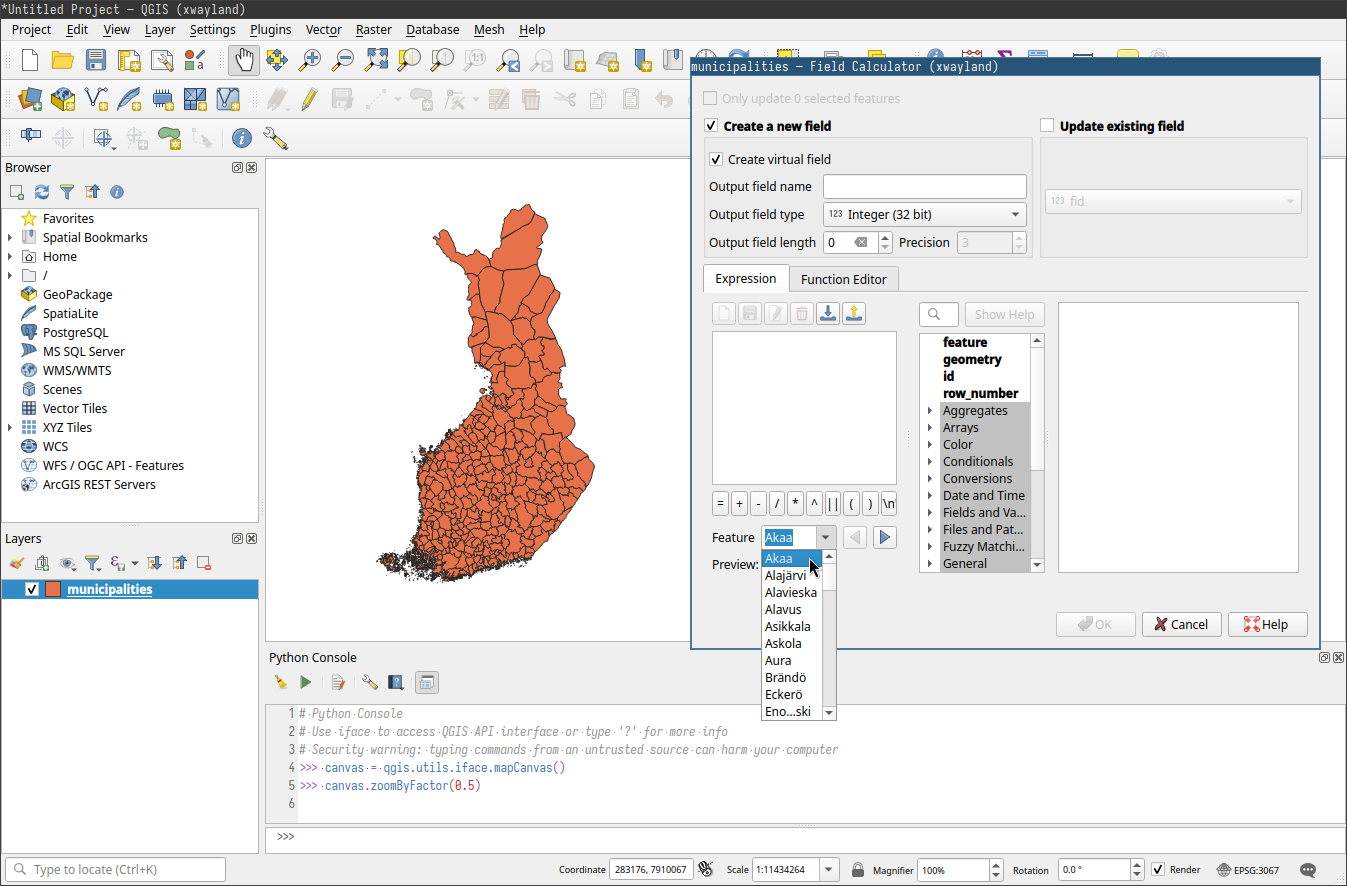
\includegraphics[width=0.9\textwidth]{visual/figures/screenshots/qgis_interface.png}
	\caption{
		The UI of the desktop GIS QGIS \parencite{qgis}.
		GIS software often supports a wide array of interaction primitives and,
		consequently, interaction styles:
		Direct manipulation, menu selection, form-fill in and command language
		can all be seen in this image.
	}
	\label{fig:qgis}
\end{figure}

\begin{figure}[H]
	\centering
	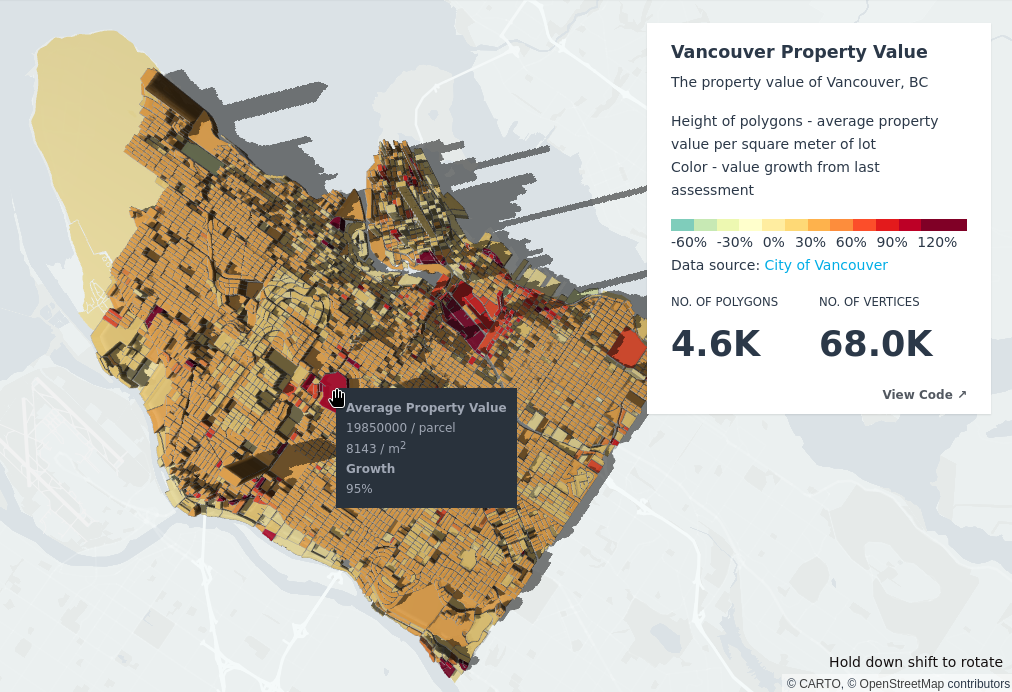
\includegraphics[width=0.9\textwidth]{visual/figures/screenshots/simple_web_map.png}
	\caption{
		An interactive web map with a single interaction style:
		direct manipulation of the map.
		Map source: \textcite{deckgl-ex}
	}
	\label{fig:simple web map}
\end{figure}

% Together with interface types the interaction primitives make up
% the building blocks necessary for understanding, analysing and designing map interfaces.


% cra2002
% Interaction with data representation (zoom, pan, symbolization)
% Interaction with the temporal dimension (animations, toggling, sorting)
% Interaction with data (exploration)
% Interaction to contextualize (multiple views, overlay)

% hee2012
% Data & view specification (visual encodings, filtering, sort)
% View manipulation (select, navigate, organize views and workspaces)
% Interacting with processes & preserving analytical provenance (record and review actions (meta-interaction))

% yi2007 (intent-based)
% 1) Select, 2) Explore, 3) Reconfigure, 4) Encode, 5) Abstract/Elaborate, 6) Filter, and 7) Connect

% rot2012 the framework

% rot2013a
% Goals: procure, predict, & prescribe
% Objectives: identify, compare, rank, associate, & delineate
% (increasing in sophistication);
% Operators: import, export, save, edit, & annotate (enabling);
% reexpress, arrange, sequence, resymbolize, overlay, reproject, pan, zoom, filter, search, retrieve, & calculate (work);
% Operands: space-alone, attributes-in-space, & space-in-time (search target);
% elementary & general (search level)



% Interactive
% In the following, the term “in-teractive” is used rather than “dynamic” to distinguish display updates evoked by the user(interaction) from display updates evoked by the system (such as animation, a form of car-tographic representation)phy - broadly  % FIXME copypasta


% \parencite{kra2017}
% The traditional ‘authoritative’ view of the map being a carefully crafted product
% by the cartographer, aimed at visually communicating a complete, mostly static database
% of known geographic facts to a user, has turned into a participatory and collaborative perspective.
% The map has moved beyond the static window to the world and become an
% interactive, mobile, dynamic and collaborative interface between a human, groups of
% people and the dynamically evolving environment



% The nature of interactive cartography
% More than a map: ui, ux
% What even is an interactive cartographer?
% A map is both the for of presentation, as well as the method of interaction
% -> a more complex map means basically a user interface -> need for UI library
% \textcite{rot2013a, rot2013b}

\subsection{Crafting interactive maps}
\subsubsection{Maps as digital applications}

Technological implications of map interaction,
technology being an enabling and a limiting factor in map interaction.

% The influence of technology on interactive maps and cartography.
% Also, the mapmaker is more often a software developer than a cartographer.
% How much of innovation is more of "this is cool",
% versus "this is a cartographically informed way to present something".

The platforms on which interactive maps are used:
Desktop software, mobile, web ...

Previous section provided the tools to conceptualize what an interactive map is,
this section aims to add the necessary insight to implement map interfaces in practice.

\subsubsection{Web mapping technologies}

% rot2014
Why web-based applications are the norm
(in general and, for much of the same reasons, in the context of maps).

Define web map

The relevant terms and software architechture (in web context):
At least the concepts of front / backend and server requests / responses
are pretty essential to understanding anything about the technical side.

The relevant technologies, the tools with which interactive maps are made:
web mapping and user interface libraries, backend solutions
(not every technology but a concise overview)

\subsection{Cartographic presentation of accessibility}

Different conceptualizations of accessibility,
their implications in presenting the phenomenon.

In general: people, transport, activities make up accessibility.
A multi-location, multimodal, multi-temporal phenomenon.

Approaches in visualizing accessibility:
Examples of static and interactive accessibility maps.
Simple measures vs complex measures,
High interactivity vs low interactivity.

Isochrones as an example of a simple measure / visualization approach:

\begin{figure}[H]
	\centering
	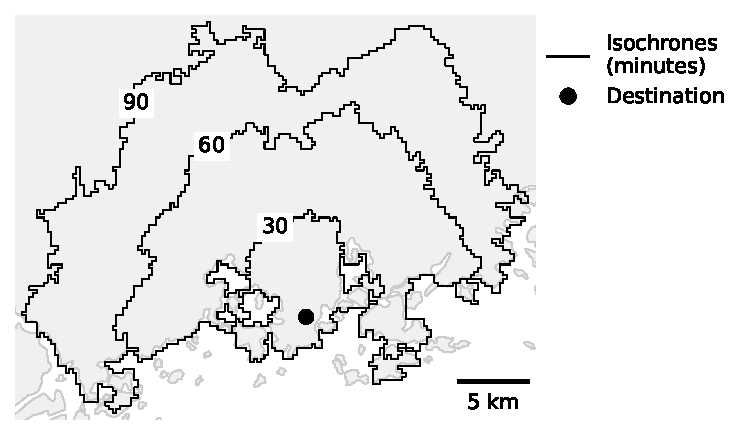
\includegraphics[width=0.6\textwidth]{visual/figures/ttm/isochrone_lines.pdf}
	\caption{Isochrones}
	\label{fig:isochrone lines}
\end{figure}

\begin{figure}[H]
	\centering
	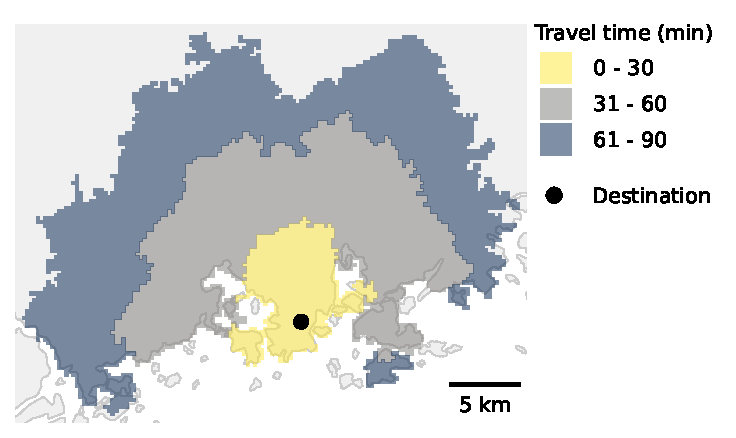
\includegraphics[width=0.6\textwidth]{visual/figures/ttm/isochrone_areas.pdf}
	\caption{Areas between isochrones}
	\label{fig:isochrone areas}
\end{figure}

SIDENOTE: How should I refer to isochrones when I mean the polygons instead of lines?

% TODO
% Mention tradeoffs (detail - speed) -> leads to methods
% Crafting any cartographic presentation is much about tradeoffs.
% Often these tradeoffs are concerned with the visual composition of the presentation --
% what the map can and should try to communicate.

% TODO
% Previous presentations can be very precise, but locked to a single place


% TODO add tech / software table?
\section{Materials and methods}

\subsection{Study design}

The study had two main goals.
Firstly, I aimed to develop a map interface for
interactively presenting an extensive spatial dataset on travel times,
and through the development process assess
the tools and options available for making such a map.
More precisely,
I focused on the choice of web mapping library
and on the different approaches in preprocessing the mapped data.
The goal was to find how,
and to what extent,
these factors affect the map interface.
The second goal was to understand how map users utilize such a map interface,
and how the interactive map works as a representation.
Here I employed a survey to find out how
people use the map when given different tasks to complete with it,
and whether a highly interactive presentation approach affects
how map users perceive the mapped phenomenon and interpret the map.
These two themes, the development process and the survey,
make up the two high-level components of the study.

% While the primary goal of the development process was
% to produce the map presentation and enable the survey,
% the development process in and of itself was crucial to the study as well.
% Its purpose was to be the framework that
% allows for answering the research questions
% about the more technology-centric aspects of
% the making of an interactive map.

Pragmatically speaking, a large part of this study was
a software development project to produce a functional web map application,
and the parts that were not, were still reliant on
the software development project succeeding.
This naturally affected the study design.
It allowed for freedom in crafting a map interface made exactly for this study,
but also introduced limitations
as any functionality to be included in the map, and in the study,
had to also be implemented.
In other words, the technical implementation as well as the survey
had to be designed around what is meaningful to study,
but also based on what is realistic to implement.
To minimize the risk and uncertainty inherent to such a setting,
I heavily utilized modern software development methodologies
\parencite{saq2020, bec2001, sha2017, kuh2017}
in planning the development process and the study as a whole.
Based on these,
I formatted the following points of focus
to guide the development process:
\begin{itemize}
	\item Plan minimally and adapt the plan constantly.
	\item Prioritize a working state of the entire application over details in single components.
	\item Adapt to technical constraints at the start, not at the end.
\end{itemize}

By adhering to these principles I could at an early stage see
whether the study was realistic, and,
especially considering the more technology-centric side of the study,
hone in on what research questions were actually meaningful.
Iteratively improving the application as a functional whole
allowed me to consider the map interface
from the perspective of the map user as early as possible,
better integrating the survey into the study.
This is important as the map presentation is simultaneously an output of the development process
and an input to the design of the survey.

For an overview of the study design see figure \ref{fig:study design}.
% This allowed me to improve the relevancy of my research. TODO Discussion?
% I say this not only in the context of gaining valuable results to my research questions --
% I want to emphasize that to even know what research questions to ask is impossible with a linear approach.

% While the development process and the survey were linked to each other,
% they each had their separate goals and outputs too.
% In addition to producing the map presentation,
% the development process had to enable testing and answering my research questions
% about the making of an interactive map.
% This placed increased
% The goal of the survey is to gain insight on
% how the interactive map works as a representation of the mapped phenomenon.
% With the survey I collect data on map usage,
% which I in turn analyse to answer my research questions related to the map usage.

\begin{figure}[H]
	\centering
	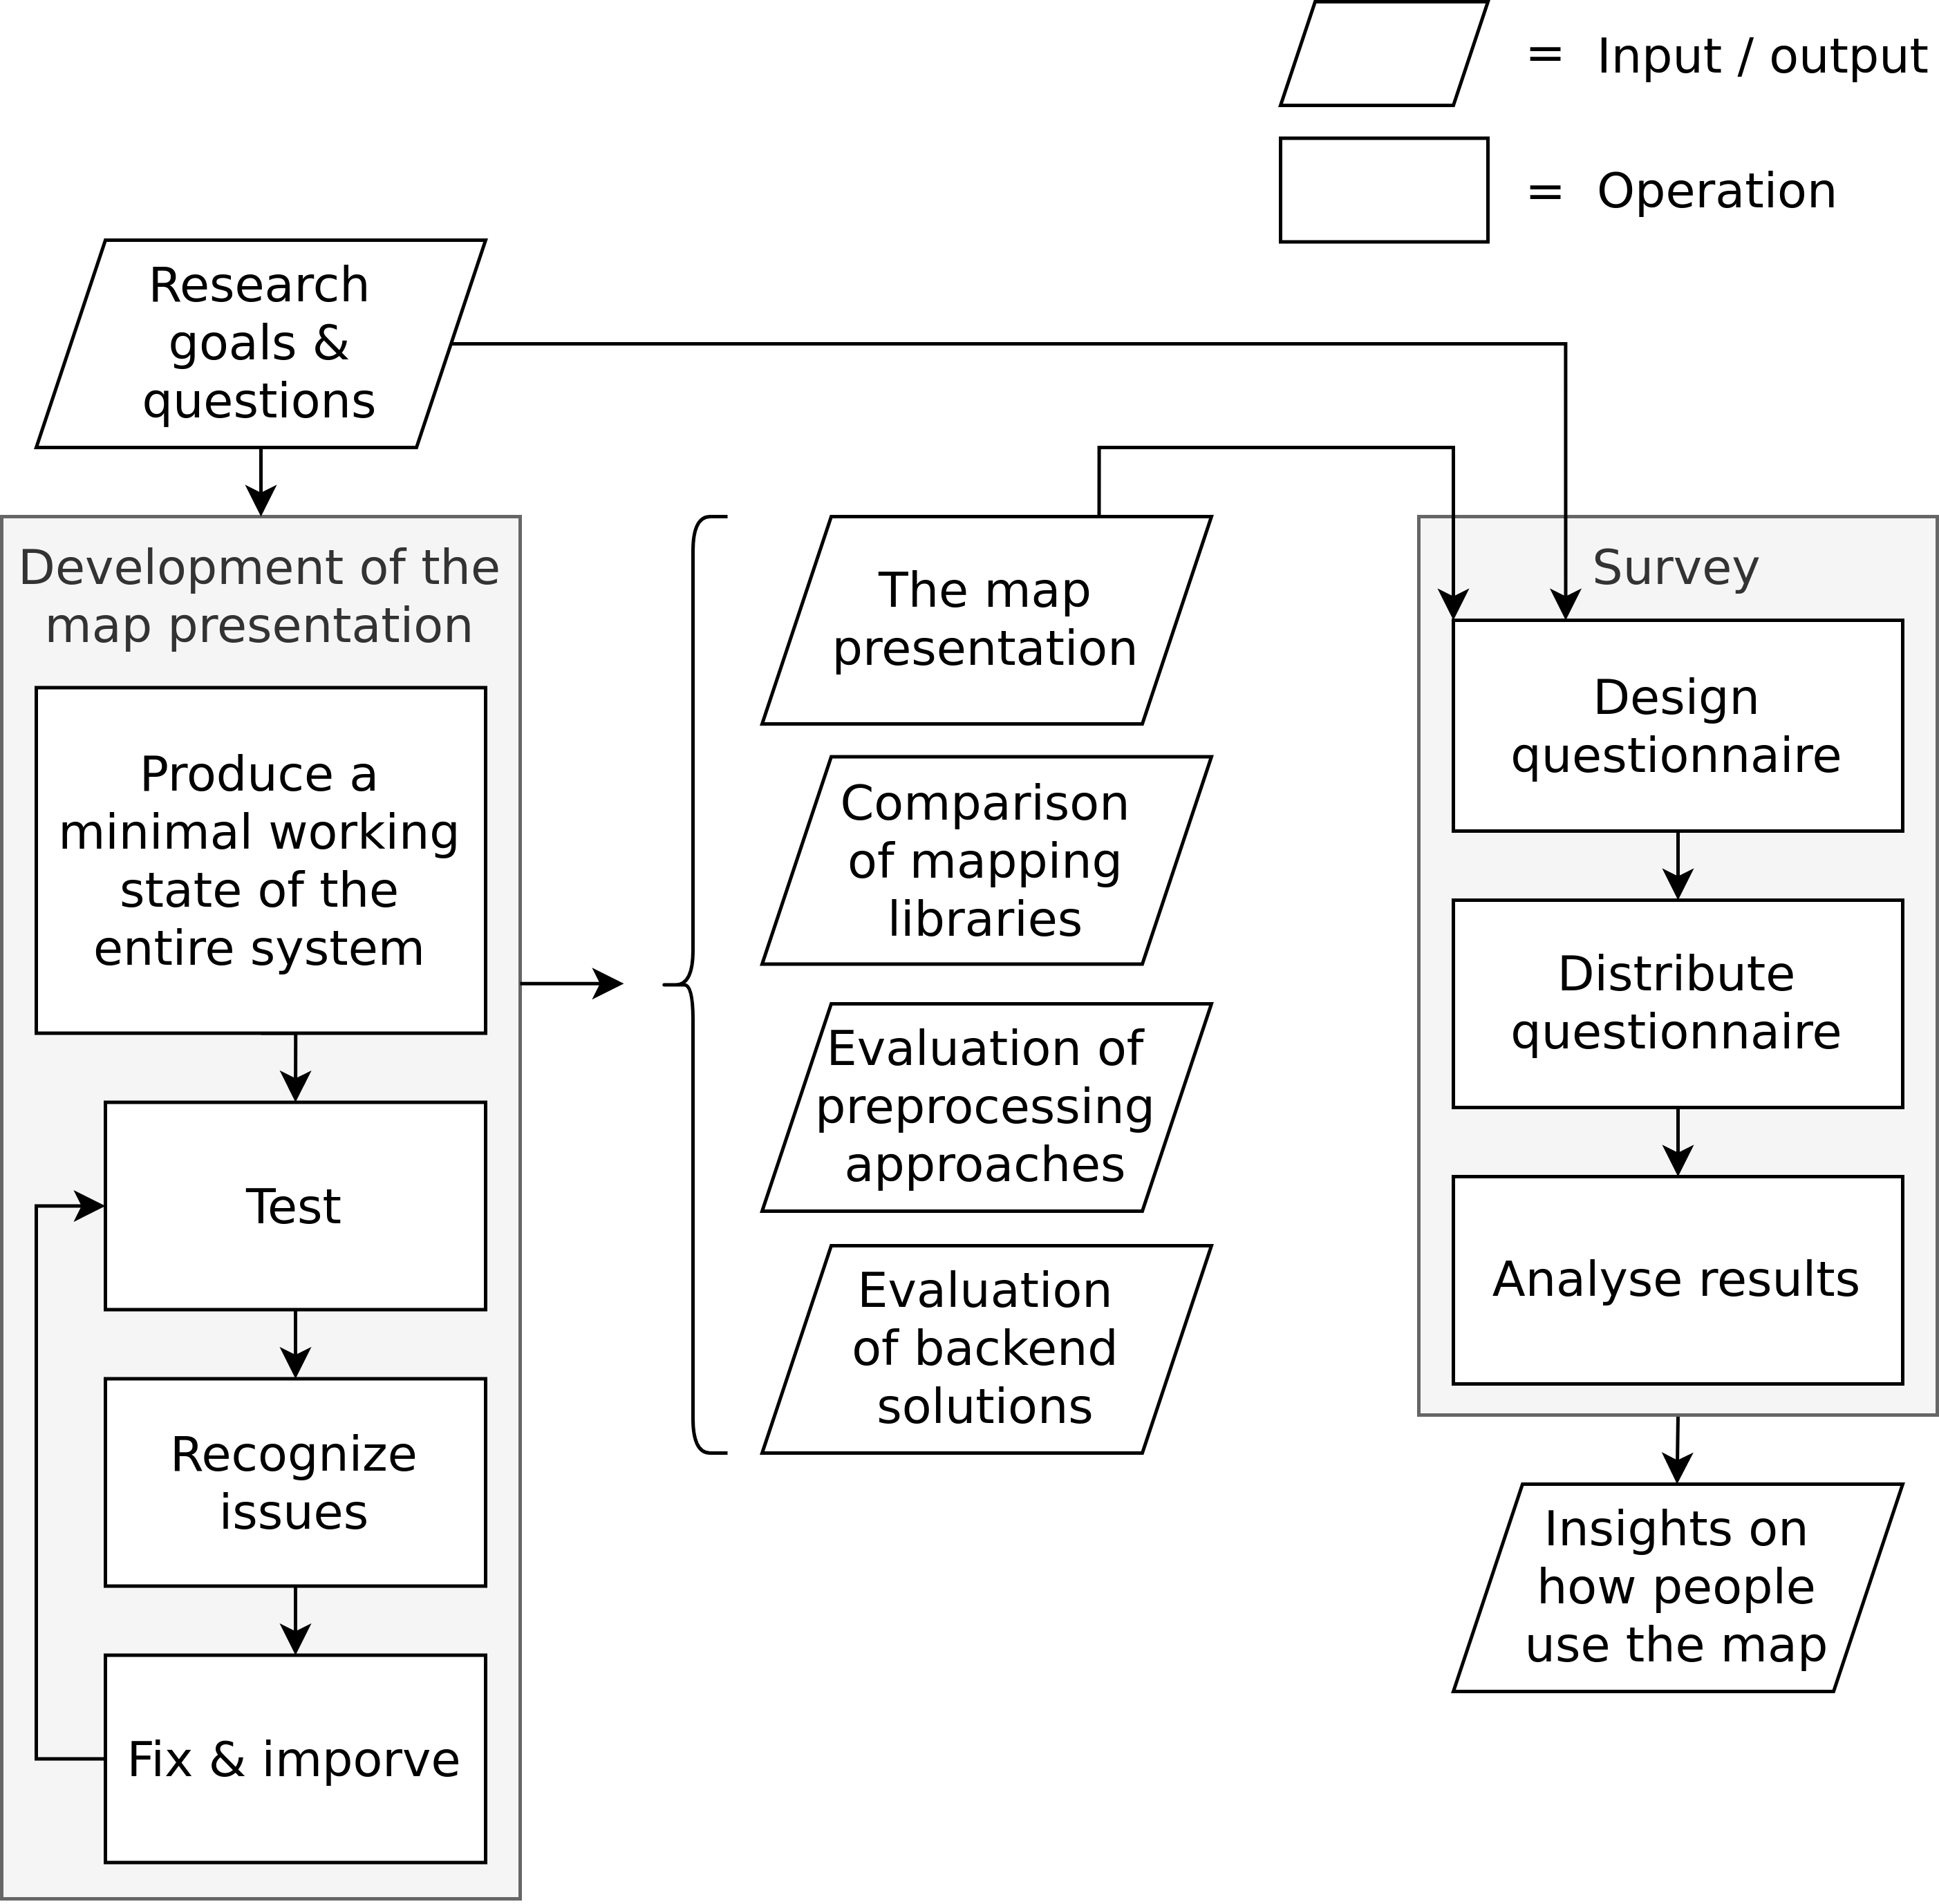
\includegraphics[width=\diagramwidth]{visual/figures/diagrams/study_design.png}
	\caption{An overview of the study design.}
	\label{fig:study design}
\end{figure}


\subsection{Data -- Helsinki region Travel Time Matrix}

The \acrlong{ttm} (\acrshort{ttm}) \parencite{fin2023}
is a dataset containing information of travel times and distances
in the Helsinki region in southern Finland.
This dataset was crucial to developing the map application,
as it was the sole source of the travel times shown on the map.
The dataset and the set of methods with which it is produced are open-source.

% Describe ttm in general: ykr, origin dest pairs etc (more surface level stuff common to all matrices)
A significant component of the \acrshort{ttm} is the \acrlong{ykr} (\acrshort{ykr})
statistical grid made by the Finnish Environmental Institute.
The grid has a spatial resolution of 250x250m, and it covers the entire Finland.
Most importantly, however, the part of the \acrshort{ykr} grid that overlaps with
the Helsinki region provides the spatial component for
the travel times stored in the \acrshort{ttm}.
The spatial extent of the dataset is shown in figure \ref{fig:ttm extent}.

\begin{figure}[H]
	\centering
	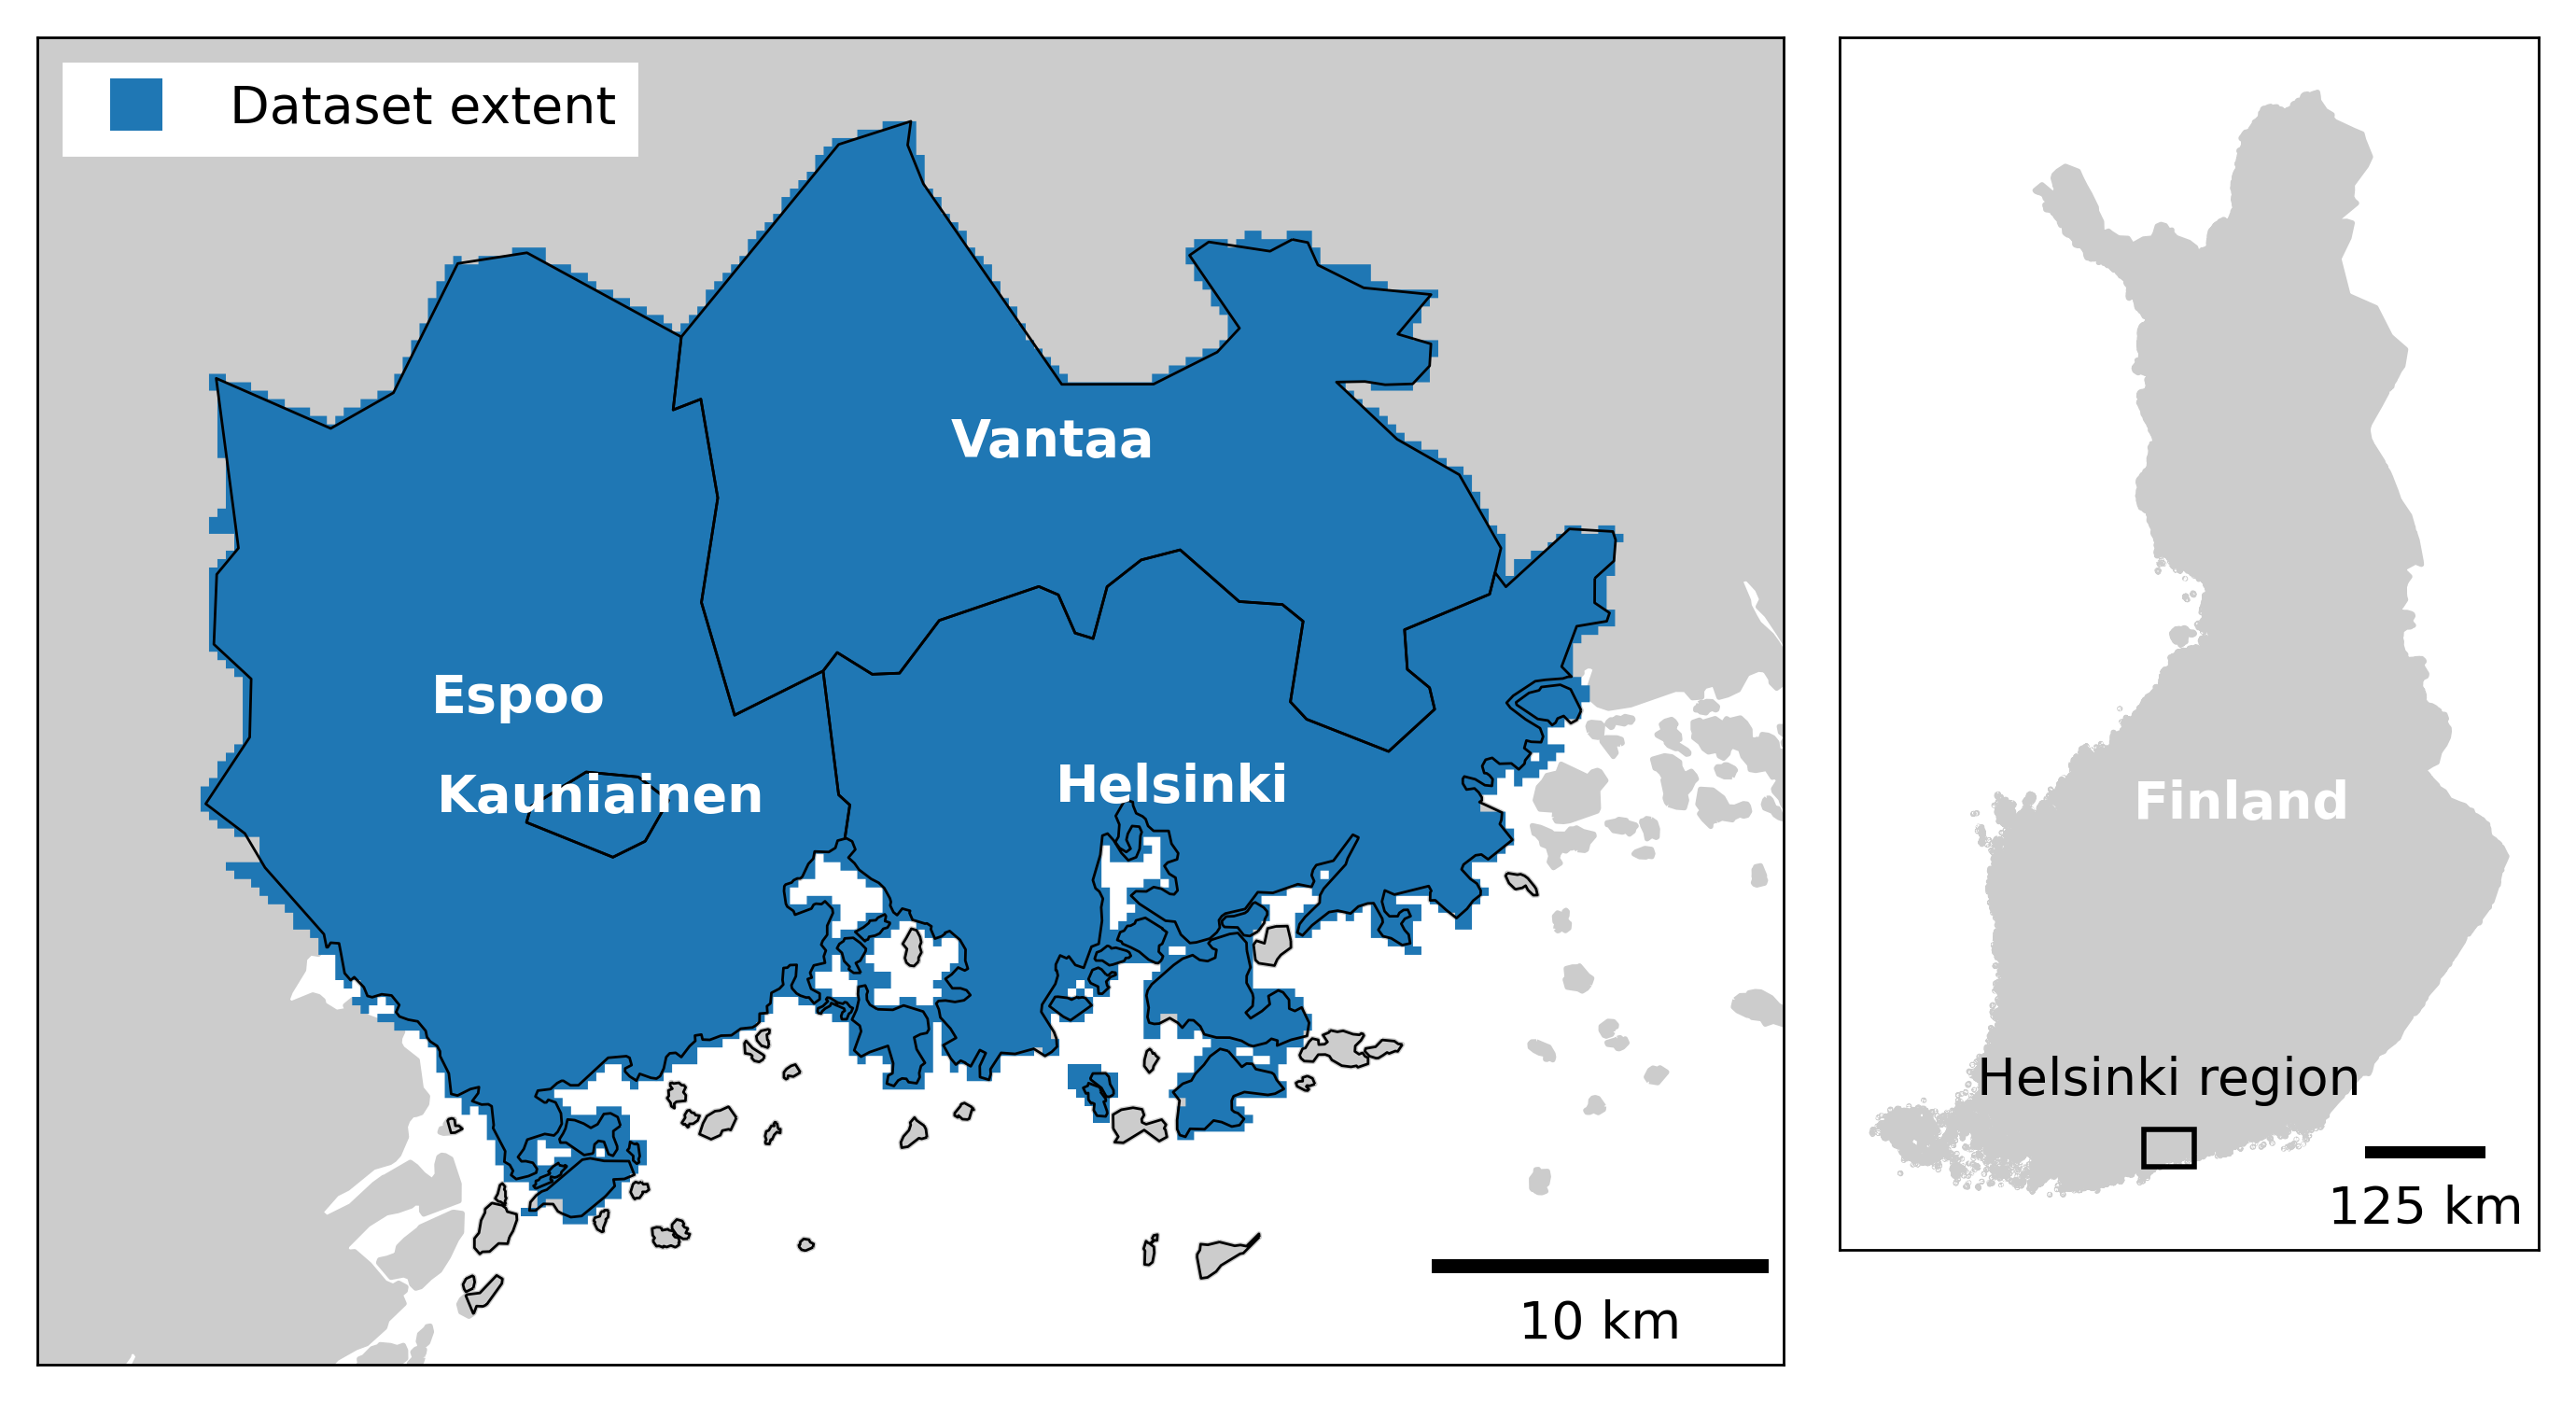
\includegraphics[width=0.9\textwidth]{visual/figures/ttm/ttm_extent}
	\caption{The location and extent of the TTM}
	\label{fig:ttm extent}
\end{figure}

The \acrshort{ttm} stores the travel times and distances
from every \acrshort{ykr} grid cell to every other  \acrshort{ykr} grid cell
within the Helsinki region.
The Helsinki region fits 13231 \acrshort{ykr} grid cells,
which means that the complete \acrshort{ttm} contains travel times and distances for
over 175 million routes.

All the routes are calculated for multiple different travel modes.
The primary travel modes are walking, cycling, public transportation and private car,
and, when applicable, each mode has variations based on
time of day and / or walking or cycling speed.
The time of day is especially relevant to motorized transport
in the form of the rush hour, for example,
while walking speed affects any travel mode
where a significant portion of the trip is covered on foot.
To be comparable with each other,
the travel times for all travel modes are
calculated with a \textit{door-to-door approach}
which accounts for things such as walking to a bus stop,
waiting for transfer times based on public transit schedules,
or locking and unlocking a bike \parencite{ten2020}.

% Describe the particular matrix (2023), methodology etc
\acrshort{ttm}s have been calculated for multiple years.
Differences between these datasets exist in the applied methodologies
and, thus, also in the content \parencite{ten2020}.
Also, the underlying city structure as well as the street and public transport networks
are by no means static over the years
which further introduces differences.
The map presentation I developed in this study
is based on the 2023 version of the \acrshort{ttm},
the newest one at the time of writing.
See table \ref{tab:ttm description} for an overview of the dataset,
and table \ref{tab:ttm table structure} for all the travel modes and
their variations included in the dataset.

\begin{table}[H]
	\caption{Descriptive values of the \acrshort{ttm}}
	\label{tab:ttm description}
	\centering
	\begin{tabular}{ | L{0.4\textwidth} | L{0.5\textwidth} | }
		\hline
		Spatial resolution
		& 250 x 250 m
		\\
		\hline
		Number of grid cells
		& 13231
		\\
		\hline
		Number of origin-destination pairs
		& 175 059 361
		\\
		\hline
		Travel modes
		& \tabitem walking \\
		& \tabitem cycling \\
		& \tabitem public transportation \\
		& \tabitem private car \\
		\hline
		Travel mode variations (if applicable)
		& \tabitem Time of day (rush hour, midday, night) \\
		& \tabitem Walking speed (average, slow) \\
		& \tabitem Cycling speed (average, fast, slow) \\
		\hline
	\end{tabular}
\end{table}


\begin{table}[H]
	\caption{The table structure of \acrshort{ttm} data}
	\label{tab:ttm table structure}
	\centering
	\begin{tabular}{ | L{0.15\textwidth} | L{0.75\textwidth} | }
		\hline
		\textbf{Column name}
		& \textbf{Description}
		\\
		\hline
		\hline
		from\_id
		& ID number of the origin grid cell
		\\
		\hline
		to\_id
		& ID number of the destination grid cell
		\\
		\hline
		walk\_avg
		& Travel time in minutes from origin to destination by walking at an average speed
		\\
		\hline
		walk\_slo
		& Travel time in minutes from origin to destination by walking slowly
		\\
		\hline
		bike\_avg
		& Travel time in minutes from origin to destination by cycling at an average speed; incl. extra time (1 min) to unlock and lock bicycle
		\\
		\hline
		bike\_fst
		& Travel time in minutes from origin to destination by cycling fast; incl. extra time (1 min) to unlock and lock bicycle
		\\
		\hline
		bike\_slo
		& Travel time in minutes from origin to destination by cycling slowly; incl. extra time (1 min) to unlock and lock bicycle
		\\
		\hline
		pt\_r\_avg
		& Travel time in minutes from origin to destination by public transportation in rush hour traffic, walking at an average speed
		\\
		\hline
		pt\_r\_slo
		& Travel time in minutes from origin to destination by public transportation in rush hour traffic, walking at a slower speed
		\\
		\hline
		pt\_m\_avg
		& Travel time in minutes from origin to destination by public transportation in midday traffic, walking at an average speed
		\\
		\hline
		pt\_m\_slo
		& Travel time in minutes from origin to destination by public transportation in midday traffic, walking at a slower speed
		\\
		\hline
		pt\_n\_avg
		& Travel time in minutes from origin to destination by public transportation in nighttime traffic, walking at an average speed
		\\
		\hline
		pt\_n\_slo
		& Travel time in minutes from origin to destination by public transportation in nighttime traffic, walking at a lower speed
		\\
		\hline
		car\_r
		& Travel time in minutes from origin to destination by private car in rush hour traffic
		\\
		\hline
		car\_m
		& Travel time in minutes from origin to destination by private car in midday traffic
		\\
		\hline
		car\_n
		& Travel time in minutes from origin to destination by private car in nighttime traffic
		\\
		\hline
		walk\_d
		& Distance from origin to destination, in metres, on foot
		\\
		\hline
	\end{tabular}
\end{table}




\subsection{Implementation of the map presentation}

\subsubsection{Software requirements}
\label{software requirements}

Software requirements are the functionalities and properties
that a given system should have,
as well as the constraints it must adhere to \parencite{chu2009}.
They are an essential aspect to consider in software development
as they are a way to explicate
what is being developed and what exactly is the framework
in which an implementation process is carried out \parencite{saq2020}.
Software requirements are often divided into
functional and nonfunctional requirements.
Functional requirements define the user-facing features of the system
while nonfunctional requirements describe the properties of a system
\parencite{chu2009}.
Nonfunctional requirements can be further divided into
quality attributes and constraints.
Quality attributes describe \textit{how} the software should be,
while constraints most often refer to technical limitations \parencite{chu2009}.

The starting point for specifying the requirements of the map application
was the decision to prioritize real-time interaction over minute detail in the map interface.
The goal of the map interface was to act as a dynamic overview to the entire \acrshort{ttm}.
As mentioned in the previous section,
the spatial dimension of the \acrshort{ttm} is large.
If all of it is to be explored,
an interaction exchange to select and re-select different locations to map
should be as effortless and instantaneous as possible.
The other dimension, travel mode, is much smaller,
but should also be interactively selectable.
These two goals, while still quite vague,
immediately placed a number of requirements on the application.
From the perspective of the user,
there must be functionalities for interacting with the map to
select different locations, preferably very rapidly,
and for selecting different travel modes.
A significant quality attribute to consider is that the application should
be responsive enough for instantaneous real-time interactivity.

From a technology-centric perspective an essential factor was
the decision to target the web as the platform.
This constraint was the starting point for considering the technologies
of the implementation.
From an architectural standpoint,
it meant that the application is more specifically a \textit{web application}
consisting of a frontend (a map interface) and a backend
(a solution for getting data to the map interface running on the client).
The high interactivity necessitates a \acrshort{spa} design in the frontend.
In further references to an \textit{application},
I mean the functional whole made of a map interface (frontend) and data access (backend)
\parenfig{web map app}.

\begin{figure}[H]
	\centering
	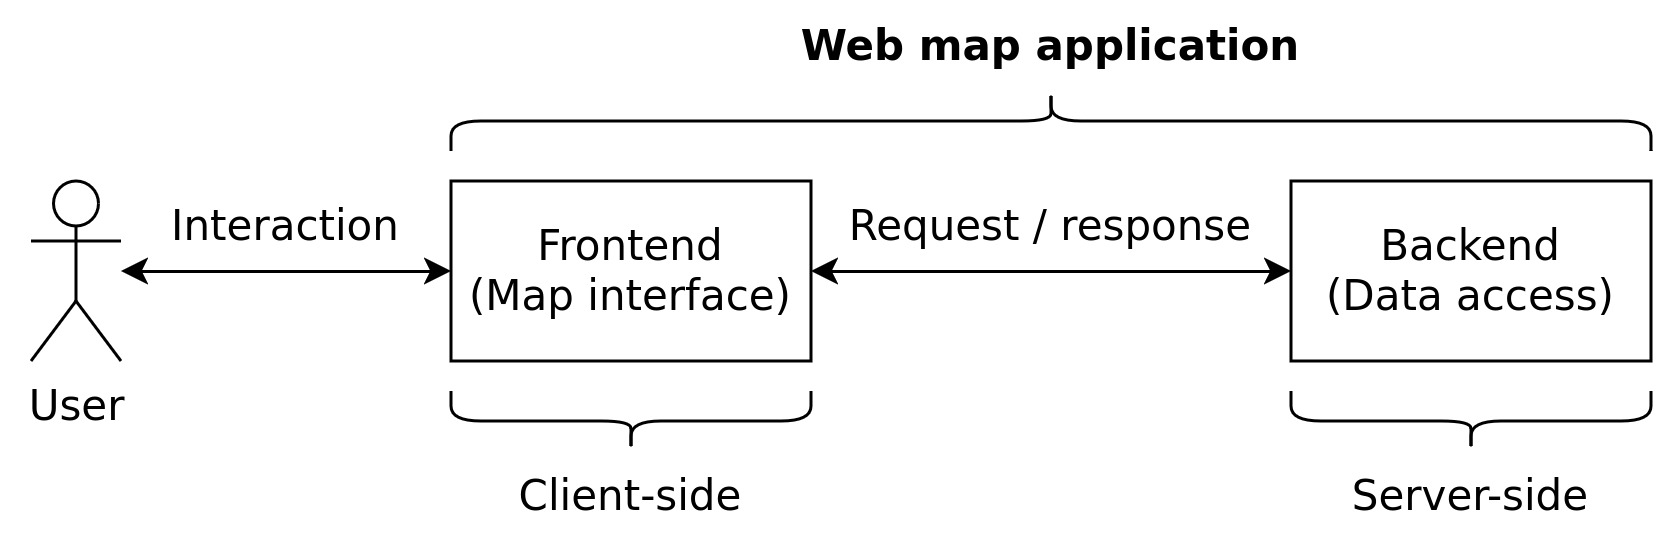
\includegraphics[width=\diagramwidth]{visual/figures/diagrams/web_map_app}
	\caption{
		A web map application like the one described above requires
		a frontend for providing the map interface
		and a backend for supplying the frontend with data to map.
	}
	\label{fig:web map app}
\end{figure}

I specified the software requirements at this quite non-detailed
level at first.
In accordance with the guideline of continuous adaptation,
\parencite{bec2001} I further focused them only as the application
and the study took shape.
However, to communicate the development and study process in an orderly manner,
and to motivate the design decisions I've made,
I present the requirements of the final application here.
Still, I should emphasize that the reality is not this linear.

The functional requirements specify the styles and modes of interaction,
as well as the set of operations a user can carry out with the map.
Firstly, the map should have two modes of interaction for selecting locations to be mapped.
These include clicking the map with a pointing device to produce a map of the clicked location,
and continuously changing the mapped location by moving the cursor over the map
(referred to as hovering).
This enables comparing two different levels of interactivity in the study:
clicking to produce static maps and hovering to produce
a responsive, \enquote{live},
representation of the accessibility under the cursor.
There should also be interface capabilities for selecting travel modes
and changing the mode of location selection.
To facilitate the exploration of the mapped area
at different points of focus and levels of detail,
the map should support panning and zooming the view.
The functional requirements are documented in table \ref{tab:functional requirements}.

For the quality attributes of the application,
performance is an essential consideration --
both in the sense of software performance
and the responsiveness of the application as perceived by the user.
This must be considered in both the front and backend of the application.
Quality attributes that are invisible to a user, but still vital,
are that the application can be maintained and deployed,
and that it can meet different real-world usage loads.
If these attributes were lacking,
the application would have little real value.
The \textit{deployment environment},
in other words the computing platform onto which the server-side of the application is deployed,
is the container orchestration platform \textit{Rahti} provided by the \presentacr{csc}.
Rahti is based on the \textit{OpenShift} platform,
which in turn runs on \textit{Kubernetes}.
Kubernetes is a container orchestration tool
that allows for declaratively managing clusters
of containerized applications and their accompanying services.
I mention these details because to the application they are constraints:
Both the front and backend implementations should be completely containerized,
and they both are deployed with the OpenShift flavour of Kubernetes.
Also, as is obvious by now,
the frontend of the application is constrained to running in a web browser.
For the nonfunctional requirements of the application,
see table \ref{tab:nonfunctional requirements}.

\begin{table}[H]
	\caption{The functional requirements of the map application}
	\label{tab:functional requirements}
	\centering
	\begin{tabular}{ | L{0.3\textwidth} | L{0.6\textwidth} | }
		\hline
		Requirement
		& Description
		\\
		\hline
		\hline
		Location selection by clicking
		& The user can click on a location and produce an accessibility map of that location.
		\\
		\hline
		Location selection by hovering
		& The user can hover their mouse over the map,
		and the map shows the accessibility of the location that is under the cursor,
		updating constantly as the cursor moves.
		\\
		\hline
		Toggling between modes of location selection
		& The user can toggle their mode of interaction by clicking:
		Clicking while hovering locks the map, clicking while the map is locked resumes hovering.
		\\
		\hline
		Interactive selection of travel mode
		& The user can choose the travel mode for which the travel times shown on the map are calculated.
		\\
		\hline
	\end{tabular}
\end{table}

\begin{table}[H]
	\caption{
		The nonfunctional requirements of the map application specify
		its desired qualities (\ref{tab:quality attributes}) and
		the constraints it must adhere to (\ref{tab:constraints}).
	}
	\label{tab:nonfunctional requirements}
	\begin{subtable}[h]{\textwidth}
		\caption{}
		\label{tab:quality attributes}
		\centering
		\begin{tabular}{ | L{0.2\textwidth} | L{0.7\textwidth} | }
			\hline
			\textbf{Category}
			& \textbf{Requirements}
			\\
			\hline
			\hline
			Performance
			& \tabitem Data serving speed allows for real-time interaction. \\
			& \tabitem Map rendering speed allows for real-time interaction. \\
			\hline
			Maintainability
			& \tabitem All components are as independent as possible. \\
			& \tabitem The codebase is versioned and documented. \\
			& \tabitem Deploying the application is reproducible. \\
			\hline
			Usability
			& \tabitem Visual feedback from user interaction is instantaneous. \\
			\hline
			Scalability
			& \tabitem The application is scalable to meet different usage loads. \\
			& \tabitem Different application components can be scaled independently. \\
			\hline
		\end{tabular}
	\end{subtable}
	\newline
	\newline  % https://tex.stackexchange.com/questions/38893/cant-generate-vertical-space-between-tables
	\newline
	\begin{subtable}[h]{\textwidth}
		\caption{}
		\label{tab:constraints}
		\centering
		\begin{tabular}{ | L{0.2\textwidth} | L{0.7\textwidth} | }
			\hline
			\textbf{Type of constraint}
			& \textbf{Description}
			\\
			\hline
			\hline
			Client-side platform
			& The frontend of the map application runs in a web browser.
			\\
			\hline
			Deployment environment
			& The front and backend are deployed in containers
			utilizing the OpenShift container platform.
			\\
			\hline
		\end{tabular}
	\end{subtable}
\end{table}



\subsubsection{Assessing data preprocessing approaches and preprocessing the TTM}

\label{sec:preprocessing}
% The need for preprocessing
% - what would raw data be like?
% - why as much as possible should be precalculated
% && the requirements preprocessing must satisfy
With initial testing,
it became obvious that
visualizing unprocessed \acrshort{ttm} data,
i.e. the complete 13000-cell grid of travel times for every location,
was not an option. This was due to two issues:
unresponsiveness of the map interface and the large file sizes.
Based on this,
I formed the hypothesis that either the file sizes
or the geometrical complexity of the data would be
the major factor limiting the responsiveness of the map,
i.e. the performance bottleneck.

So it was clear that
some type of preprocessing as well as simplification of the 
\acrshort{ttm} data was necessary --
both to test the hypothesis and to enable real-time interaction in the map.
The goal of assessing different approaches to data preprocessing, thus,
was to find the suitable level and types of simplification,
and to compare the effectiveness of different approaches.

When assessing the preprocessing approaches, I focused on:
\begin{itemize}
	\item The impact on file size, and thus on the speed of transferring data over internet.
	\item The impact on rendering speed of the map when mapping the data.
	\item The impact on the amount of information on the map,
	i.e. how much visual information is lost when a given approach is applied.
\end{itemize}

I assessed four types of preprocessing approaches:
\begin{itemize}
	\item Aggregation of travel time data into isochrone polygons \parenfig{isochrone intervals}
	\item Limiting the maximum travel time, i.e. the geographical extent of the results \parenfig{tt limits}
	\item Reducing the coordinate precision of geometries
	\item Minimizing files (simplifying GeoJSON structure, compression using gzip)
\end{itemize}

\begin{figure}[H]
	\centering
	\begin{subfigure}[b]{0.5\textwidth}
		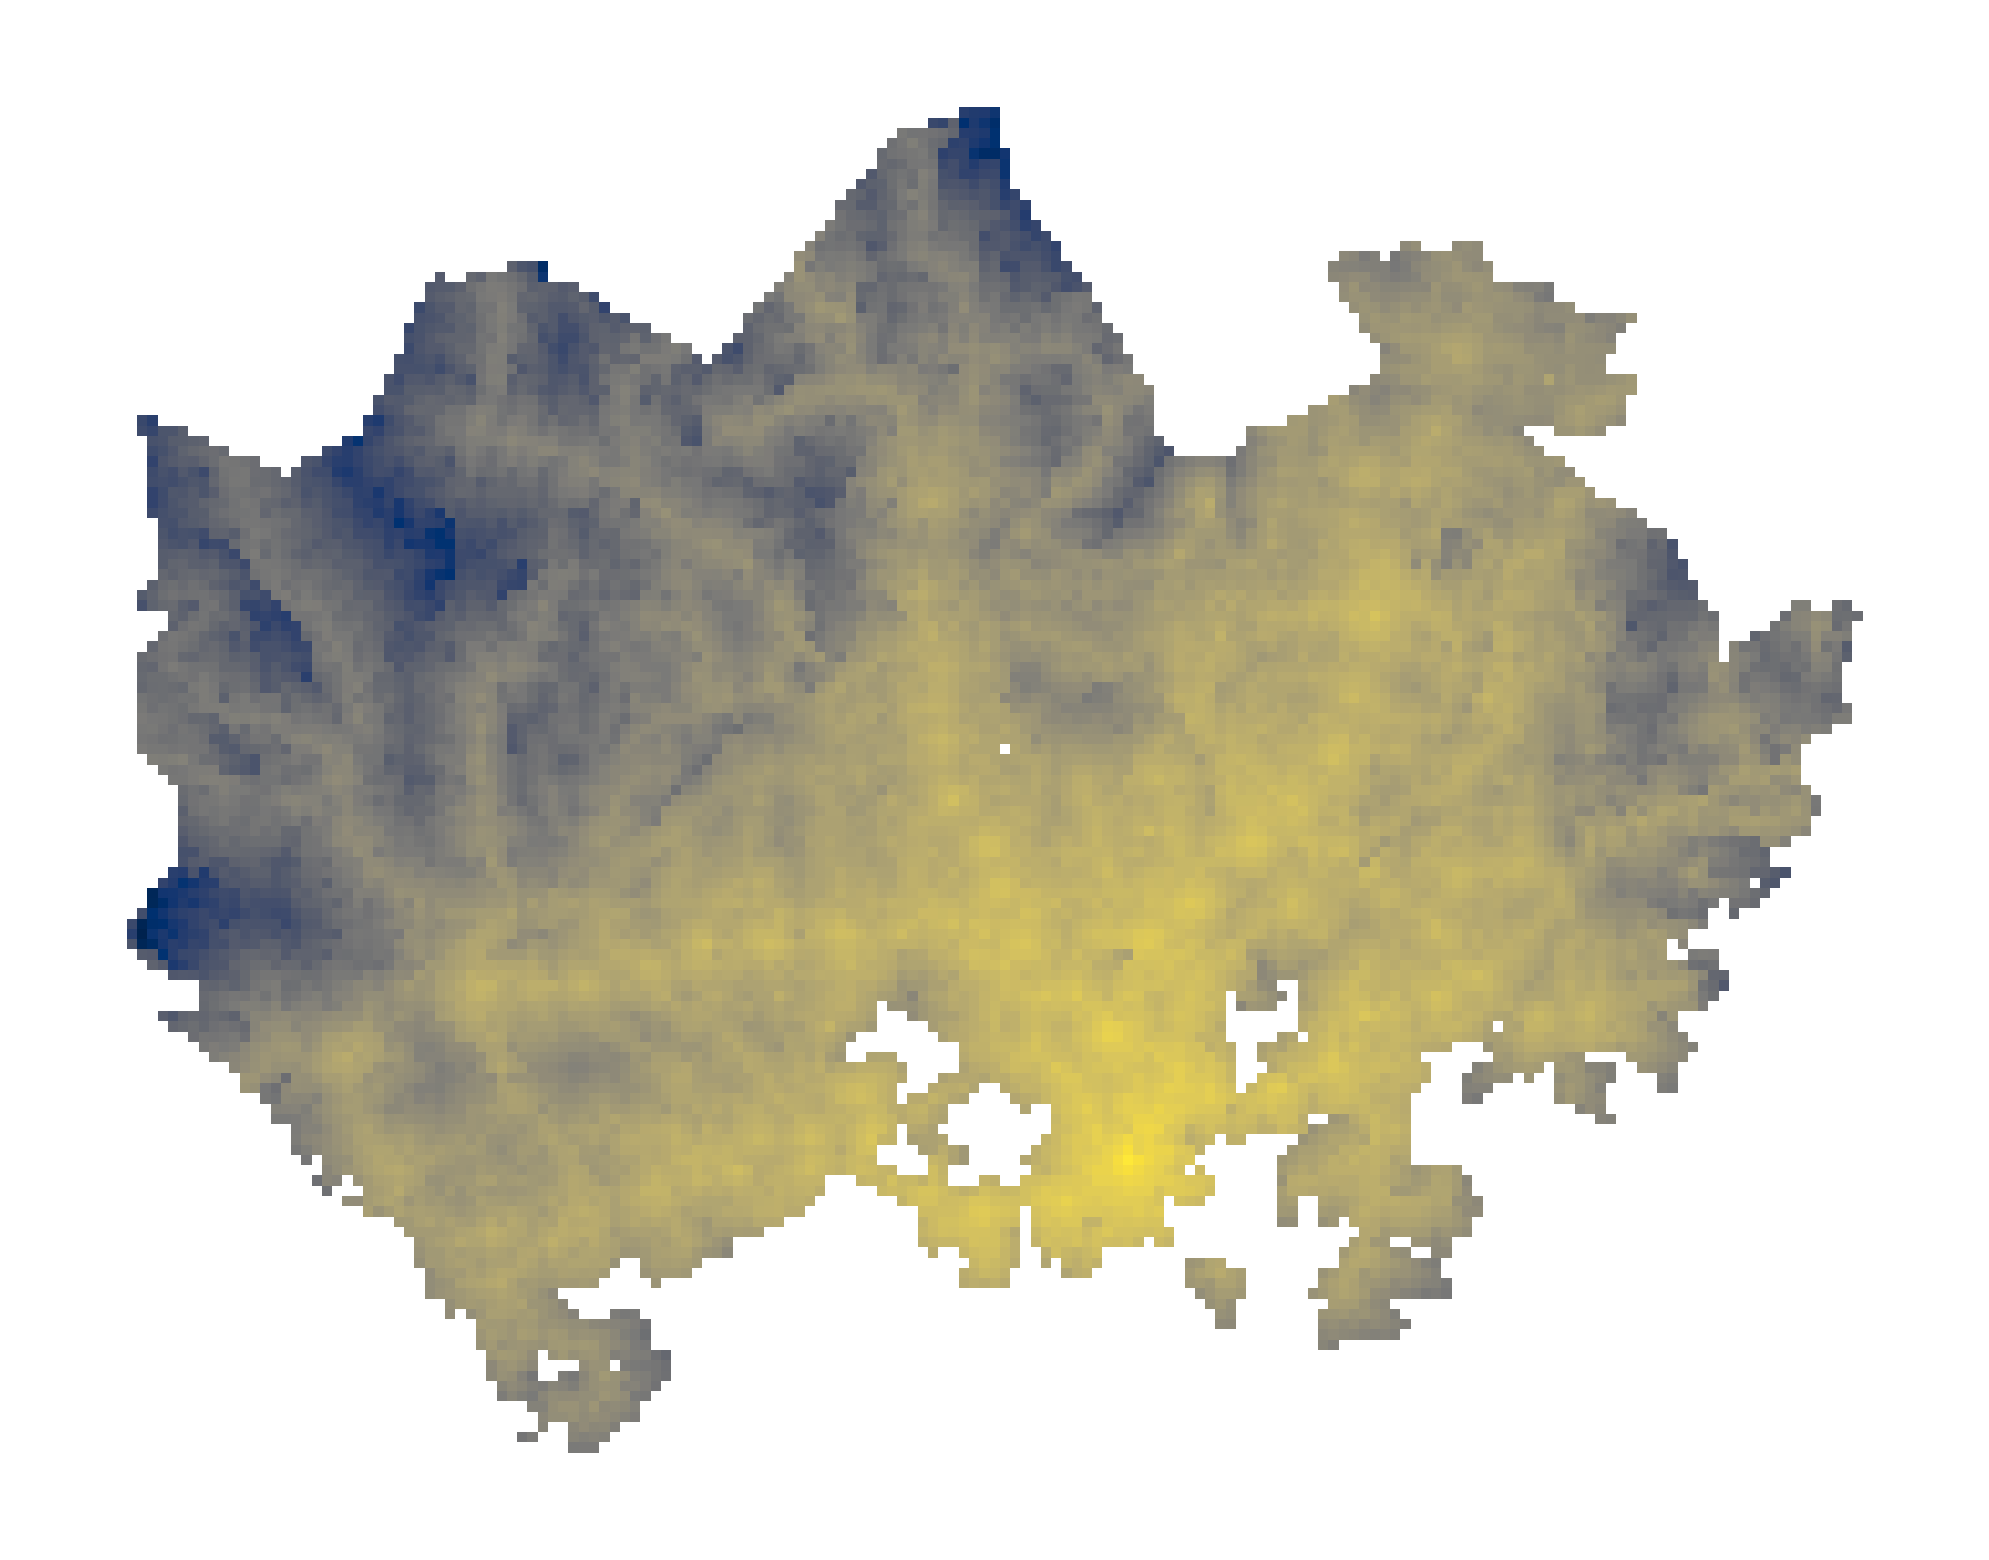
\includegraphics[width=\textwidth]{visual/figures/ttm/isochrone_interval_1}
		\caption{No isochrones}
		\label{fig:interval 1}
	\end{subfigure}%
	\hfill
	\begin{subfigure}[b]{0.5\textwidth}
		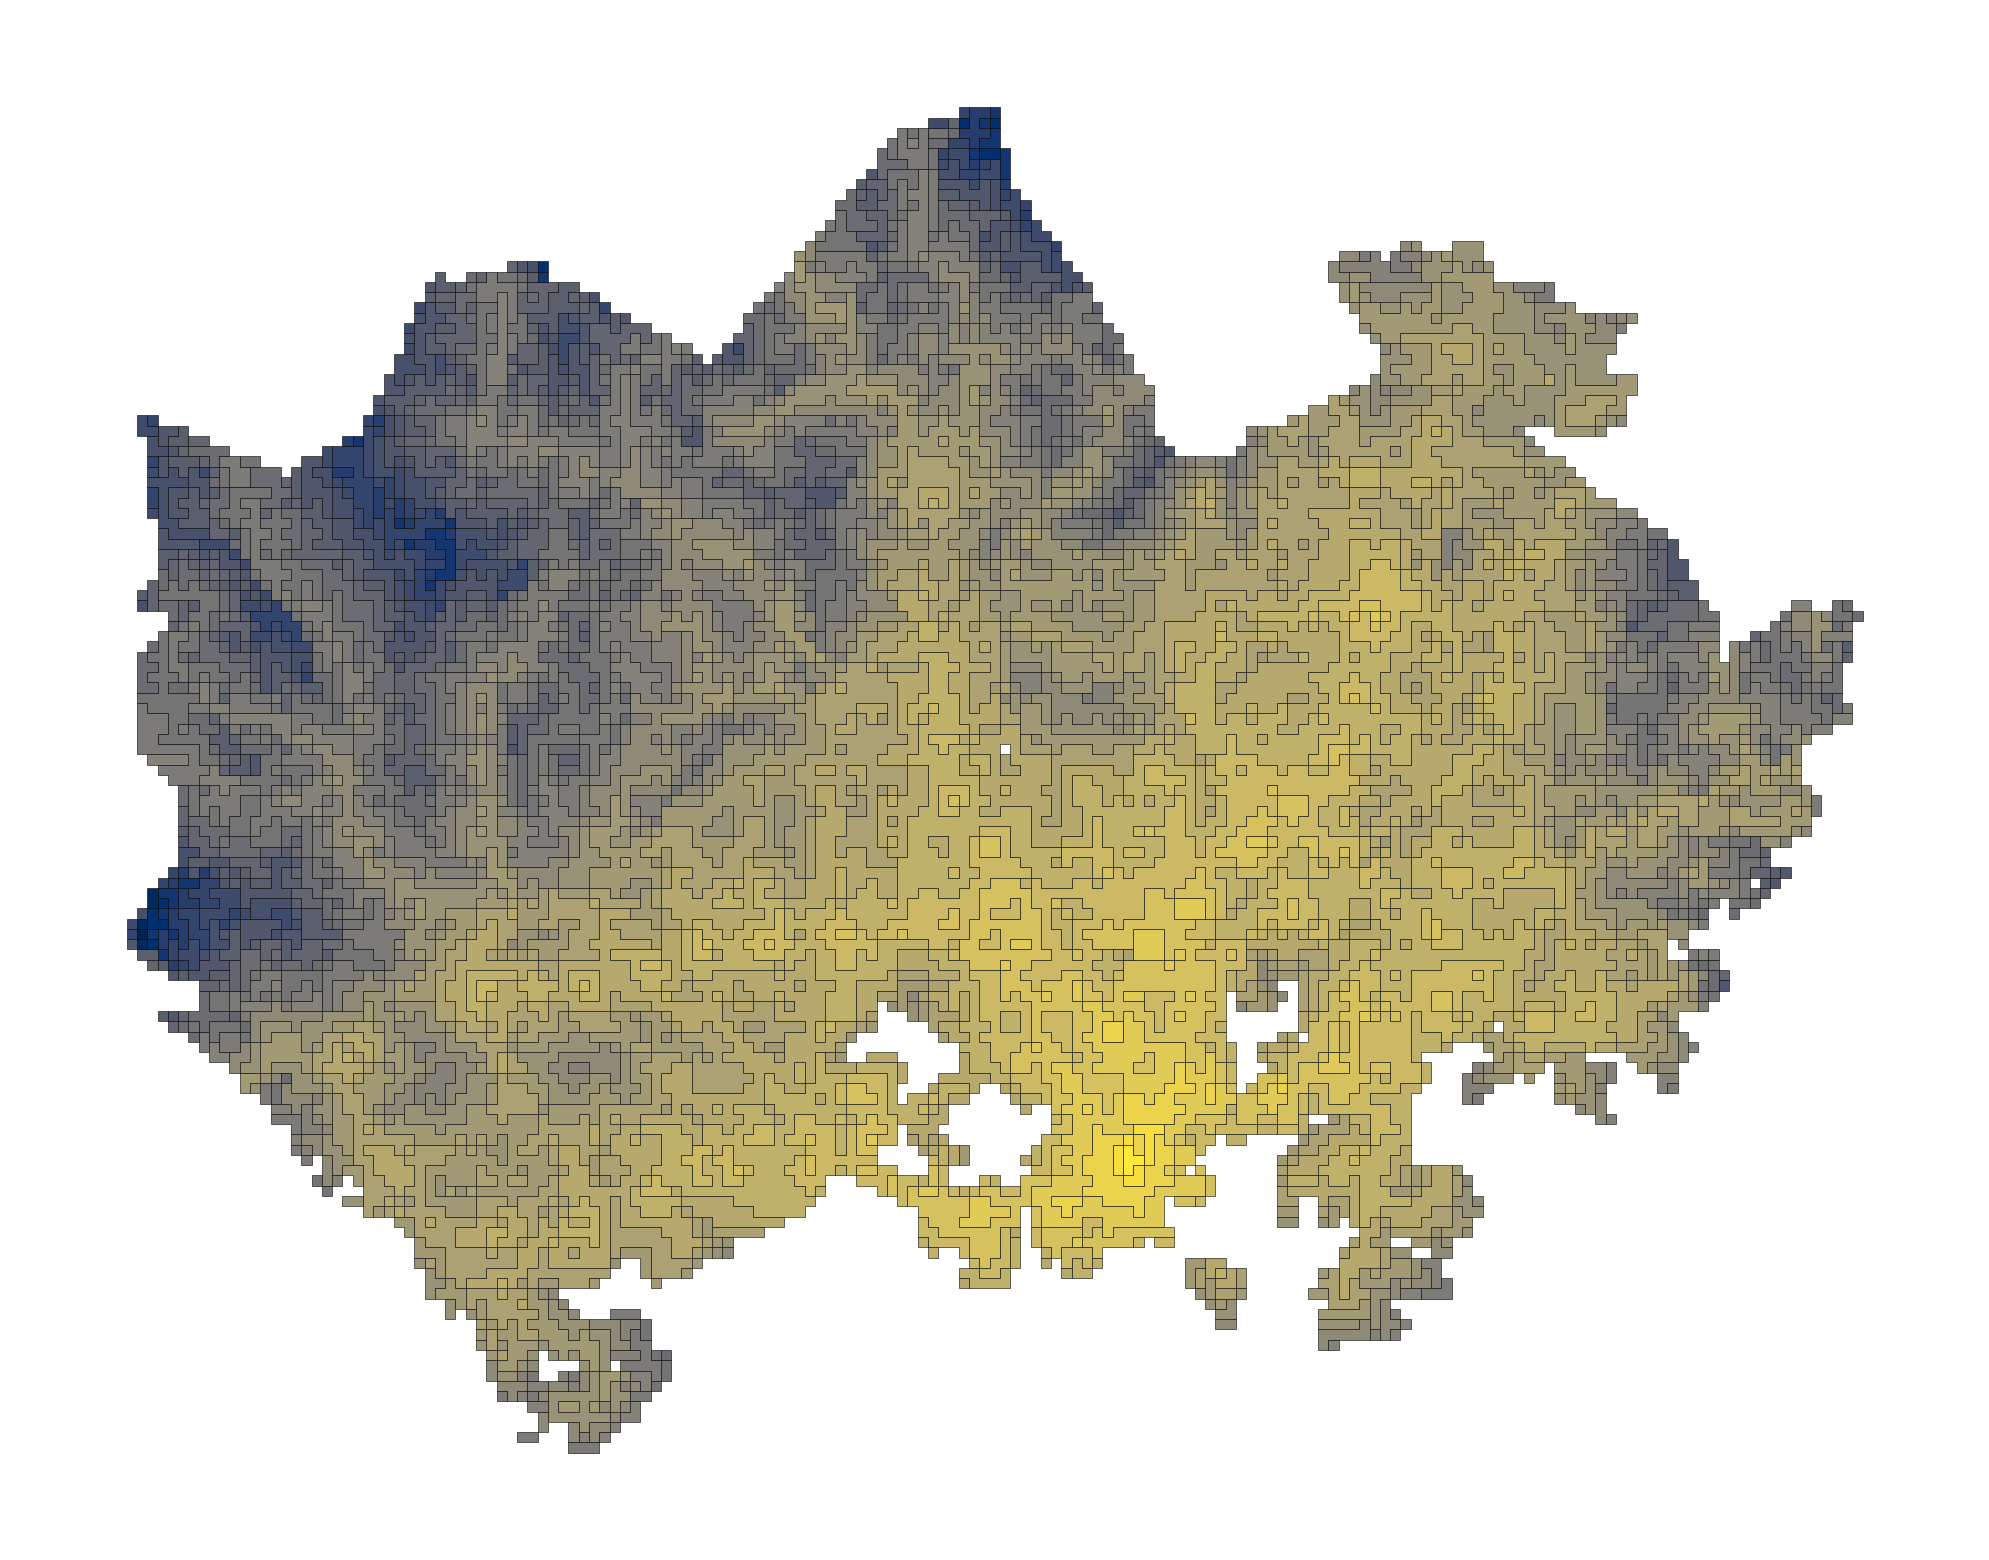
\includegraphics[width=\textwidth]{visual/figures/ttm/isochrone_interval_5}
		\caption{Isochrone interval = 5 minutes}
		\label{fig:interval 10}
	\end{subfigure}%
	\hfill
	\begin{subfigure}[b]{0.5\textwidth}
		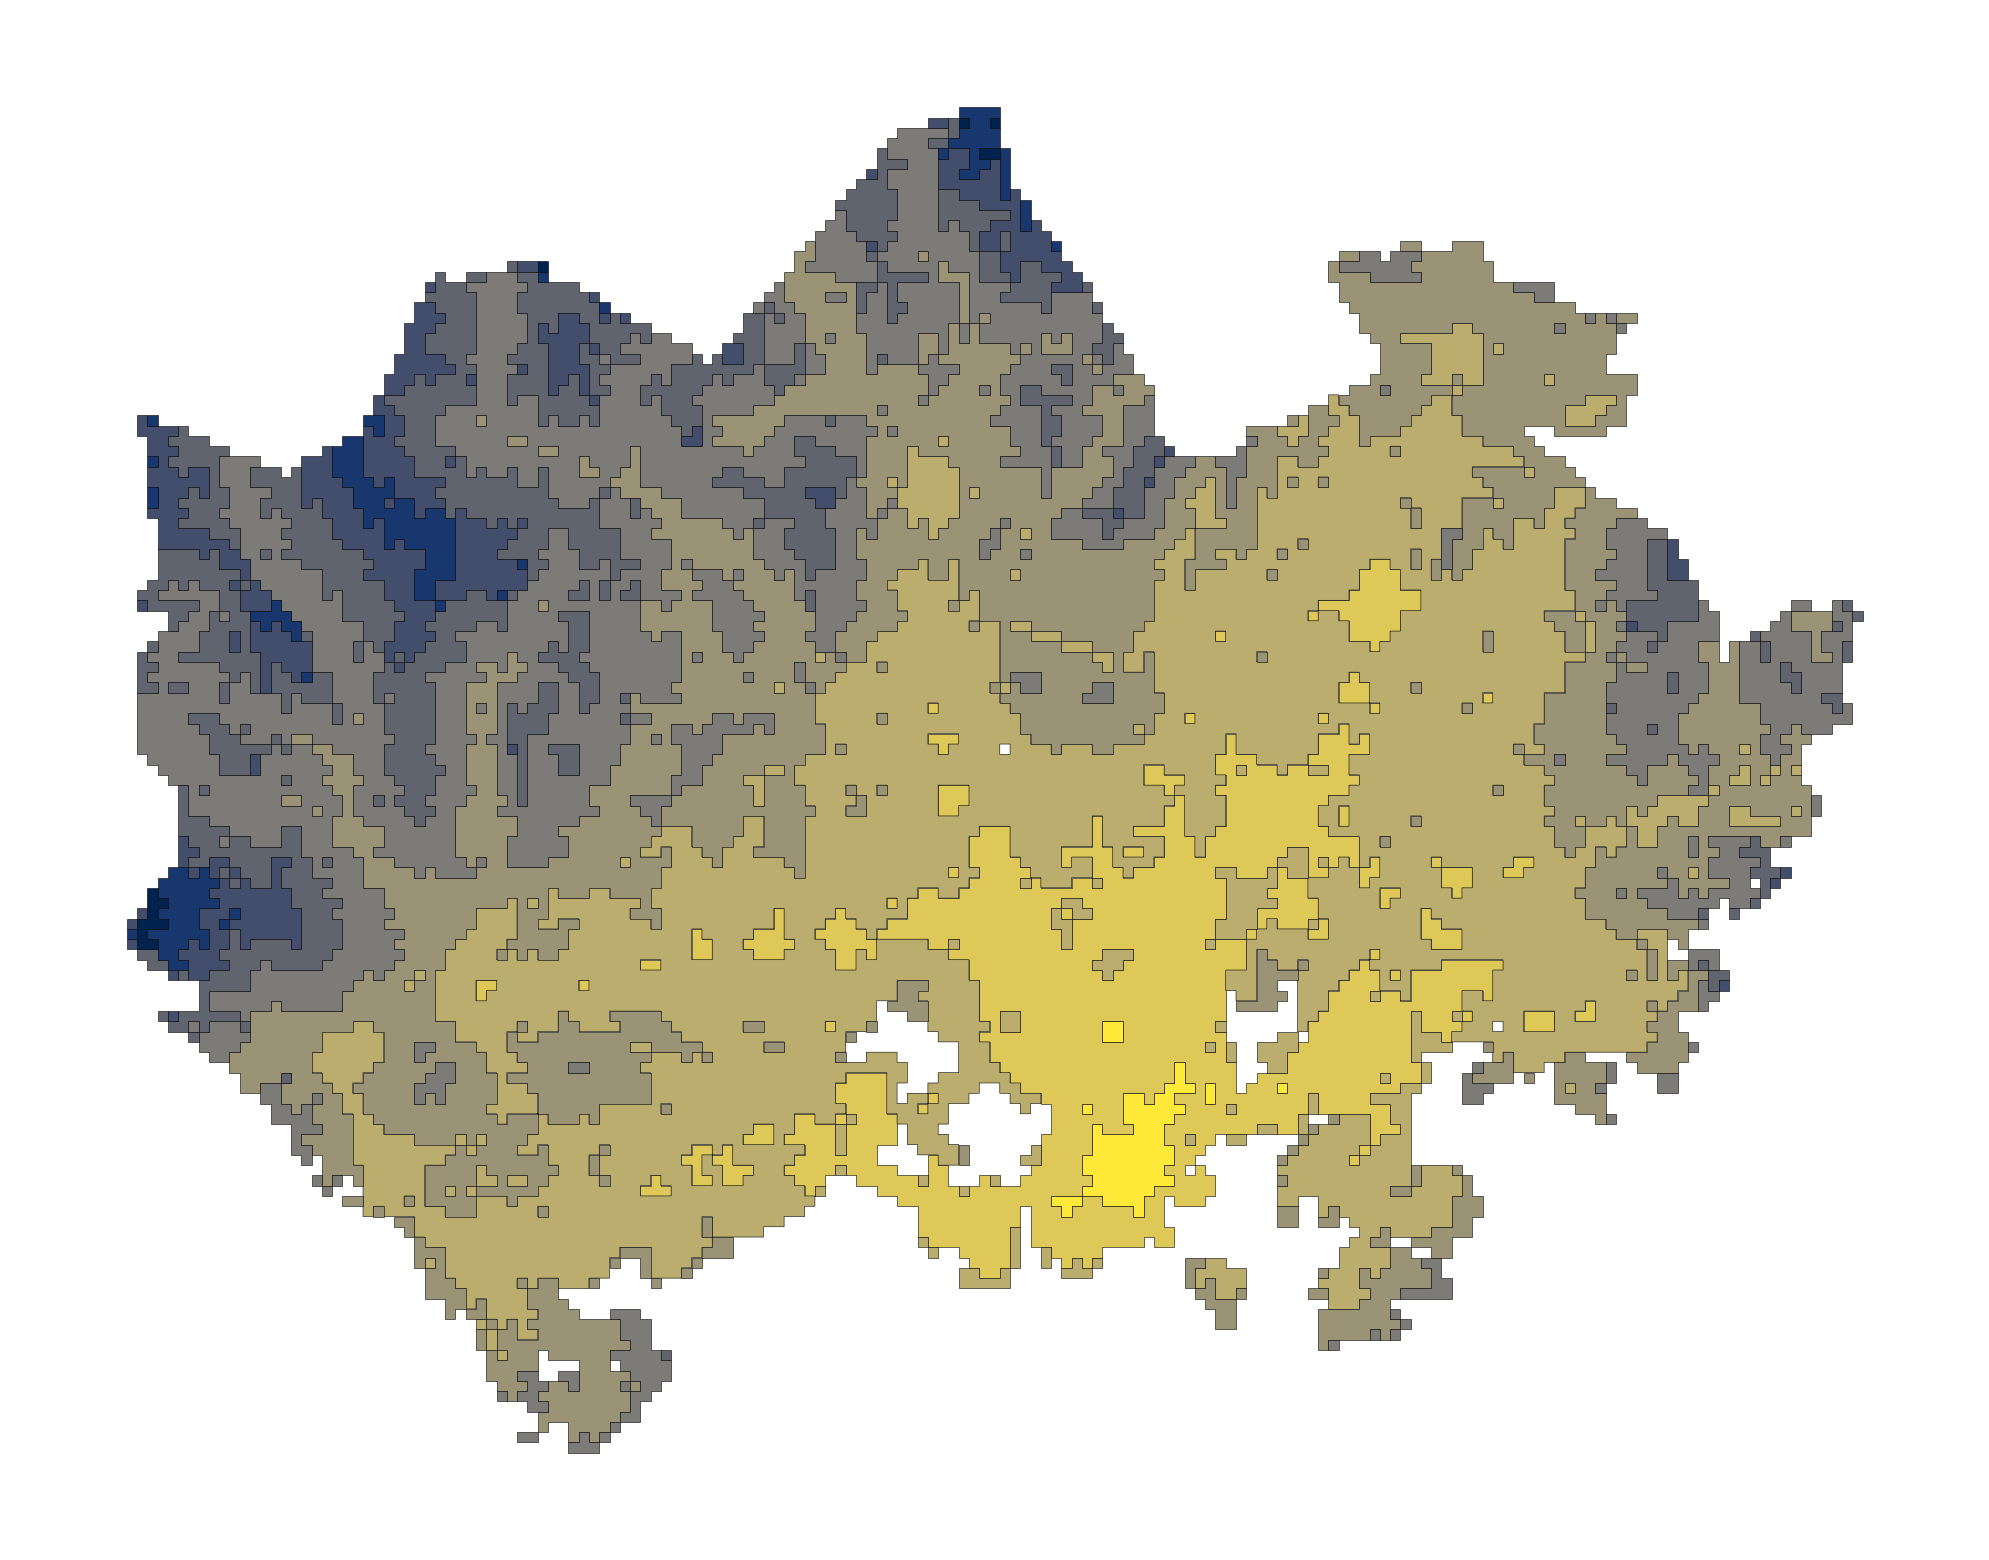
\includegraphics[width=\textwidth]{visual/figures/ttm/isochrone_interval_15}
		\caption{Isochrone interval = 15 minutes}
		\label{fig:interval 15}
	\end{subfigure}%
	\hfill
	\begin{subfigure}[b]{0.5\textwidth}
		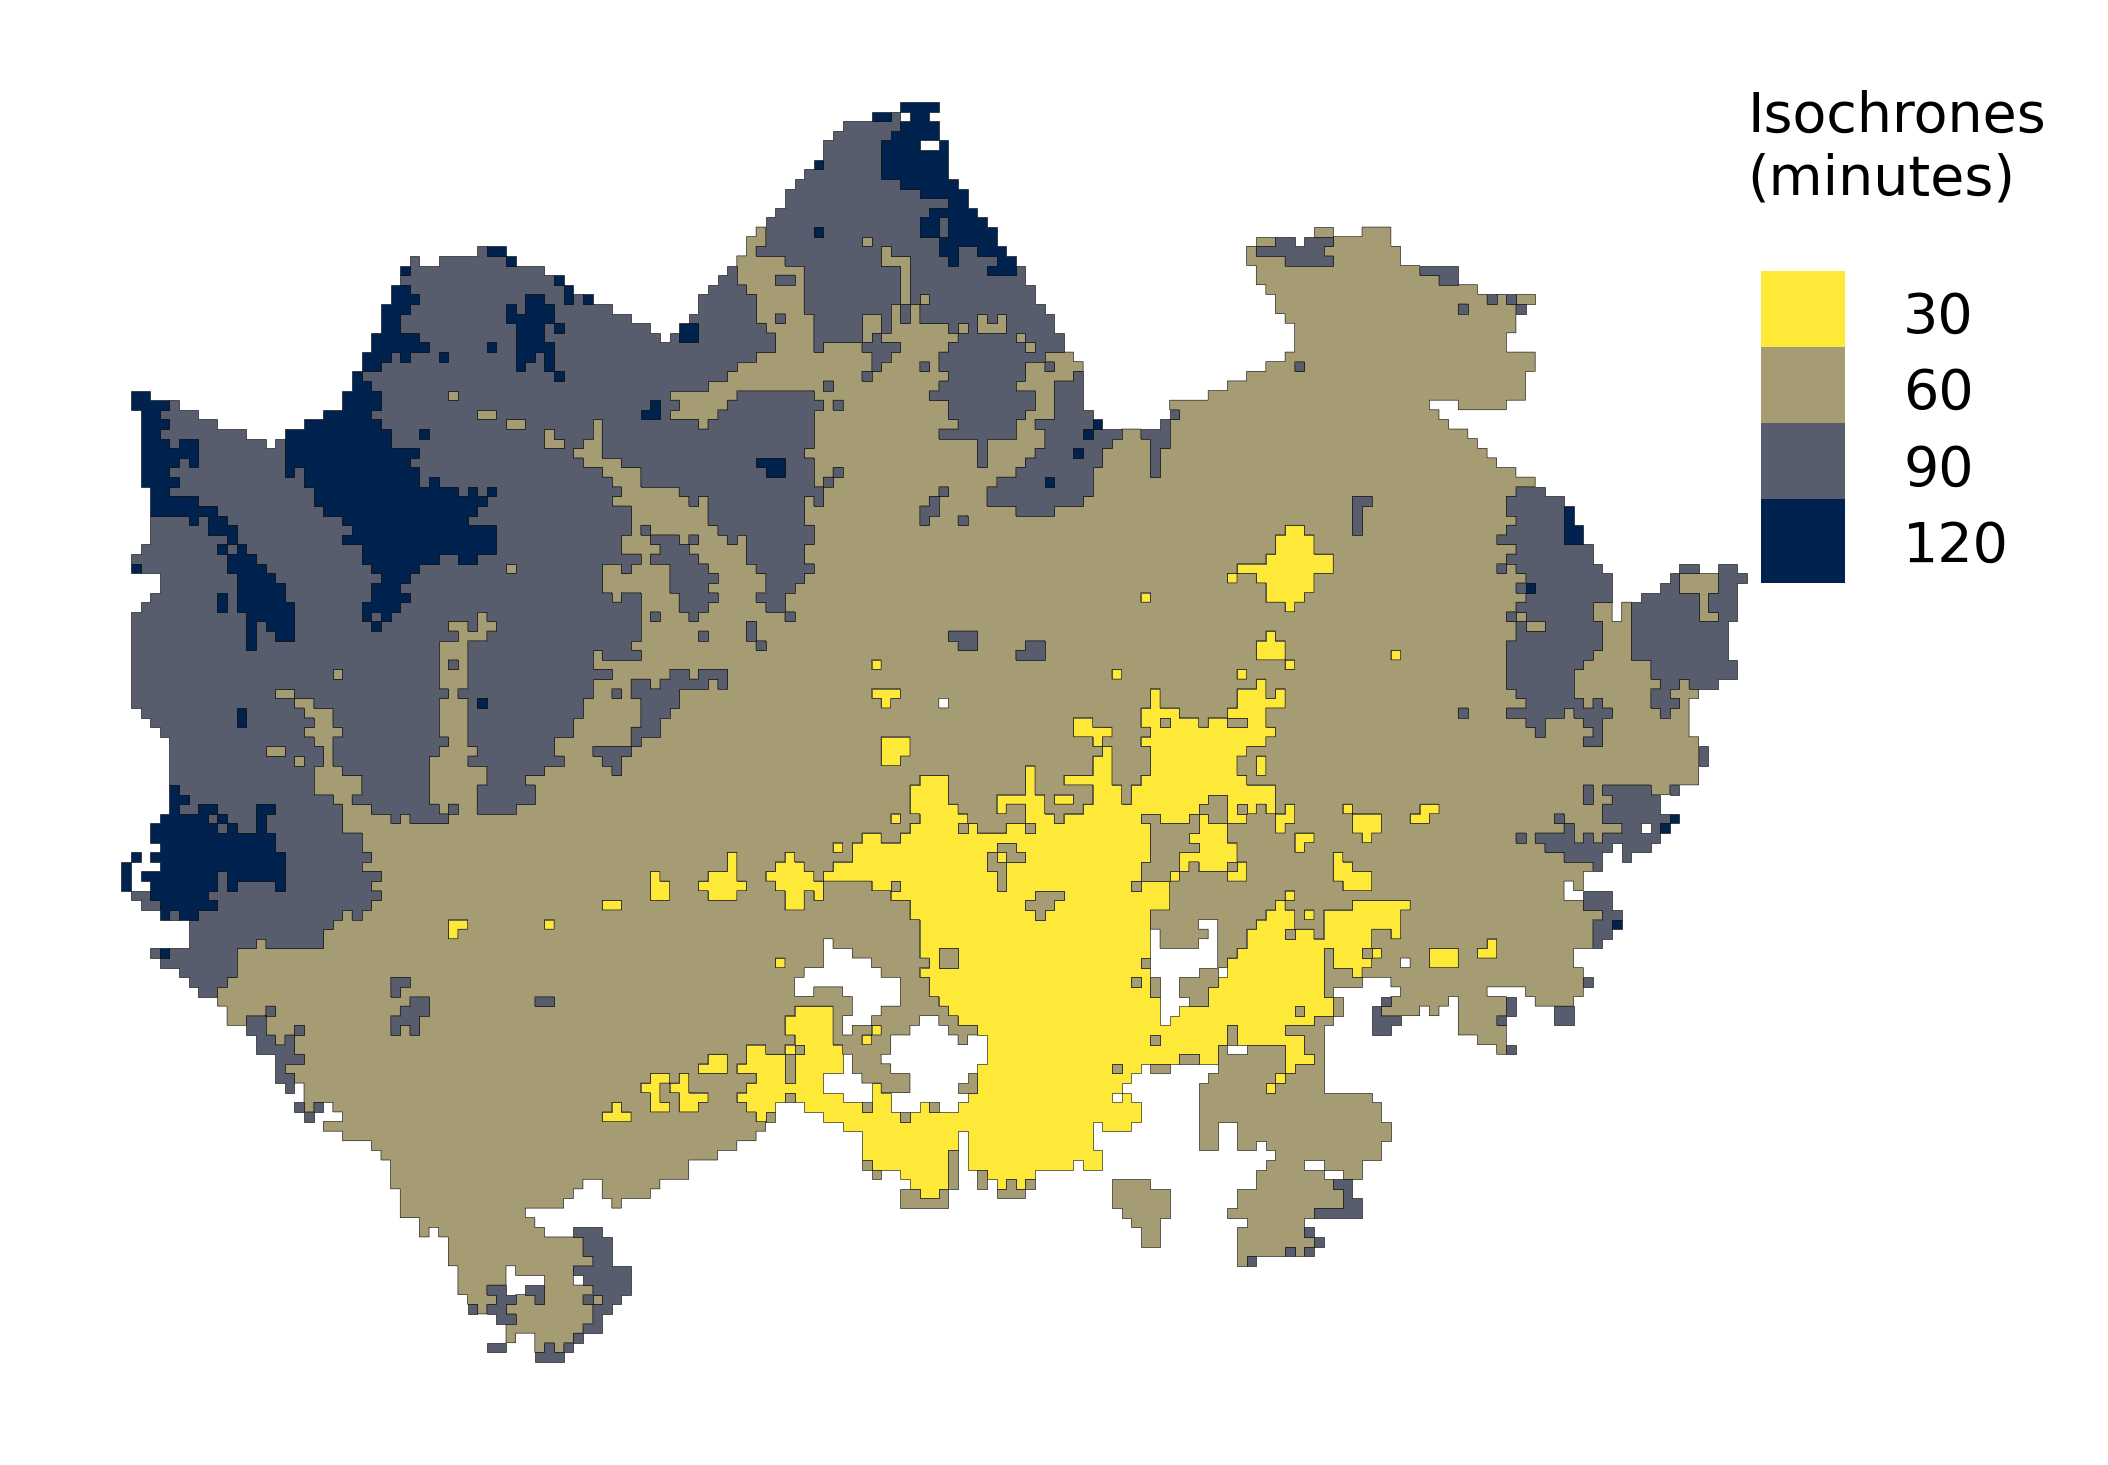
\includegraphics[width=\textwidth]{visual/figures/ttm/isochrone_interval_30}
		\caption{Isochrone interval = 30 minutes}
		\label{fig:interval 30}
	\end{subfigure}%
	\hfill
	\begin{subfigure}[b]{0.4\textwidth}
		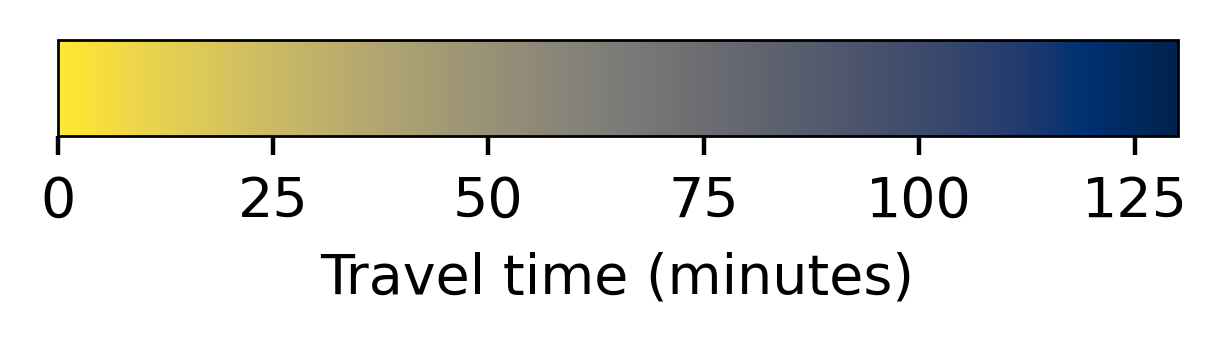
\includegraphics[width=\textwidth]{visual/figures/ttm/isochrone_cbar}
	\end{subfigure}%
	\caption{
		Travel time central to central Helsinki by public transport.
		Different levels of simplification can be achieved by
		aggregating travel times into isochrone polygons.
		Four examples are shown here, from no simplification
		to a highly simplified presentation
		(\ref{fig:interval 1}--\ref{fig:interval 30}).
	}
	\label{fig:isochrone intervals}
\end{figure}

\begin{figure}[H]
	\centering
	\begin{subfigure}[b]{0.5\textwidth}
		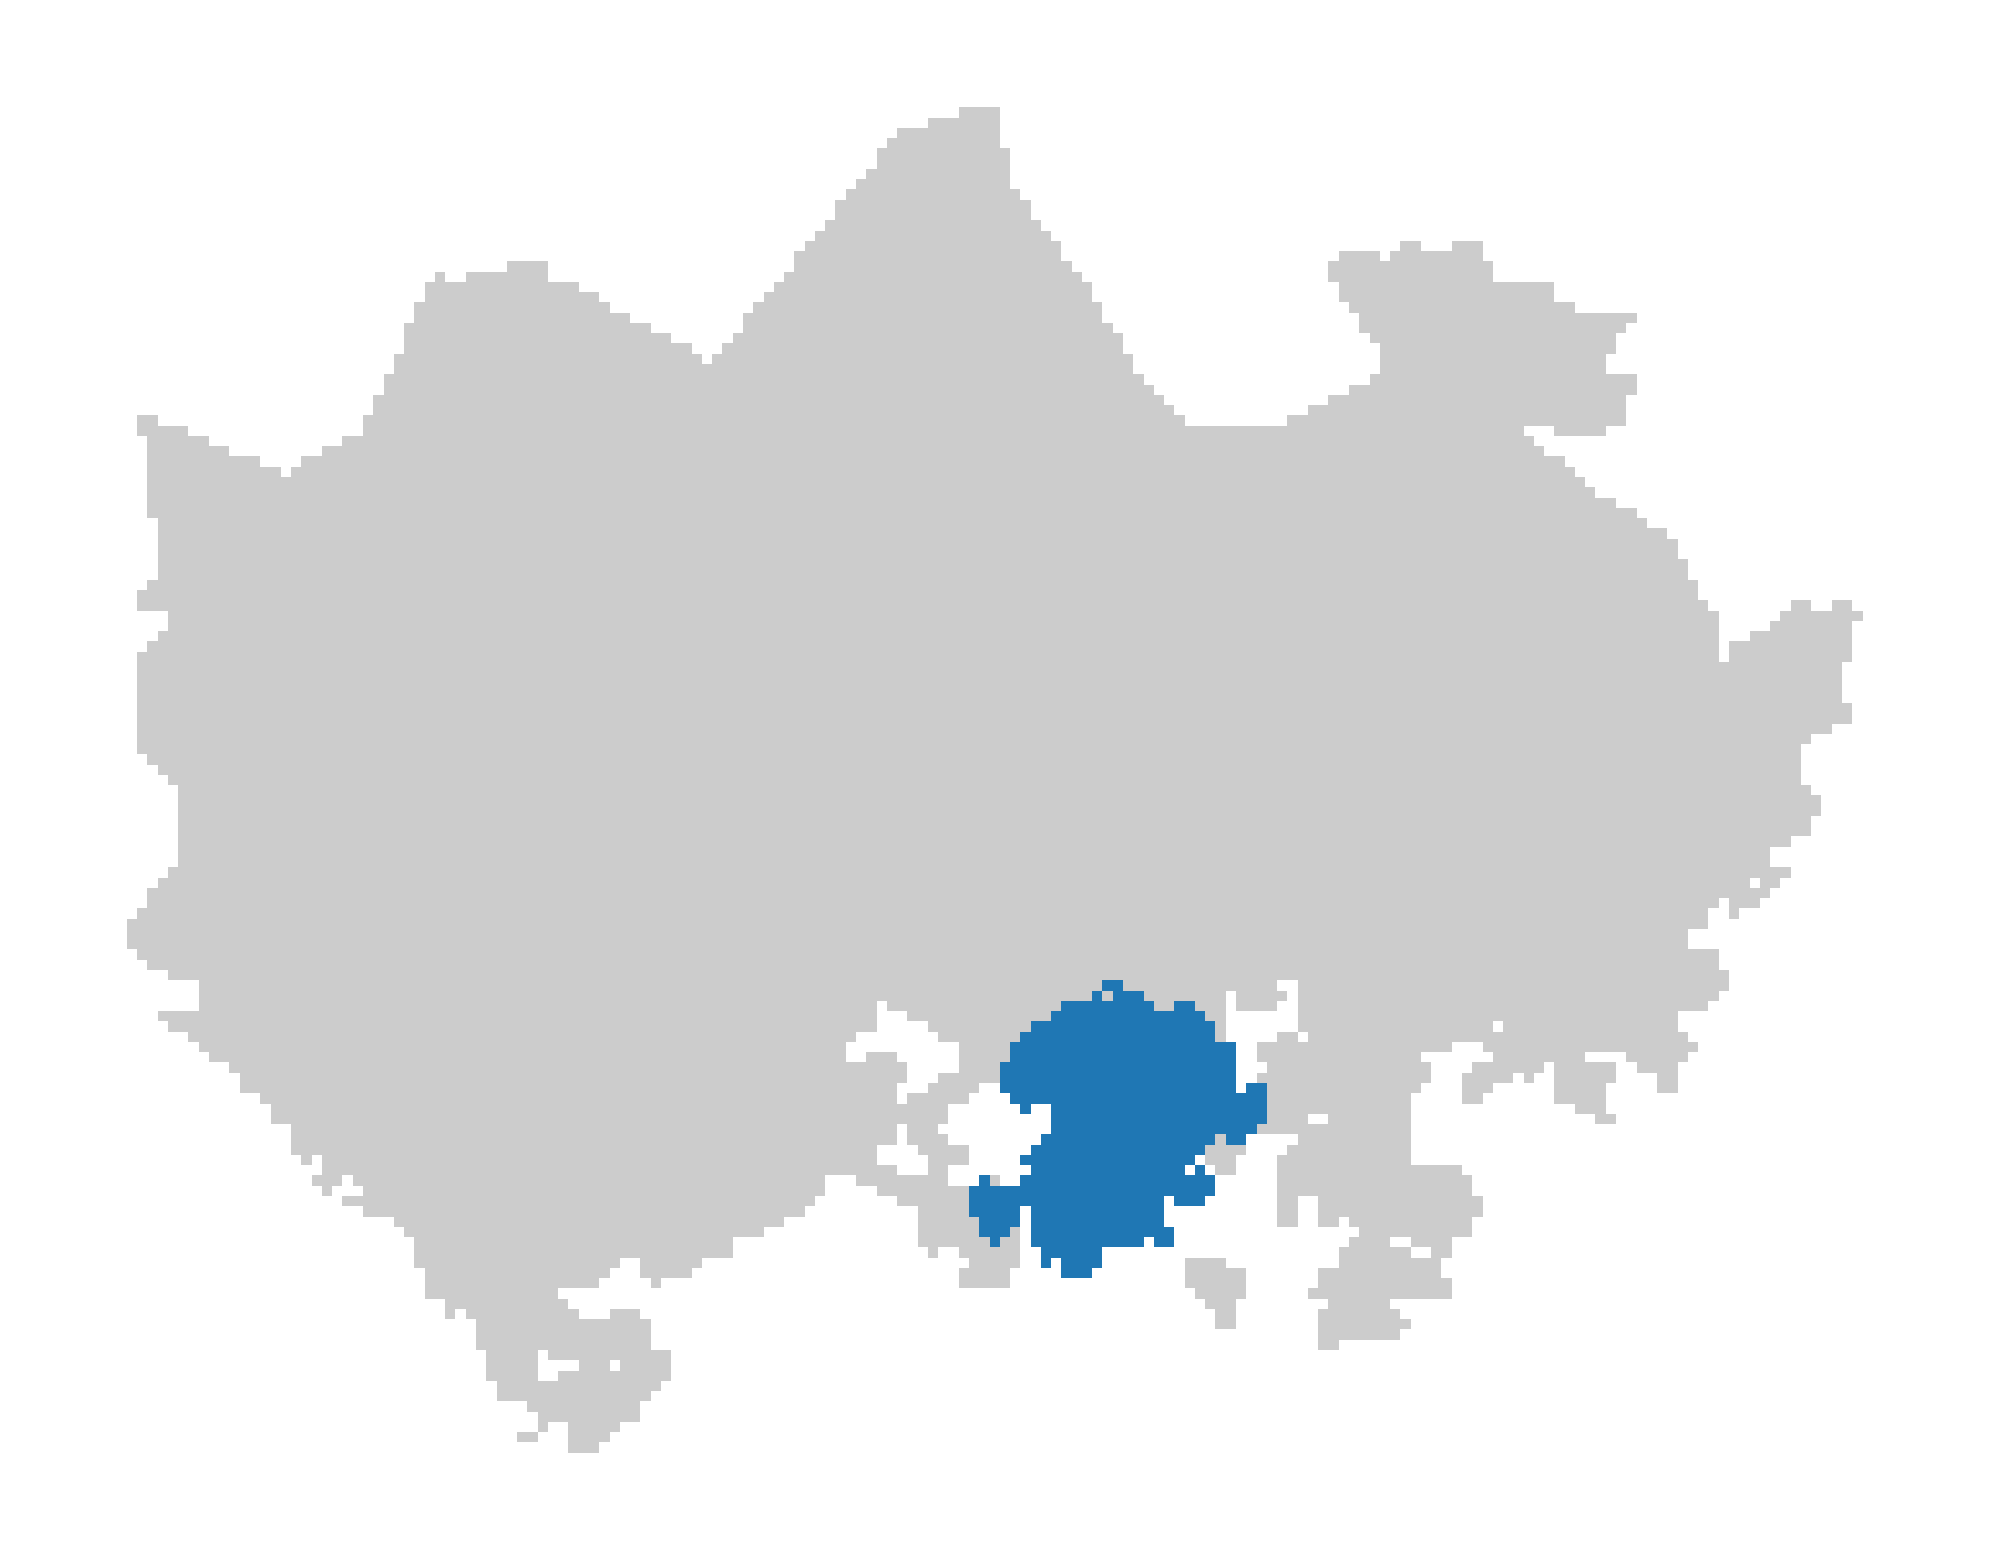
\includegraphics[width=\textwidth]{visual/figures/ttm/tt_limit_walk}
		\caption{Walk, 60-minute limit}
		\label{fig:limit walk}
	\end{subfigure}%
	\hfill
	\begin{subfigure}[b]{0.5\textwidth}
		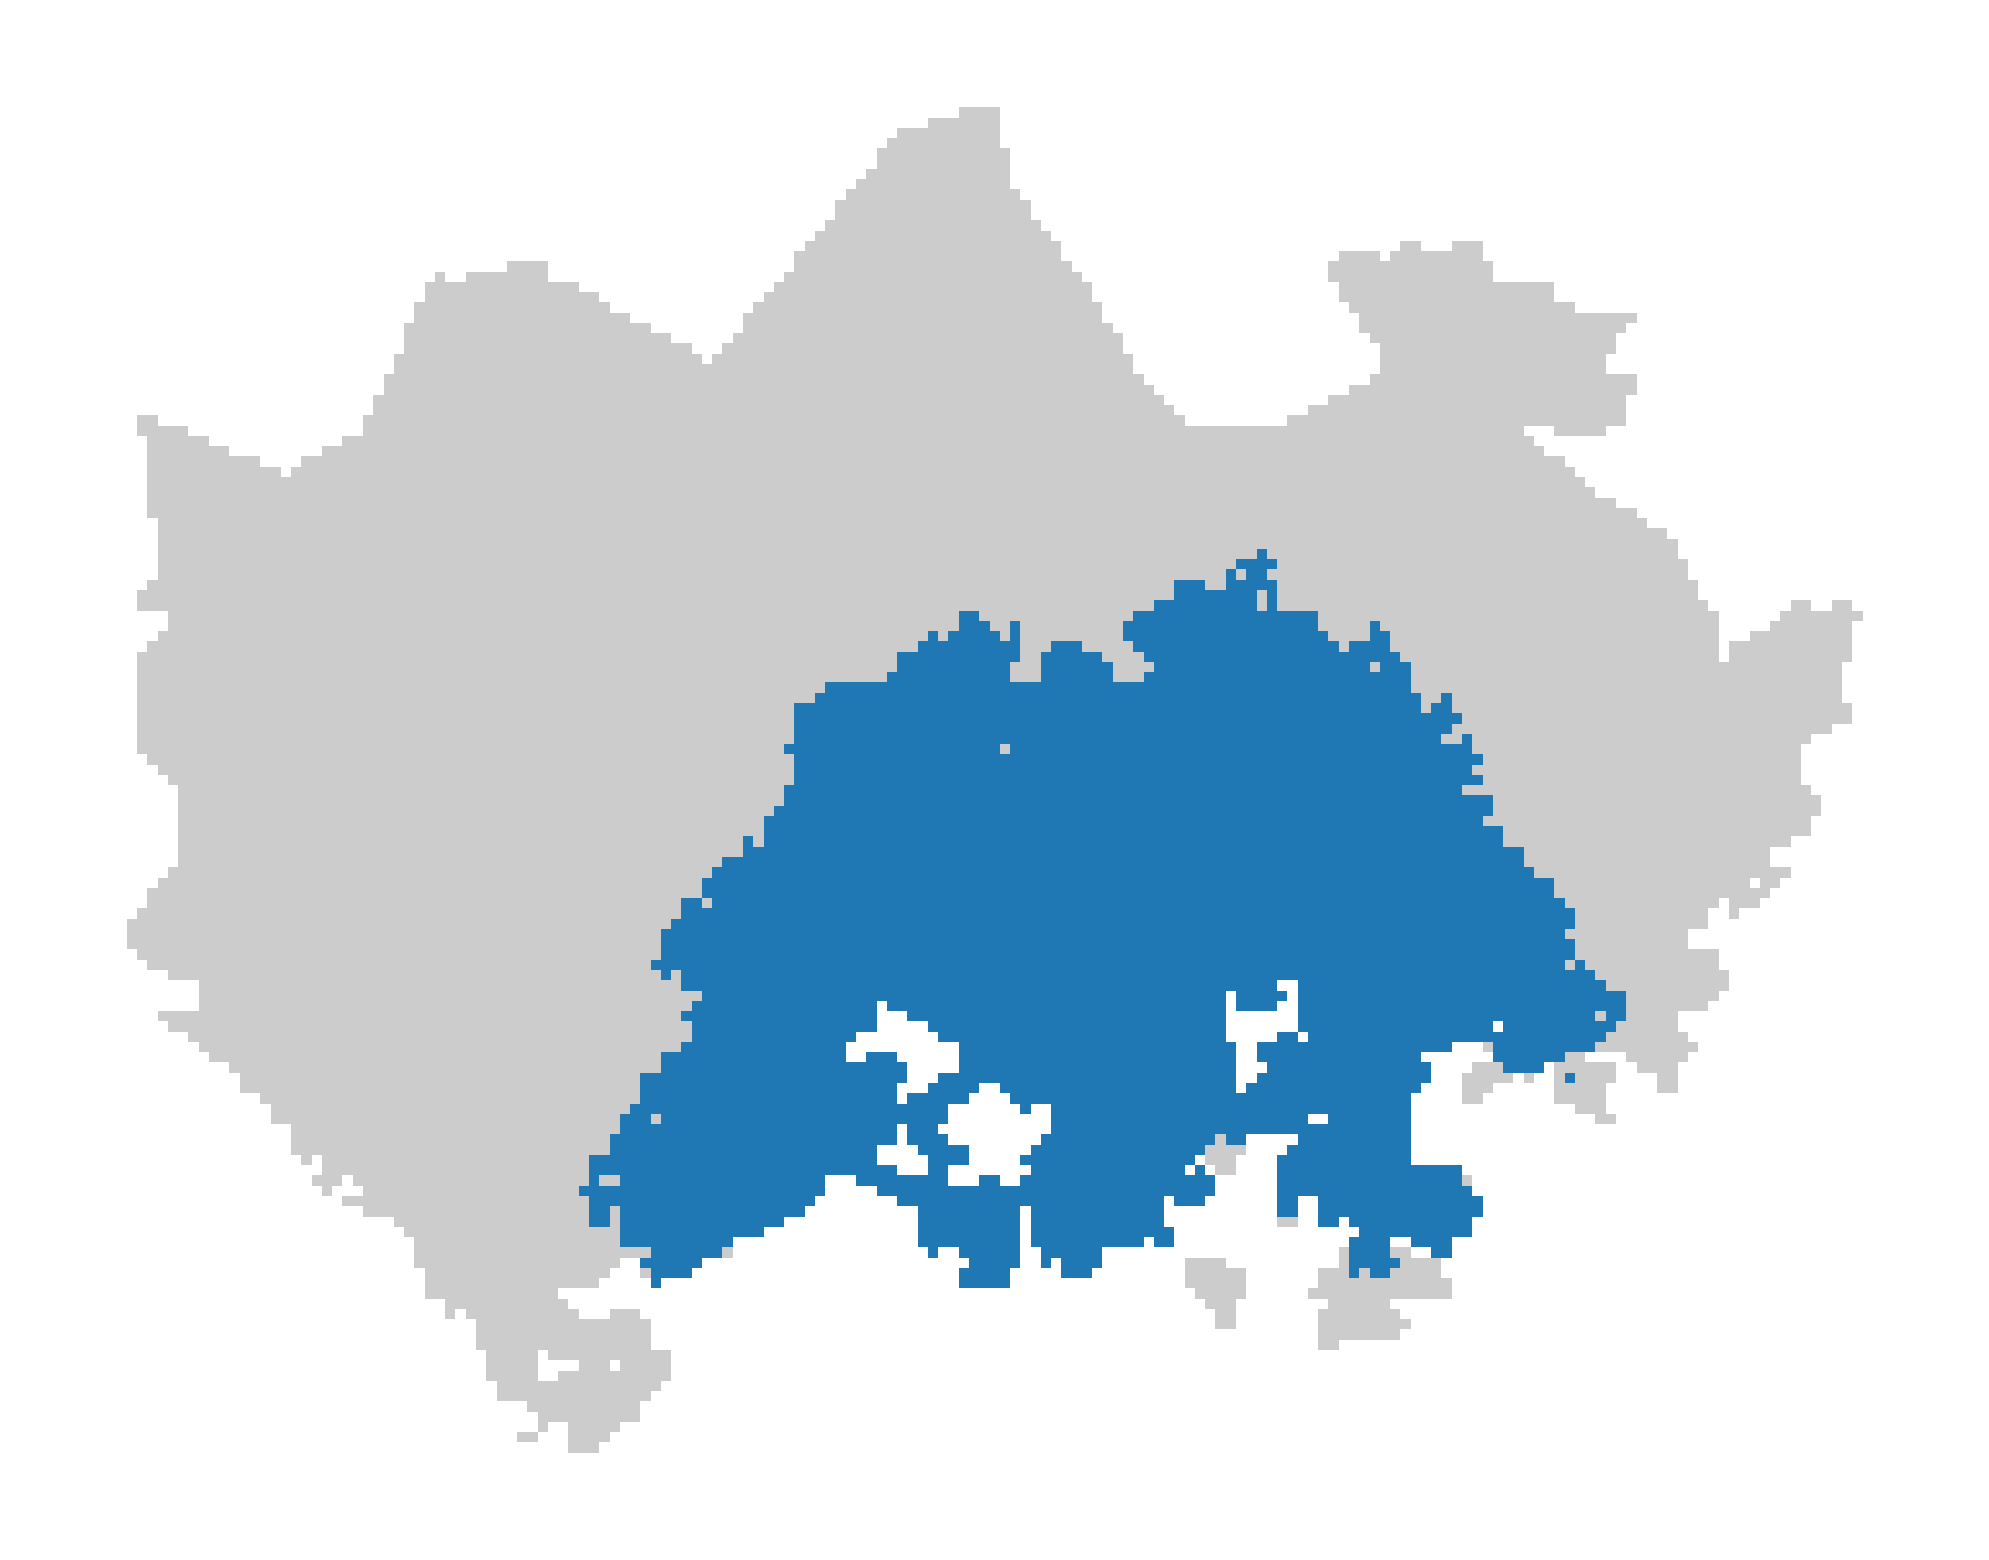
\includegraphics[width=\textwidth]{visual/figures/ttm/tt_limit_bike}
		\caption{Bike, 60-minute limit}
		\label{fig:limit bike}
	\end{subfigure}%
	\hfill
	\begin{subfigure}[b]{0.5\textwidth}
		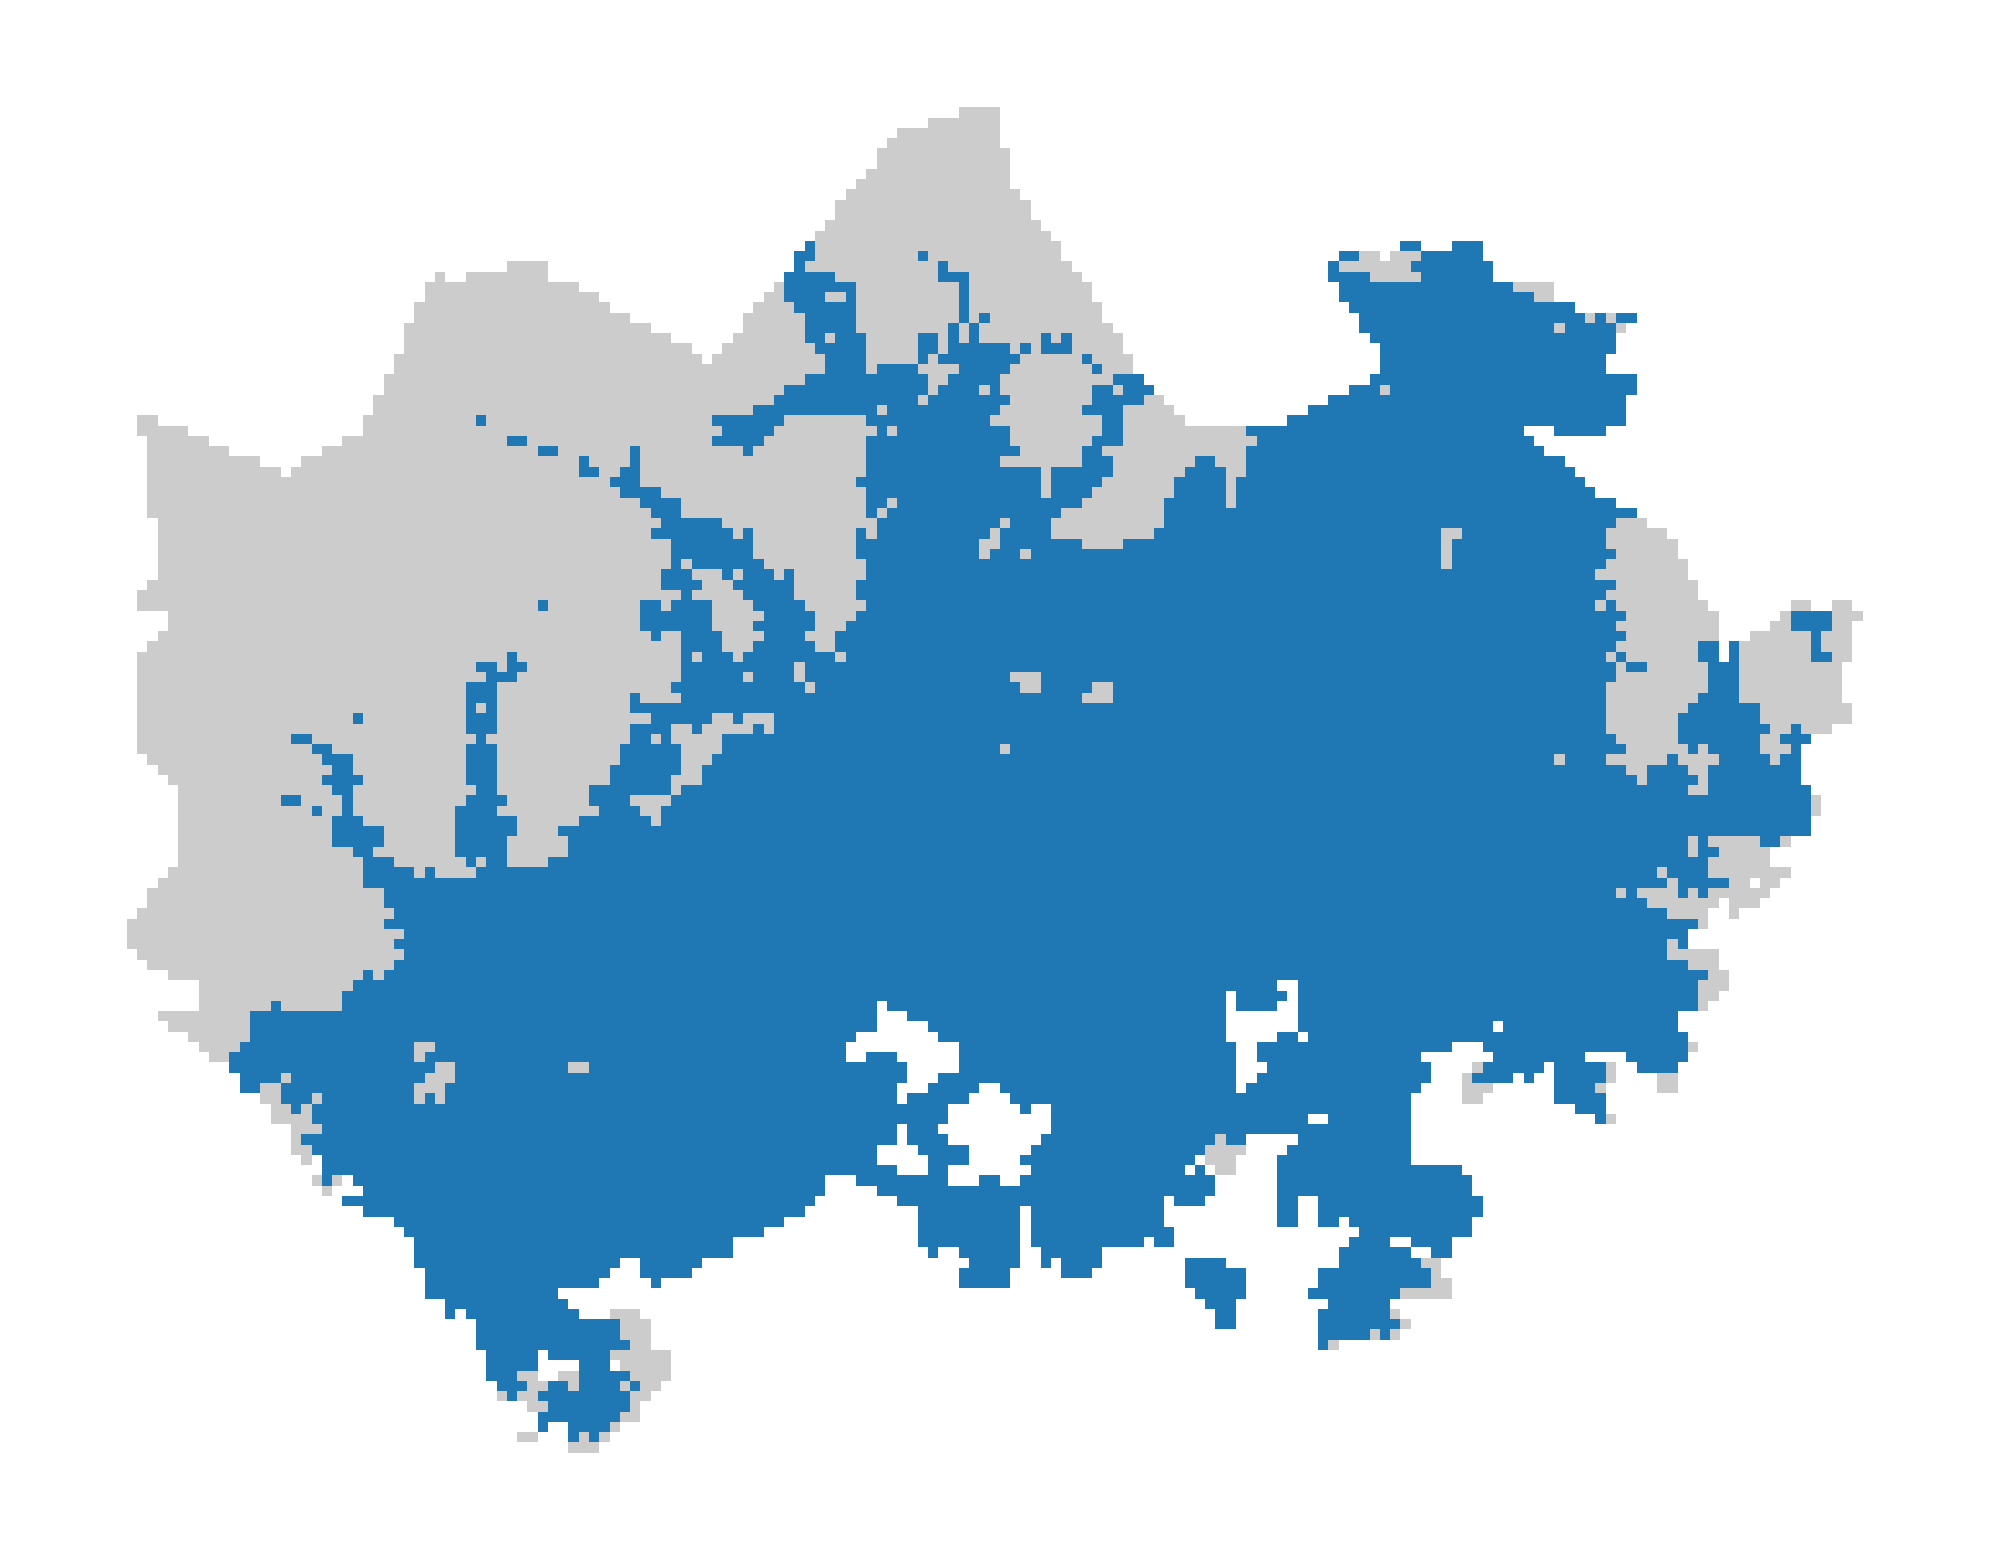
\includegraphics[width=\textwidth]{visual/figures/ttm/tt_limit_pt}
		\caption{Public transport, 60-minute limit}
		\label{fig:limit pt}
	\end{subfigure}%
	\hfill
	\begin{subfigure}[b]{0.5\textwidth}
		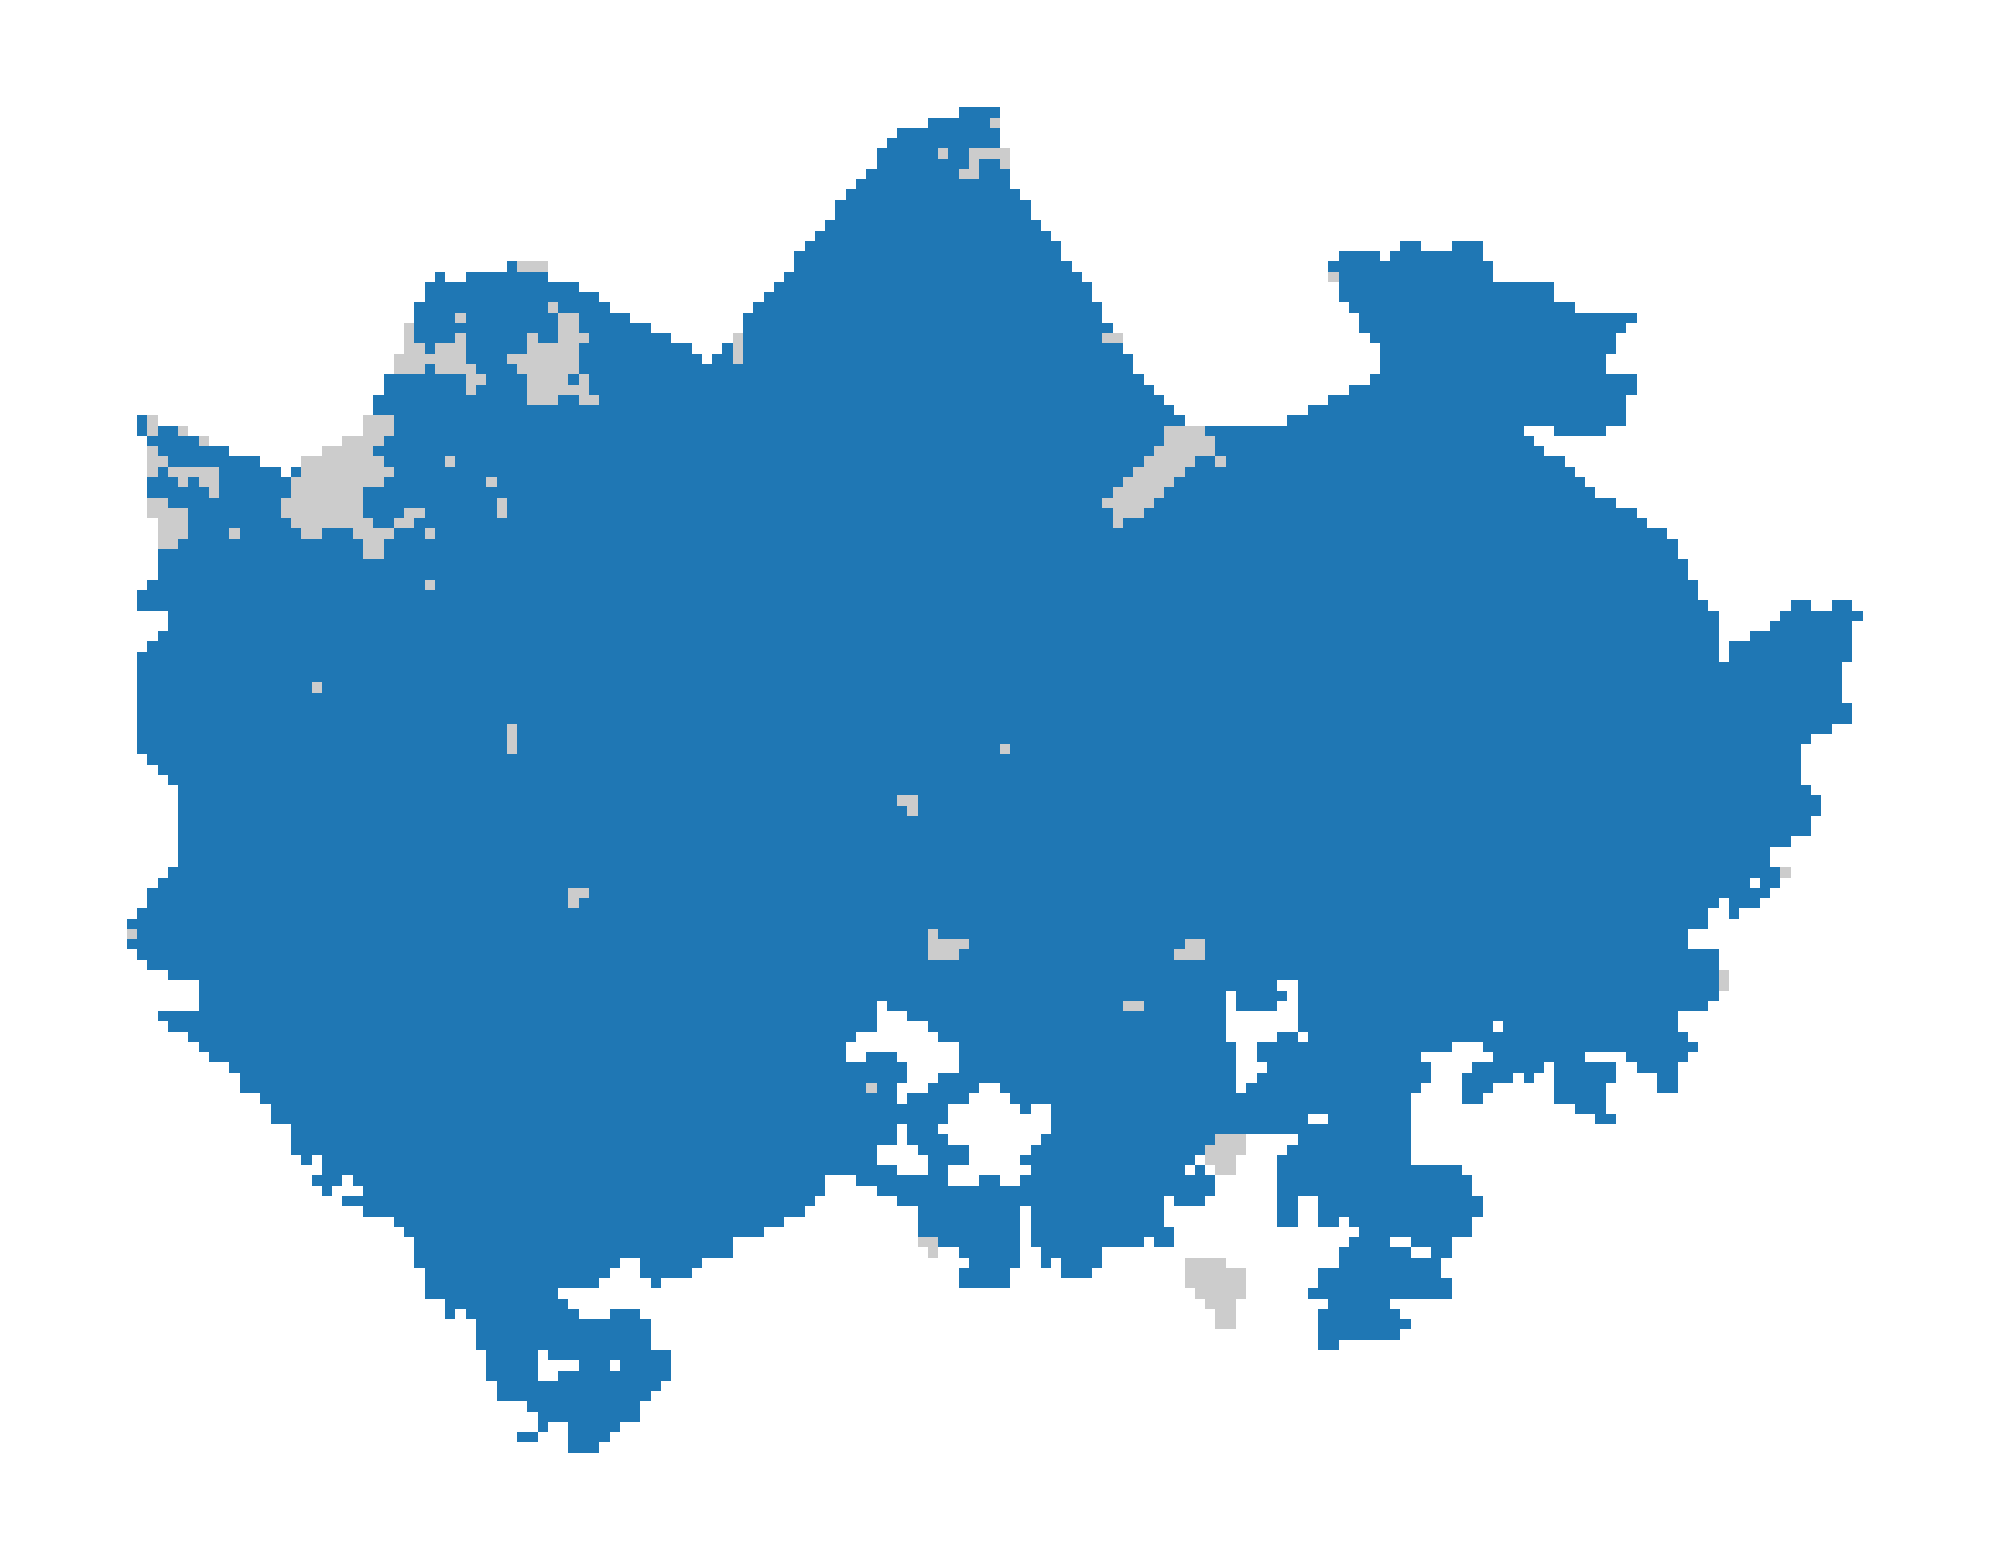
\includegraphics[width=\textwidth]{visual/figures/ttm/tt_limit_car}
		\caption{Car, 60-minute limit}
		\label{fig:limit car}
	\end{subfigure}%
	\hfill
	\begin{subfigure}[b]{0.55\textwidth}
		
\includegraphics[width=\textwidth]{visual/figures/ttm/tt_limit_legend}
	\end{subfigure}%
	\caption{
		The area where central Helsinki is reachable within an hour of travel.
		In general, limiting the maximum travel time reduces the spatial extent of data,
		more drastically for walking and biking (\ref{fig:limit walk}--\ref{fig:limit bike}),
		and less so for public transport and car (\ref{fig:limit pt}--\ref{fig:limit car}).
	}
	\label{fig:tt limits}
\end{figure}

To enable the assessment
I constructed a modular preprocessing pipeline
(figure \ref{fig:preprocessing}).
By modular I mean that,
while the complete pipeline applies all preprocessing approaches,
the design allows for isolated testing of the
different components of the pipeline, with different parameters.
I used Python \parencite{python} for implementing most of the preprocessing pipeline,
relying on the GeoPandas \parencite{jor2024} library for all spatial operations.
In addition, I carried out file compression with
the standard GNU utilities bash \parencite{bash} and gzip \parencite{gzip}.
Gzip compression was the natural choice,
as it is the ubiquitous approach to file compression on the web. 
I tested the preprocessing approaches on
a randomly picked set of 100 locations in the \acrshort{ttm},
for each travel mode.
A random sample of locations is necessary when either
isochrone aggregation or a travel time limitation is applied,
since in these cases the complexity of the resulting
data varies greatly based on location.

\begin{figure}[H]
	\centering
	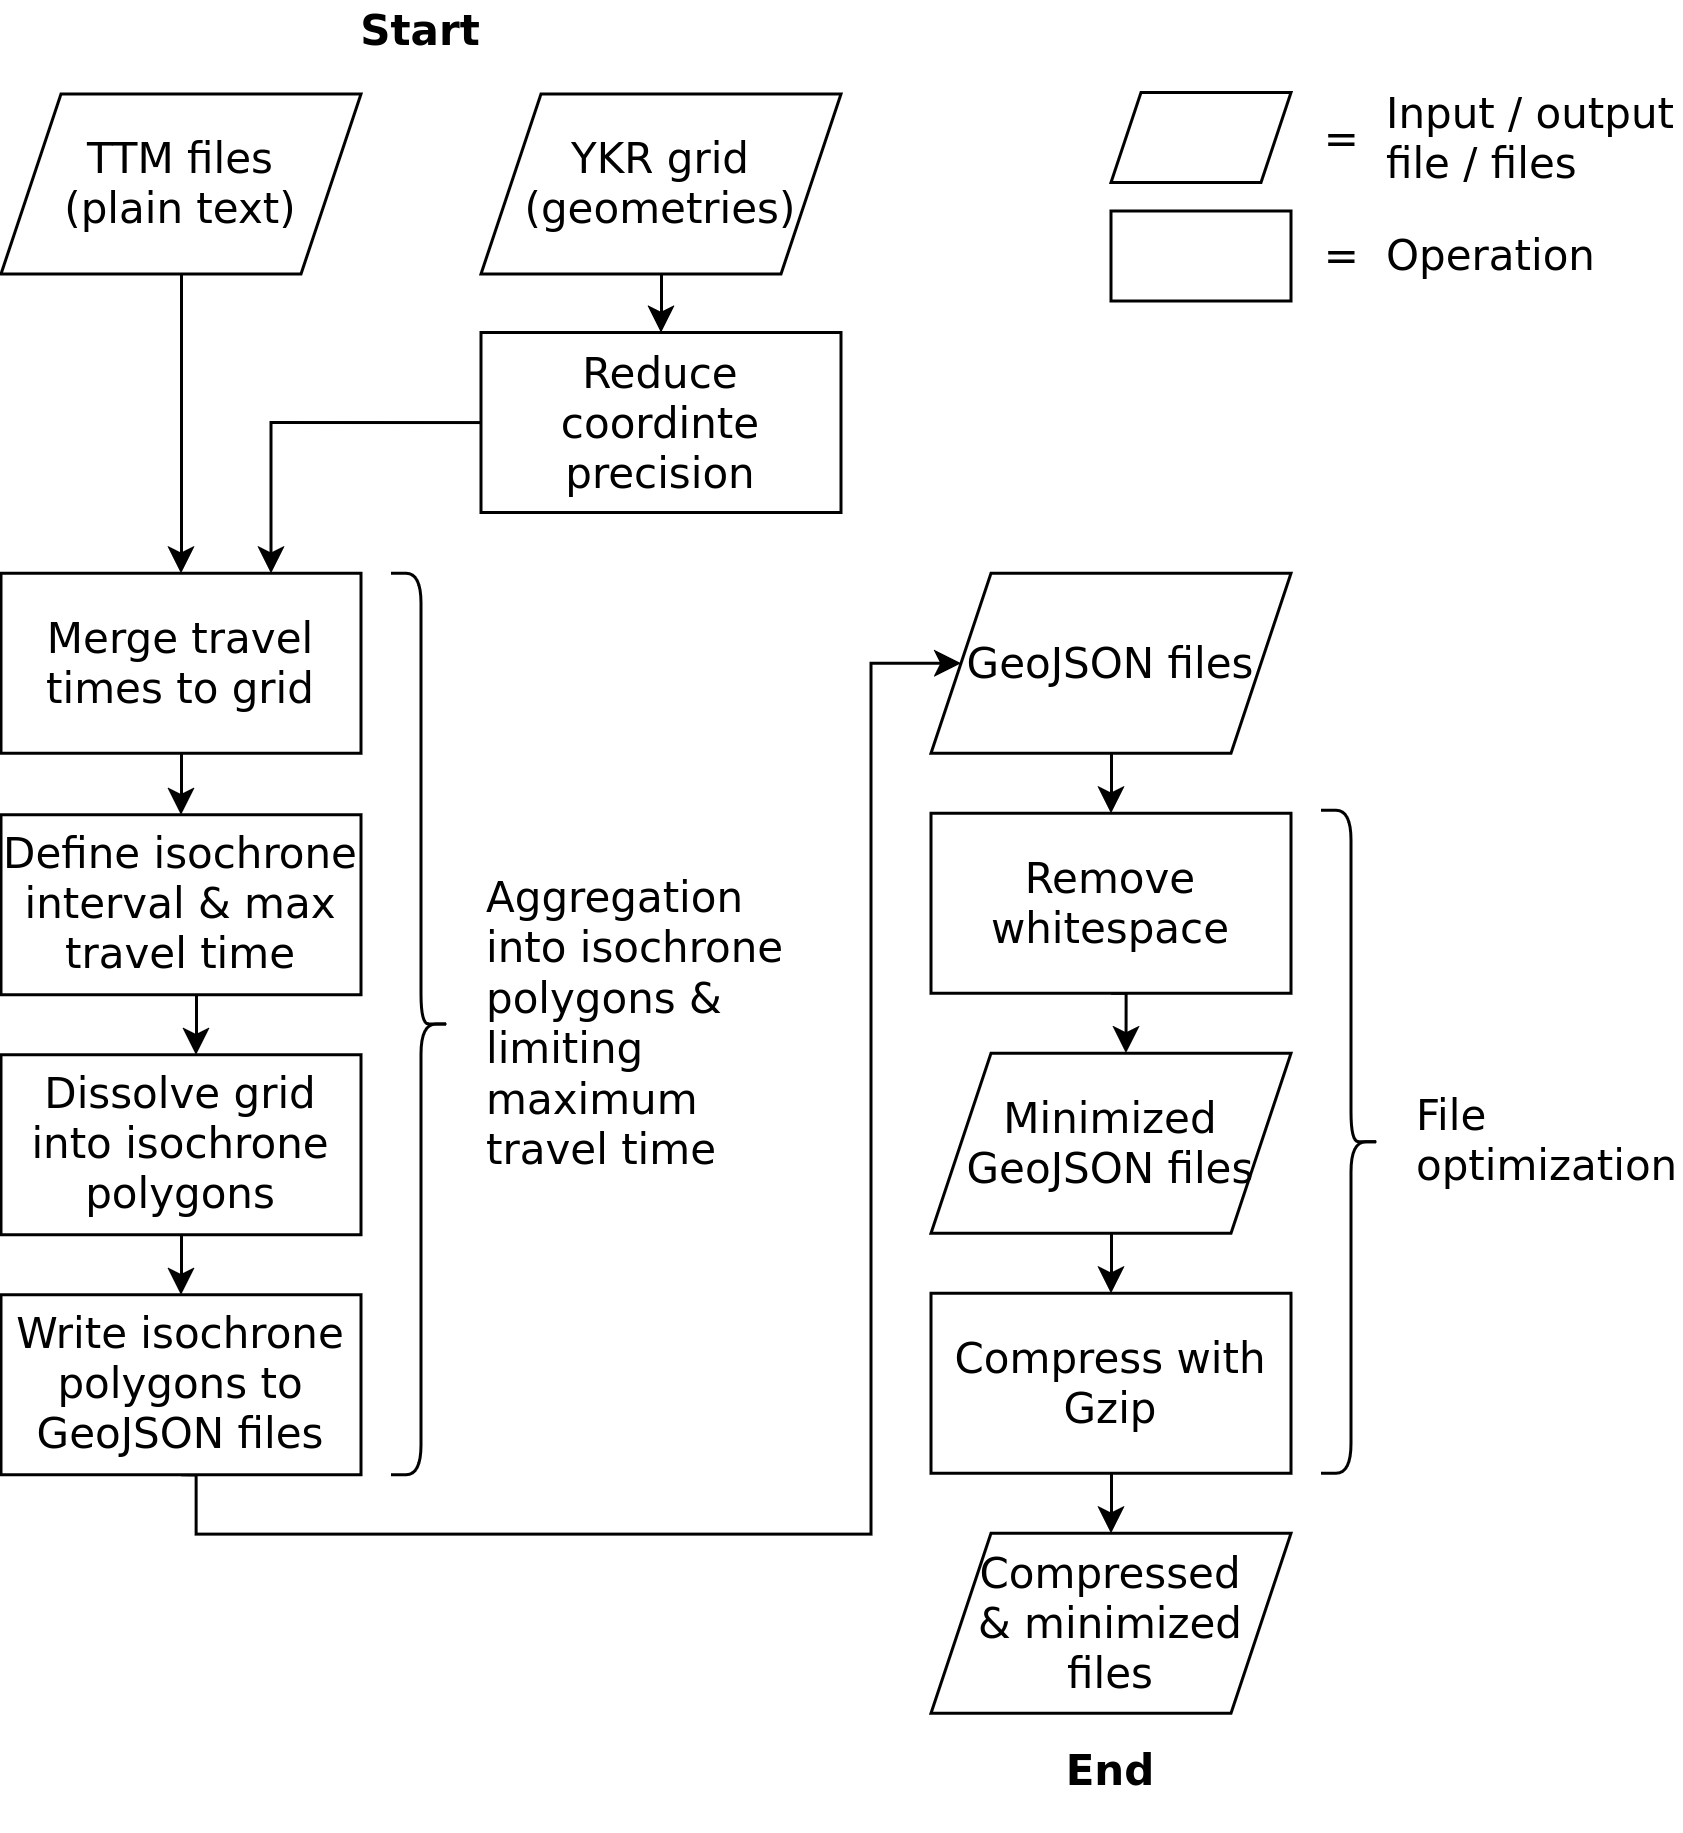
\includegraphics[width=\diagramwidth]{visual/figures/diagrams/preprocessing.png}
	\caption{Preprocessing}
	\label{fig:preprocessing}
\end{figure}

To measure the effects on file sizes,
I calculated the mean combined file size of the all the files needed to represent
all the travel modes for a single cell in the dataset
when a given approach has been applied.
I calculated these values as averages of a random sample as described above.

I assessed the impact the preprocessing approaches have on rendering speed
by using the data with the finished map application.
The details of the map application are in the next section.
This assessment was qualitative,
as it was based on my own perception of responsiveness when using the map.
Quantitative testing of rendering speed would have been preferable,
but it proved to be difficult.
While many tools for profiling the rendering speed of web applications exist,
I did not succeed in two main areas
that would have been necessary for representative results.
I did not manage to limit the timing to strictly the map
component of the interface in such a way that
the test results would be reproducible.
I also did not find a way to automate a set of renders
on a sample of locations.
Averaging the renders of a single location would not suffice
due to the differences of data complexity between locations.
The tools I tried were the Firefox profiler \parencite{firefoxprofiler}
and the React developer tools browser extension \parencite{reactdevtools}
on Firefox and Chromium. % TODO

I carried out the assessment of loss of information in two ways:
Qualitatively for all approaches by observing the processed data on the map,
and, in the case of limiting maximum travel time,
quantitatively by calculating the percentage of the total dataset area
that the processed data covers.
These percentages are, again, averages of a random sample as described above.

Appendix \ref{appendix:repositories} includes a link to the repository
containing the preprocessing pipeline.
The same repository also holds the quantitative tests described above
as an interactive Jupyter Notebook.


\subsubsection{Assessing web mapping libraries and implementing the frontend}

Considering this study,
the map interface is the most crucial component of the application.
It is the frontend that a user interacts with,
providing the \acrshort{ui} capabilities.
The web mapping library plays a key part in implementing the interface,
and in enabling the entire application.
In addition to rendering data correctly and efficiently,
the web mapping library needs to enable user-map interactions to be
captured and propagated to the underlying application.
The underlying application in this case, as mentioned in
section \ref{software requirements},
is a web map application
that, in addition to mapping,
handles various modes of interaction,
\acrshort{http} requests and responses, and data access.
So, an interaction exchange with the map
must be able to alter application state outside the map.
For example,
clicking the map results in the fetching of new data from the backend,
as well as toggling the mode of location selection.

As mentioned in section \ref{sec:web maps},
managing state in web-applications can be complex.
Keeping in mind the requirements specified for this particular application
(section \ref{software requirements}),
as well as the necessity of \acrshort{spa} design,
I considered a general-purpose \acrshort{ui} framework
essential to provide a robust way of controlling the state of the frontend.
Also, in general, using a framework instead of a self-made solution
means less room for error in the implementation,
and better maintainability and extensibility as the amount of code is drastically smaller.
In this study I used React \parencite{react} as the \acrshort{ui} framework
for three reasons:
It is the framework I am most familiar with,
it is the most widely used and documented framework,
and also it is the only framework that
multiple web-mapping libraries have integration capabilities for.

With the above considerations in mind,
I based my assessment of web mapping libraries on three criteria:
\begin{itemize}
	\item Visual quality of the map
	\item Responsiveness of the map
	\item UI integration capabilities (tested only with React)
\end{itemize}

When selecting which web mapping libraries to assess,
I used three properties as a baseline.
The library should be licensed as \presentacr{foss},
It should be actively maintained,
and it should have capabilities to integrate to a general purpose UI framework.
As stated above, the third property meant, in practice, React.
With these considerations I arrived at three web mapping libraries:
Leaflet \parencite{leaflet}, Maplibre \parencite{maplibre} and Deck.gl \parencite{deckgl}.
More precisely, in the case of Maplibre I used the React Map GL wrapper
\parencite{reactmapgl} for integrating maplibre and react, and in the case of Leaflet
I used the React Leaflet wrapper \parencite{reactleaflet} for the same purpose.

To assess these libraries,
I used each of them as the map interface of the frontend. % ref frontend fig here?
To enable such testing in any sensible amount of time,
I took care to implement the frontend in a highly modular way.
The UI component responsible for map rendering and interaction
only required access to the mapped data,
and a way to alter the mapped location.
Aside from these two aspects,
the map component and its internal state was completely encapsulated
from the other components of the frontend application.
This meant that swapping the map library
required no changes to the application outside the map component,
and that as few as possible variables other than the mapping library were changed.

Outside the map component,
the frontend was extremely minimal.
UI-wise, it only included a drop-down menu for selecting travel modes, and a legend.
Functionally, a single service for communicating with the backend was needed,
which I implemented with the Axios \acrshort{http} library \parencite{axios}.
For a visual overview of the map interface see figure \ref{fig:frontend screenshot},
and for the architecture of the frontend see figure \ref{fig:frontend architecture}.

\begin{figure}[H]
	\centering
	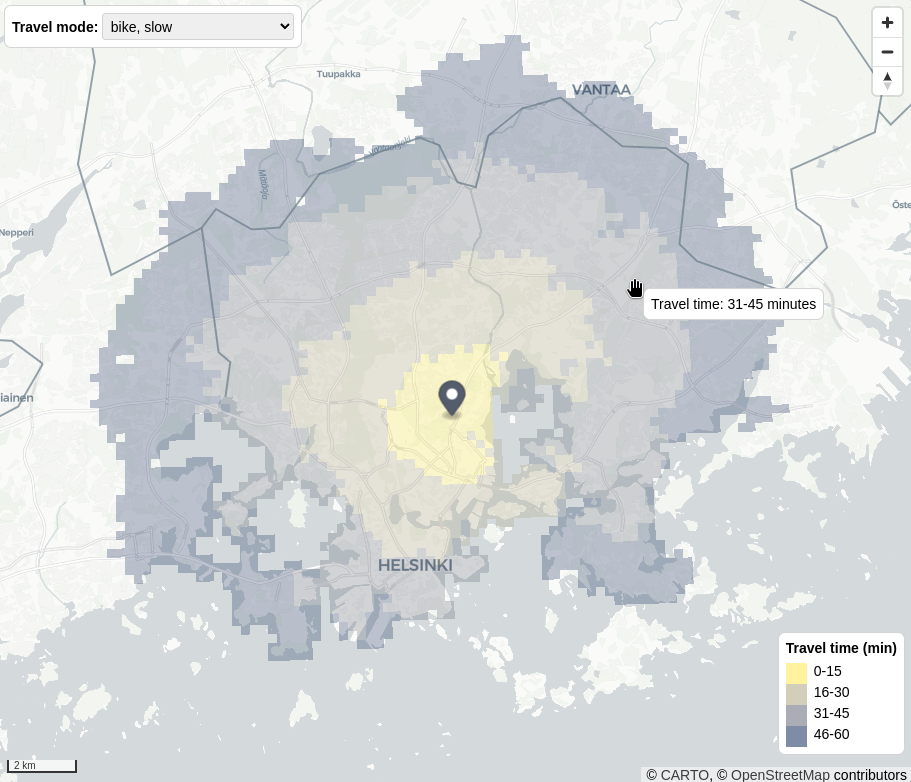
\includegraphics[width=\textwidth]{visual/figures/screenshots/frontend.png}
	\caption{
		The UI of the map application.
		In addition to the map and its control buttons,
		there is a drop-down menu for selecting travel-modes, and a legend.
		Here, the map has been clicked to toggle the mode of interaction
		so that the map does not update with cursor movement.
		Instead, a tooltip with travel time information is displayed under the cursor.
	}
	\label{fig:frontend screenshot}
\end{figure}

\begin{figure}[H]  % TODO location?
	\centering
	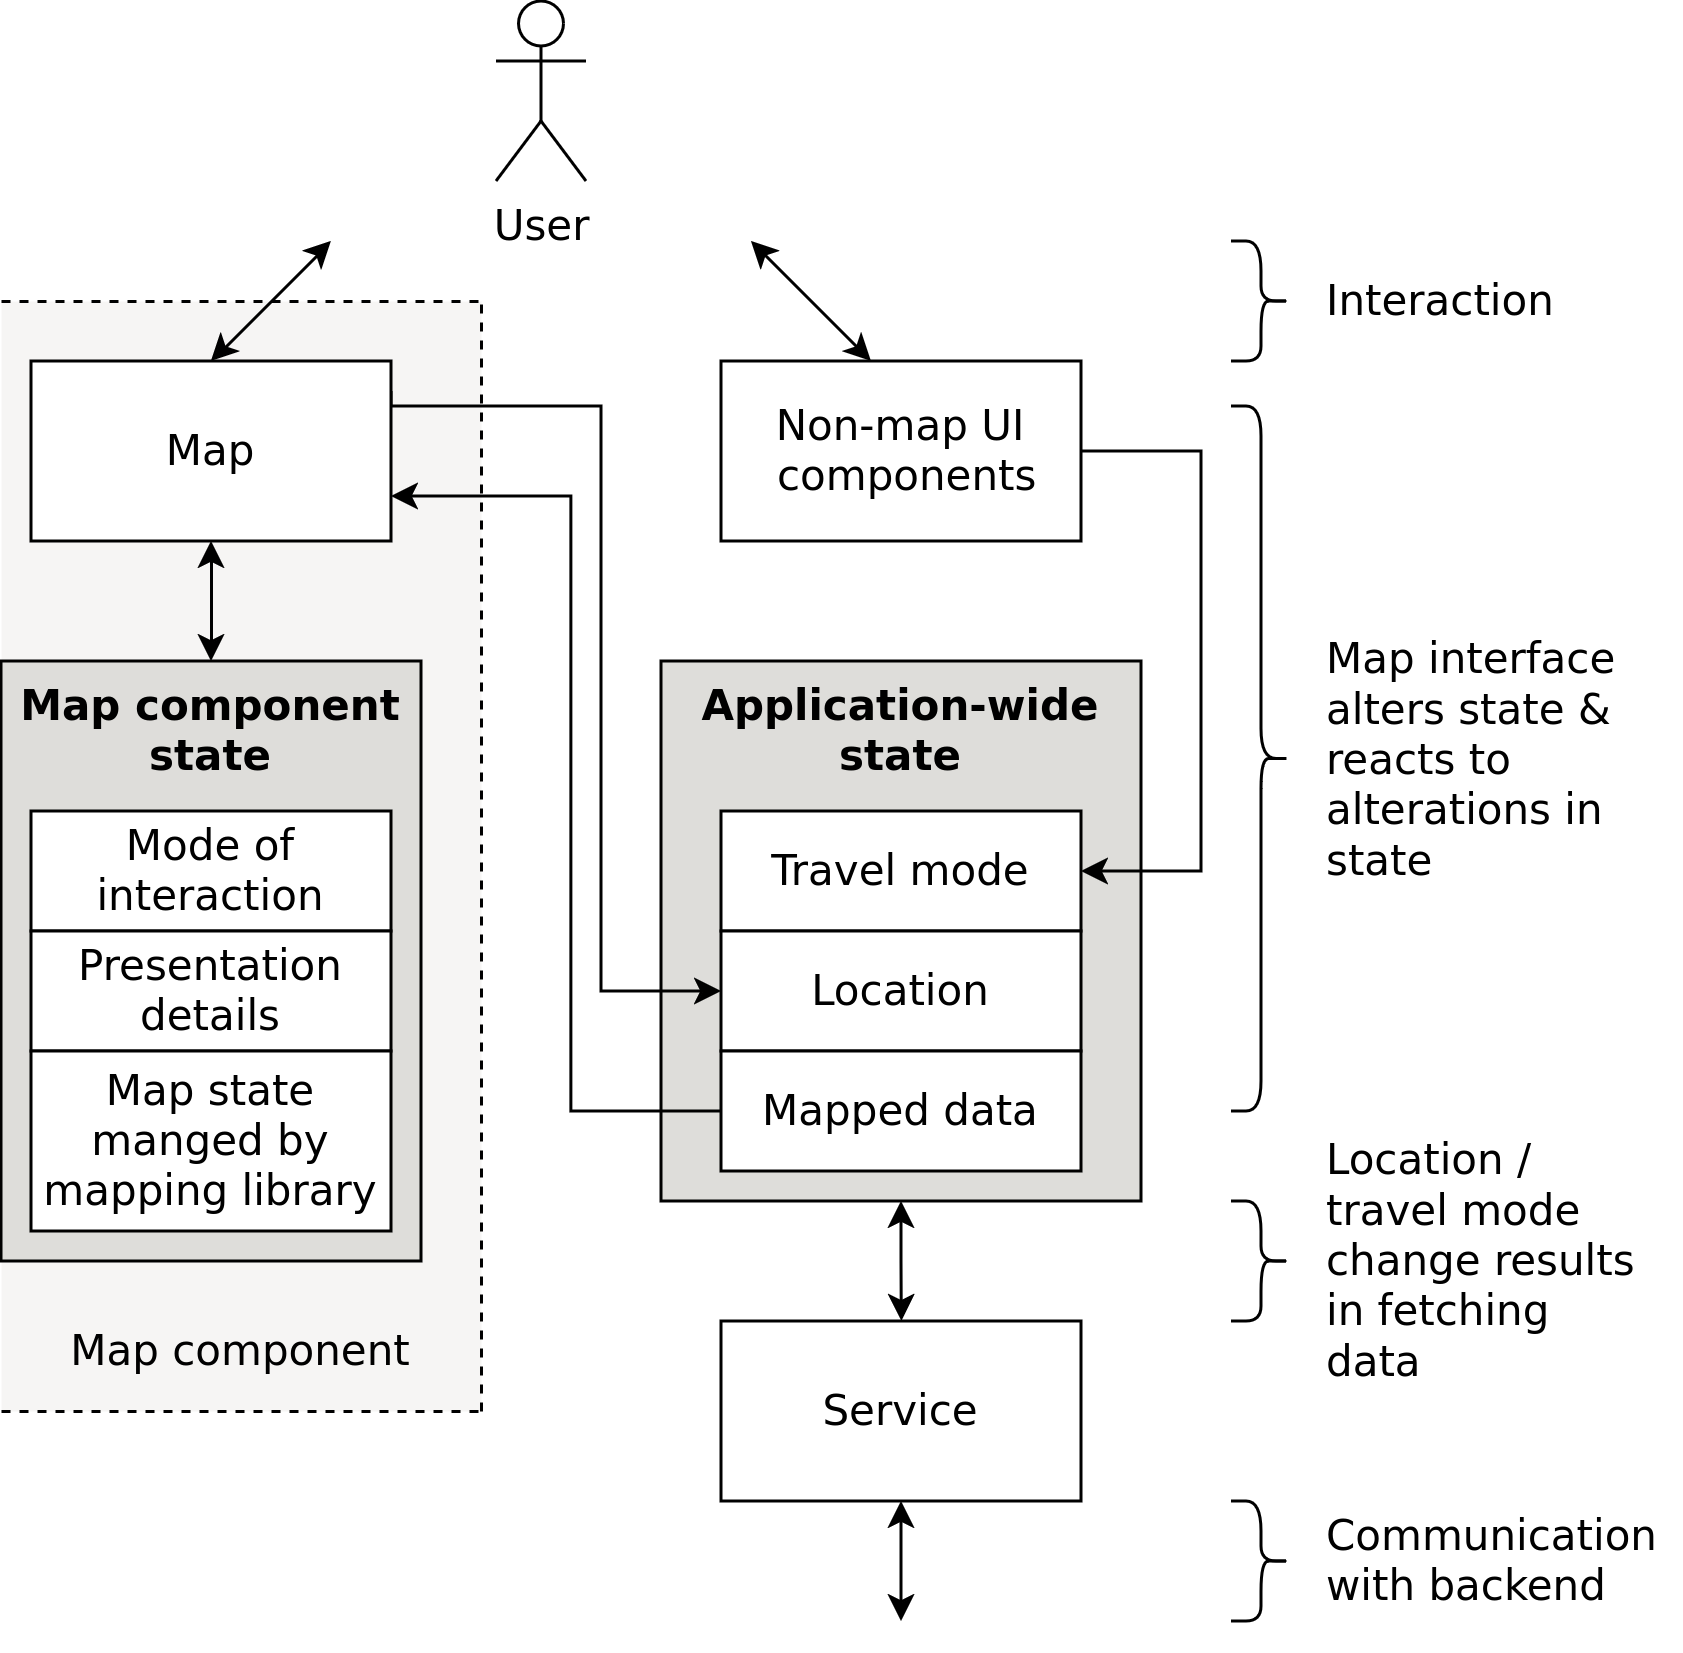
\includegraphics[width=\diagramwidth]{visual/figures/diagrams/frontend.png}
	\caption{
		The frontend architecture.
		The map component is responsible for map rendering and interaction
		as well as all map-specific state.
		All the additional, non-map, UI components are grouped together here,
		as functionally they alter the application state in only one way.
	}
	\label{fig:frontend architecture}
\end{figure}

I assessed the visual quality of the map qualitatively.
For the reasons I stated in section \ref{sec:preprocessing},
I had to resort to qualitative assessment
for assessing the rendering performance as well.
For assessing integration with react I utilized online documentation of potential solutions,
as well as my development experience in implementing the frontend.

A link to the repository containing the code
and further technical details of the frontend
can be found in appendix \ref{appendix:repositories}.

% % TODO copypasta
% Translucent Overlay (OV) is the best technique over-
% all, which makes it a good choice when only one comparison
% technique should be provided to user \parencite{lob2015}.


\subsubsection{Application deployment and other technical infrastructure}

\begin{itemize}
	\item Backend: Minimal HTTP sever serving pre-compressed geojson files directly from filesystem
	\item Scalable Kubernetes / OpenShift deployments → Reproducibility at the level of the entire application
	\item Containerization → Reproducibility at the level of the components of the application
	\item Modularity of the design
	\item the list goes on, I'll have to consider what matters and what doesn't.
\end{itemize}

\begin{figure}[H]
	\centering
	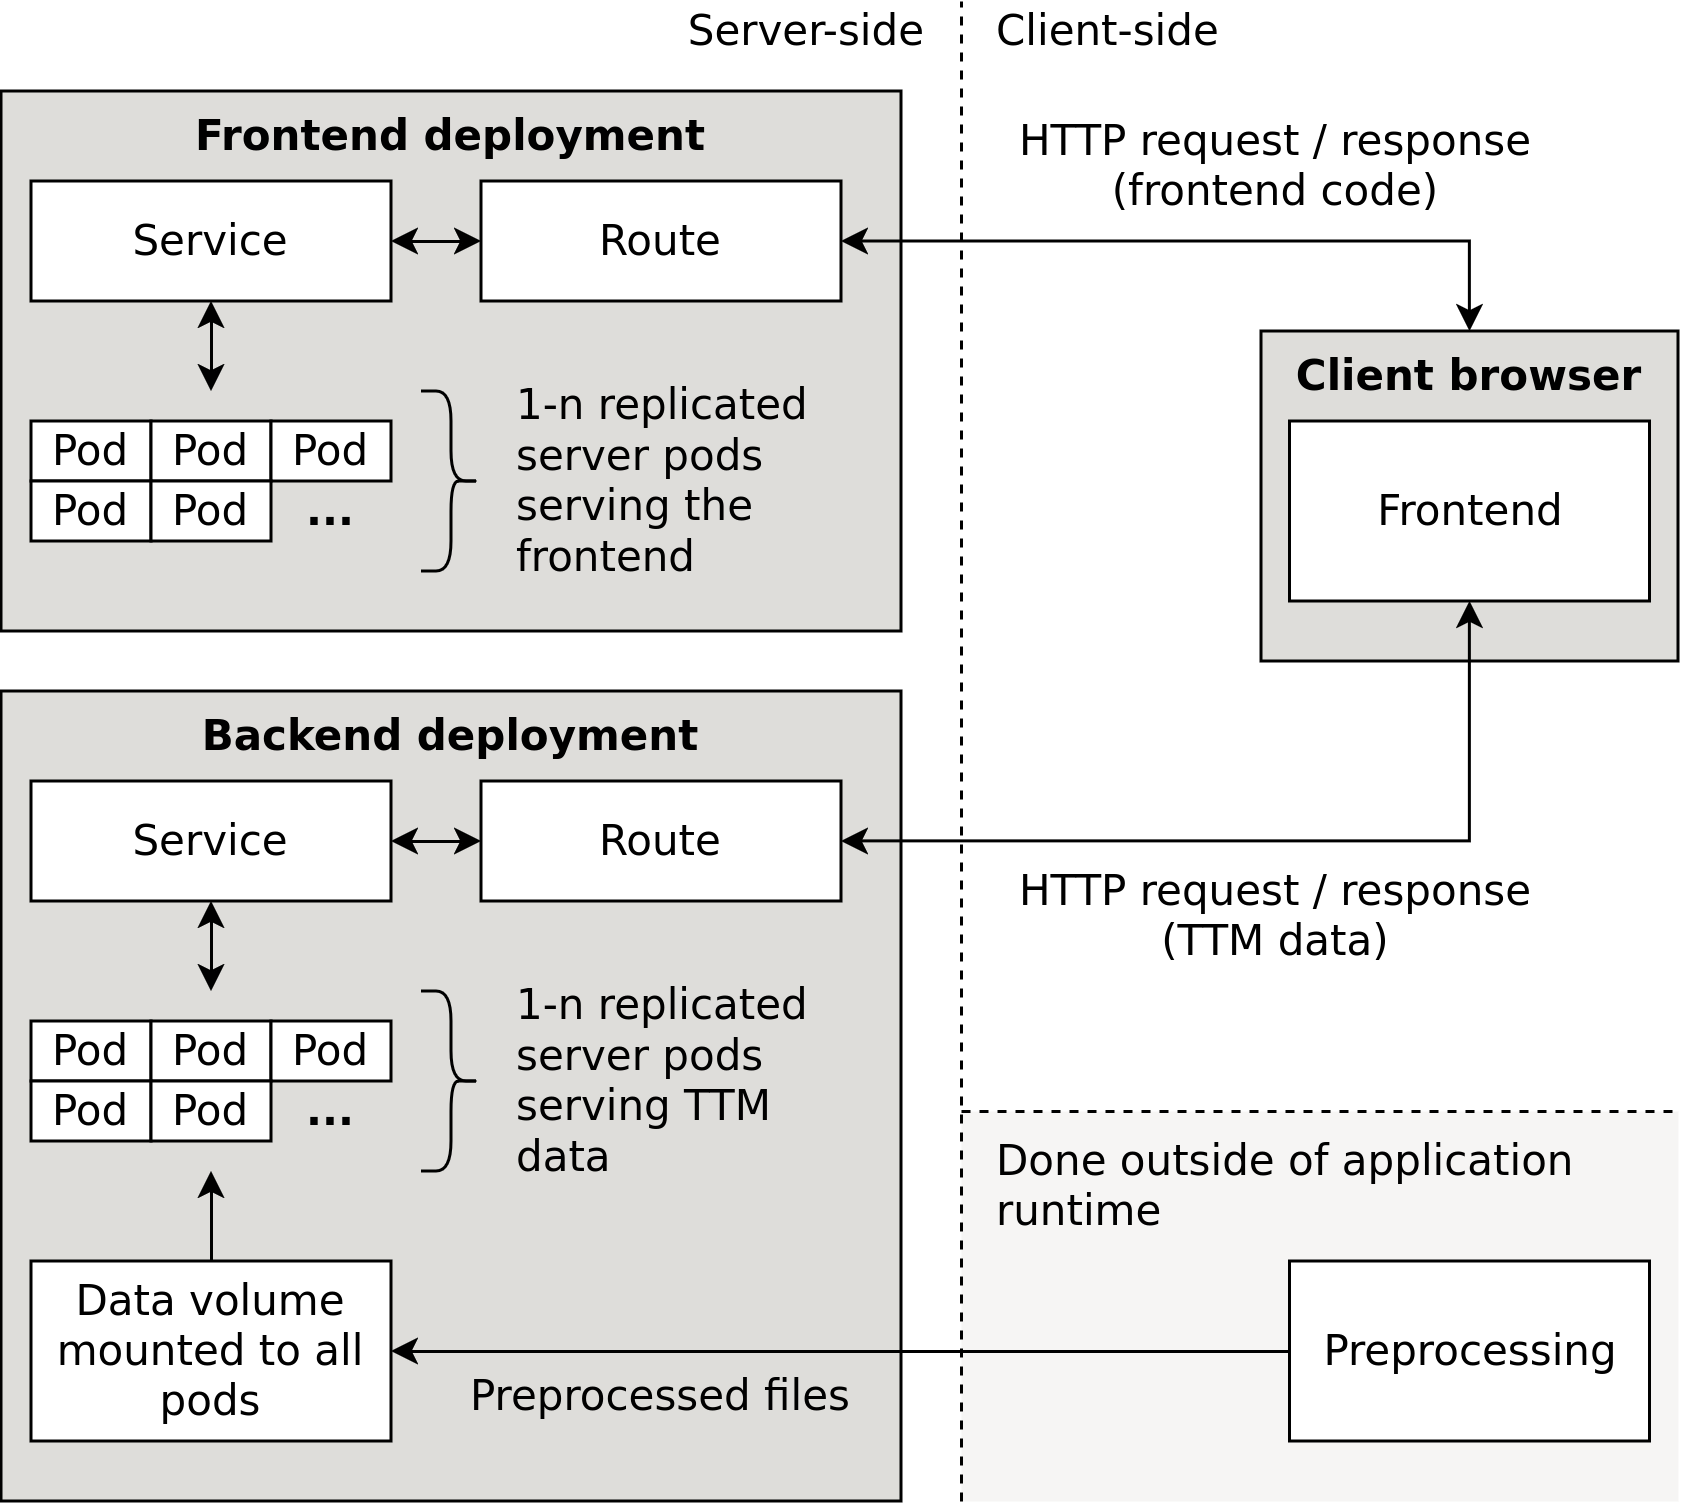
\includegraphics[width=\diagramwidth]{visual/figures/diagrams/architecture.png}
	\caption{Architecture}
	\label{fig:architechture}
\end{figure}

In short, containerization refers to a set of technologies
that enables packaging software and all its necessary components
into self-contained \textit{container images} that can be run as is,
regardless of the specifics of the underlying system.

SIDENOTE: I'll add figures of the components (at least the map application) here as suggested by Pyry.


% The need for serving (backend)
% - why data must be decoupled
% && the requirements serving must satisfy

% Different approaches

% Why nginx + static files?

% Describe how it was done

\subsection{Survey}

\subsubsection{Questionnaire design and structure}

The questionnaire is structured to:
\begin{itemize}
	\item Prompt the participant to use the map for different tasks
	\item Ask questions about the participant's experience
	on using the map for completing the tasks
\end{itemize}

Reasoning about the design: online questionnaire, tasks composed of prompts and questions.
Descriptions of what the purpose of each task was.

\subsubsection{Questionnaire distribution and participants}
How the survey was distributed,
Description of the sample.

(Response plots in appendices)

\section{Results}
Selected preprocessing / serving / mapping approaches
Survey results
The map application

\subsection{Data preprocessing}

\subsection{Application design}

See \ref{tab:map library comparison} for comparison of mapping libraries.


% TODO Describe why these libraries were selected
% Baseline: FOSS, Actively maintained

\begin{table}[h]
	\centering
	\begin{tabular}{ L{0.1\textwidth} | L{0.25\textwidth} | L{0.25\textwidth} | L{0.25\textwidth} }
		\raggedright
		Library
		& Quality of visualisation
		& Rendering performance
		& Integration with React
		\\ 
		\hline
		Deck.gl
		& Inconsistent rendering of complex polygons, vector tiles supported
		& GPU accelerated (WebGL), most performant of the tested libraries
		& Designed from ground up to work with React
		\\
		\hline
		Leaflet
		& Correct rendering of shapes, Vector tiles possible through plugins
		& No GPU acceleration, least performant of the tested libraries
		& Integration possible with a 3rd party wrapper
		\\
		\hline
		Maplibre
		& Mostly correct rendering of polygons with very rare inconsistancies, vector tiles supported
		& GPU accelerated (WebGL), slightly less performant than Deck.gl
		& Integration possible with a 3rd party wrapper
		\\
		\hline
	\end{tabular}
	\caption{Comparison of mapping libararies}
	\label{tab:map library comparison}
\end{table}

% \begin{table}[h]
% 	\centering
% 	\begin{tabularx}{\textwidth} { 
% 		| >{\raggedright\arraybackslash}X 
% 		| >{\raggedright\arraybackslash}X 
% 		| >{\raggedright\arraybackslash}X 
% 		| >{\raggedright\arraybackslash}X 
% 		| >{\raggedright\arraybackslash}X
% 	}
% 	\hline
% 	asdf & sf & item 11 & item 12 & item 13 \\
% 	\hline
% 	item 21  & item 22  & item 23  \\
% 	\hline
% 	\end{tabularx}
% 	\caption{Comparison of mapping libararies}
% 	\label{tab:map library comparison}
% \end{table}

\subsection{Map usage}

See \ref{fig:Questions 1 and 2} for answers to questions 1 \ref{fig:Question 1} and 2 \ref{fig:Question 2}.

\begin{figure}[H]
	\centering
	\begin{subfigure}[b]{0.5\textwidth}
		\centering
		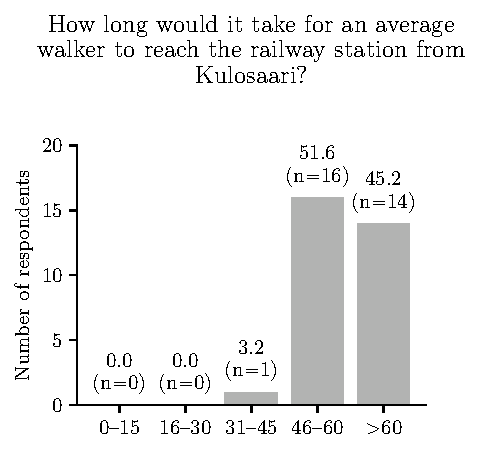
\includegraphics[width=\textwidth]{images/questionnaire/0.pdf}
		\caption{Question 1}
		\label{fig:Question 1}
	\end{subfigure}%
	\hfill
	\begin{subfigure}[b]{0.5\textwidth}
		\centering
		\includegraphics[width=\textwidth]{images/questionnaire/1.pdf}
		\caption{Question 2}
		\label{fig:Question 2}
	\end{subfigure}%
	\caption{Questions 1 and 2}
	\label{fig:Questions 1 and 2}
\end{figure}

\begin{figure}[H]
	\centering
	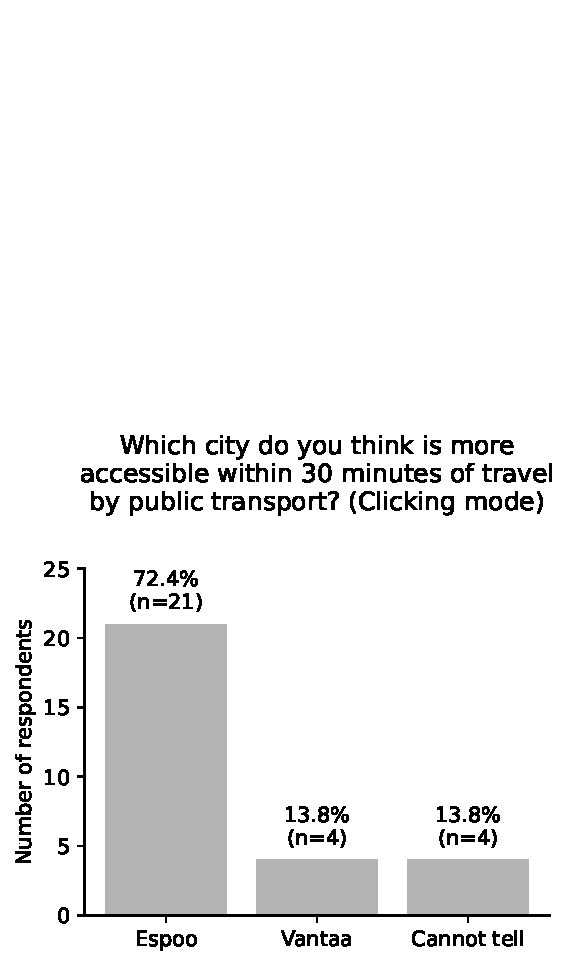
\includegraphics[width=0.5\textwidth]{images/questionnaire/2.pdf}
	\caption{Question 3}
	\label{fig:Question 3}
\end{figure}

\begin{figure}[H]
	\centering
	\begin{subfigure}[b]{0.5\textwidth}
		\centering
		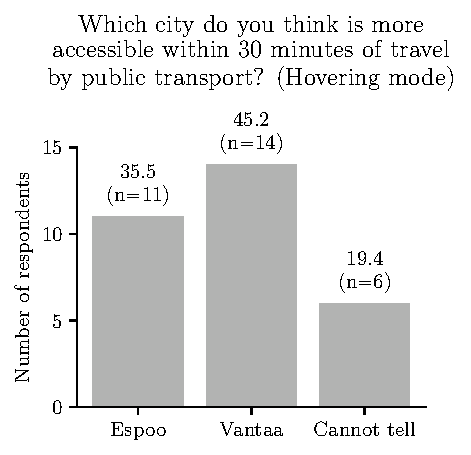
\includegraphics[width=\textwidth]{images/questionnaire/3.pdf}
		\caption{Question 4}
		\label{fig:Question 4}
	\end{subfigure}%
	\hfill
	\begin{subfigure}[b]{0.5\textwidth}
		\centering
		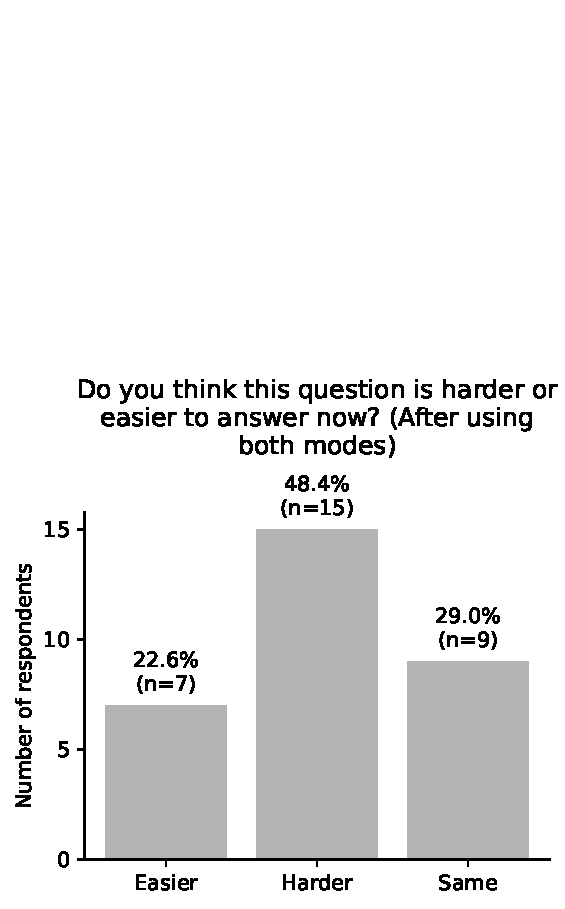
\includegraphics[width=\textwidth]{images/questionnaire/4.pdf}
		\caption{Question 5}
		\label{fig:Question 5}
	\end{subfigure}%
	\caption{Questions 4 and 5}
	\label{fig:Questions 4 and 5}
\end{figure}

% \begin{figure}[H]
% 	\centering
% 	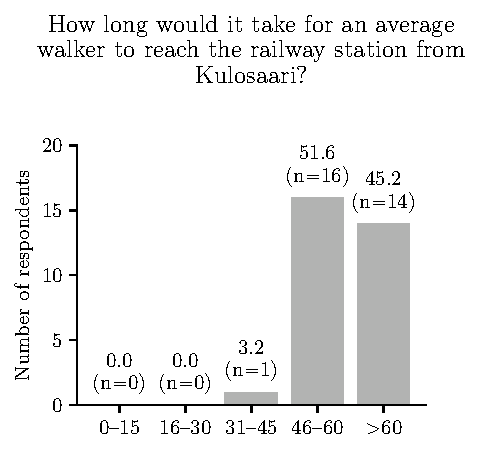
\includegraphics[width=0.75\textwidth]{images/questionnaire/0.pdf}
% 	\caption{Question}
% 	\label{fig:architechture}
% \end{figure}

% \begin{figure}[H]
% 	\centering
% 	\includegraphics[width=0.75\textwidth]{images/questionnaire/1.pdf}
% 	\caption{Question}
% 	\label{fig:architechture}
% \end{figure}

% \begin{figure}[H]
% 	\centering
% 	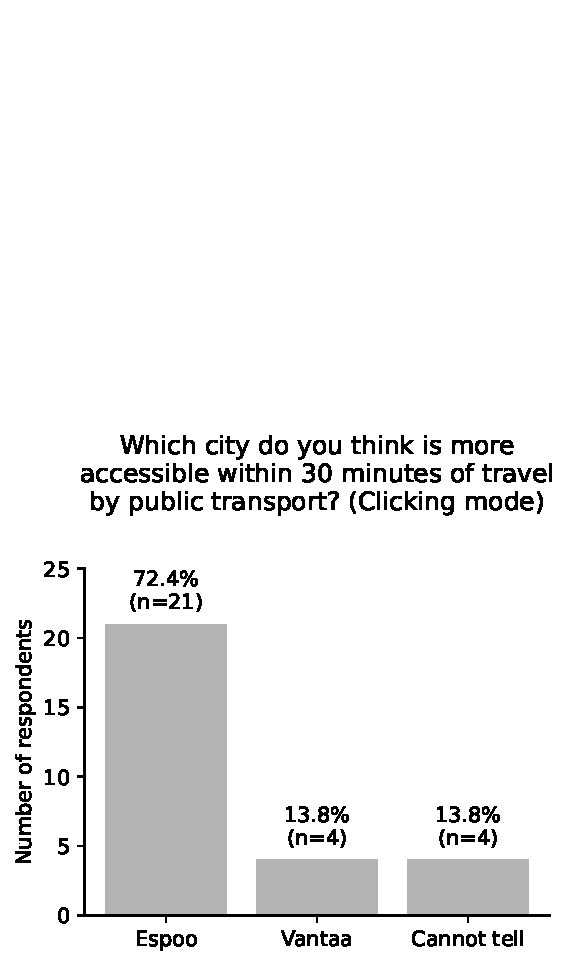
\includegraphics[width=0.75\textwidth]{images/questionnaire/2.pdf}
% 	\caption{Question}
% 	\label{fig:architechture}
% \end{figure}

% \begin{figure}[H]
% 	\centering
% 	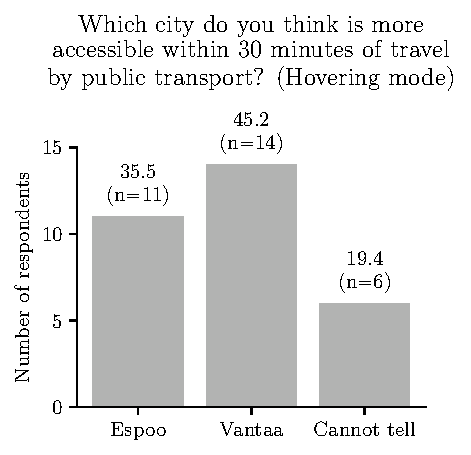
\includegraphics[width=0.75\textwidth]{images/questionnaire/3.pdf}
% 	\caption{Question}
% 	\label{fig:architechture}
% \end{figure}

% \begin{figure}[H]
% 	\centering
% 	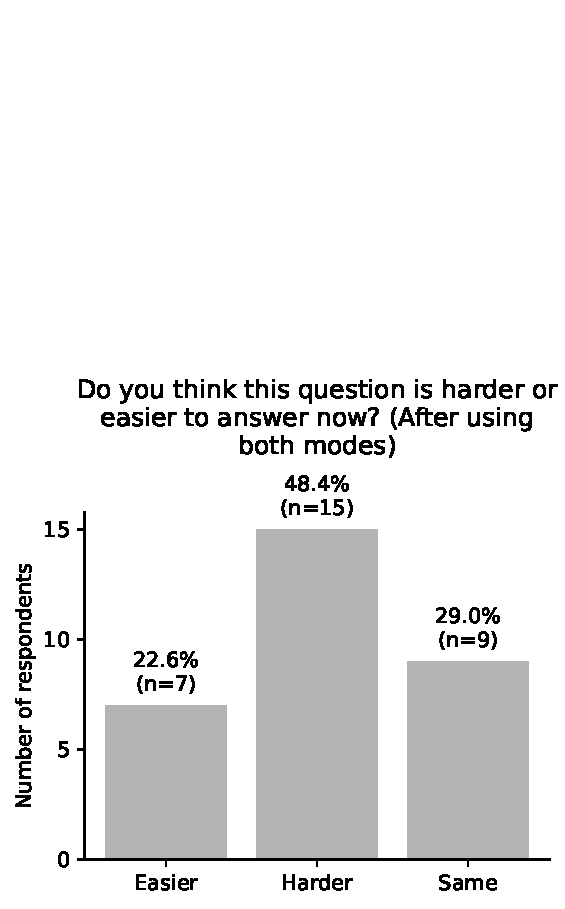
\includegraphics[width=0.75\textwidth]{images/questionnaire/4.pdf}
% 	\caption{Question}
% 	\label{fig:architechture}
% \end{figure}

% \begin{figure}[H]
% 	\centering
% 	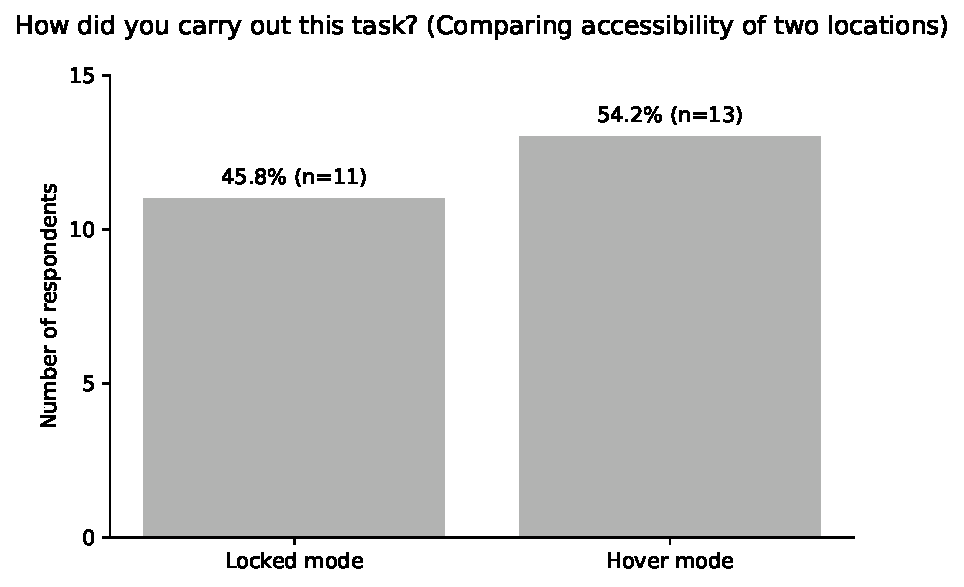
\includegraphics[width=0.75\textwidth]{images/questionnaire/5.pdf}
% 	\caption{Question}
% 	\label{fig:architechture}
% \end{figure}

% \begin{figure}[H]
% 	\centering
% 	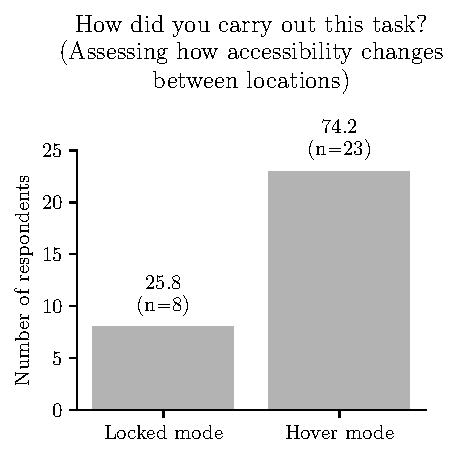
\includegraphics[width=0.75\textwidth]{images/questionnaire/6.pdf}
% 	\caption{Question}
% 	\label{fig:architechture}
% \end{figure}

% \begin{figure}[H]
% 	\centering
% 	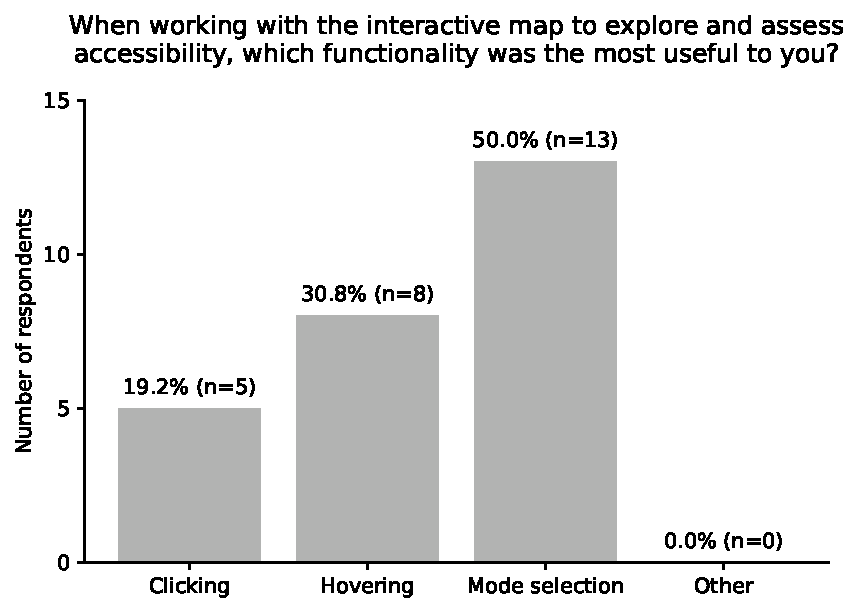
\includegraphics[width=0.75\textwidth]{images/questionnaire/7.pdf}
% 	\caption{Question}
% 	\label{fig:architechture}
% \end{figure}

% \begin{figure}[H]
% 	\centering
% 	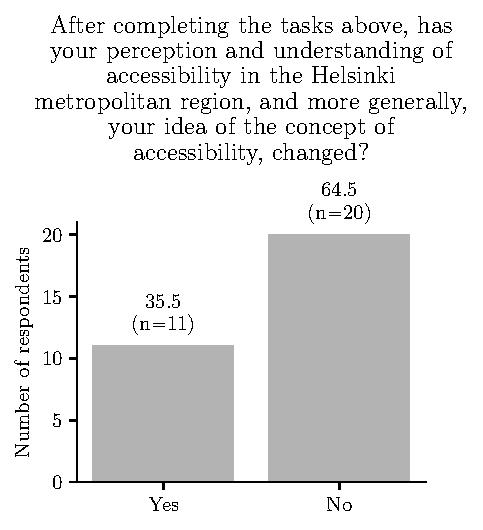
\includegraphics[width=0.75\textwidth]{images/questionnaire/8.pdf}
% 	\caption{Question}
% 	\label{fig:architechture}
% \end{figure}

% \begin{figure}[H]
% 	\centering
% 	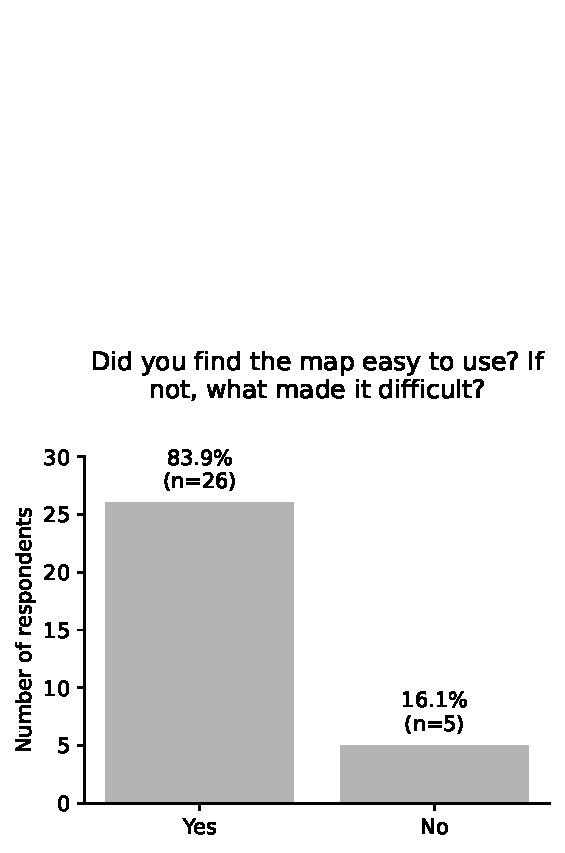
\includegraphics[width=0.75\textwidth]{images/questionnaire/9.pdf}
% 	\caption{Question}
% 	\label{fig:architechture}
% \end{figure}

% \begin{figure}[H]
% 	\centering
% 	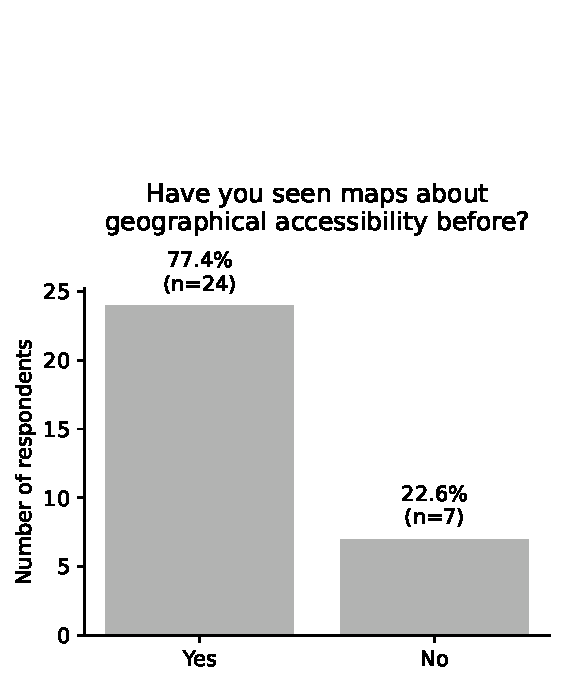
\includegraphics[width=0.75\textwidth]{images/questionnaire/10.pdf}
% 	\caption{Question}
% 	\label{fig:architechture}
% \end{figure}

% \begin{figure}[H]
% 	\centering
% 	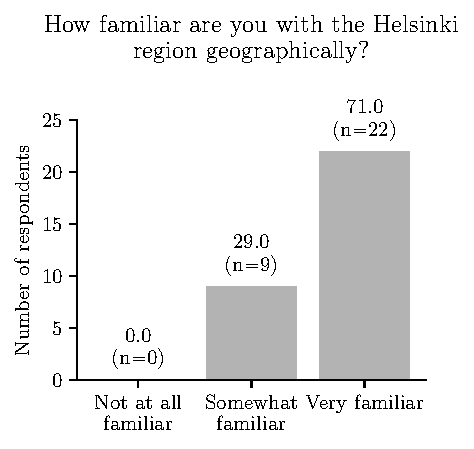
\includegraphics[width=0.75\textwidth]{images/questionnaire/11.pdf}
% 	\caption{Question}
% 	\label{fig:architechture}
% \end{figure}

% \begin{figure}[H]
% 	\centering
% 	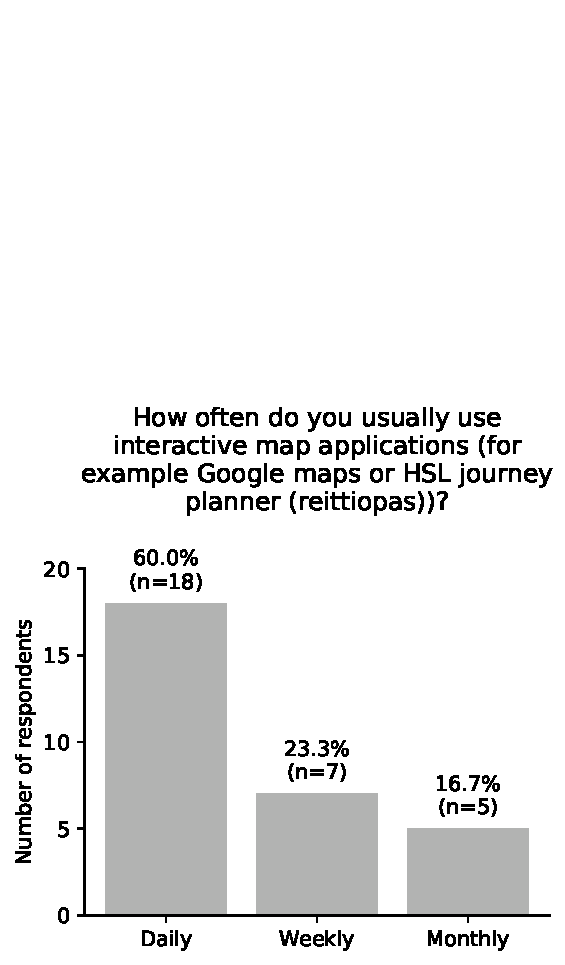
\includegraphics[width=0.75\textwidth]{images/questionnaire/12.pdf}
% 	\caption{Question}
% 	\label{fig:architechture}
% \end{figure}

% \begin{figure}[H]
% 	\centering
% 	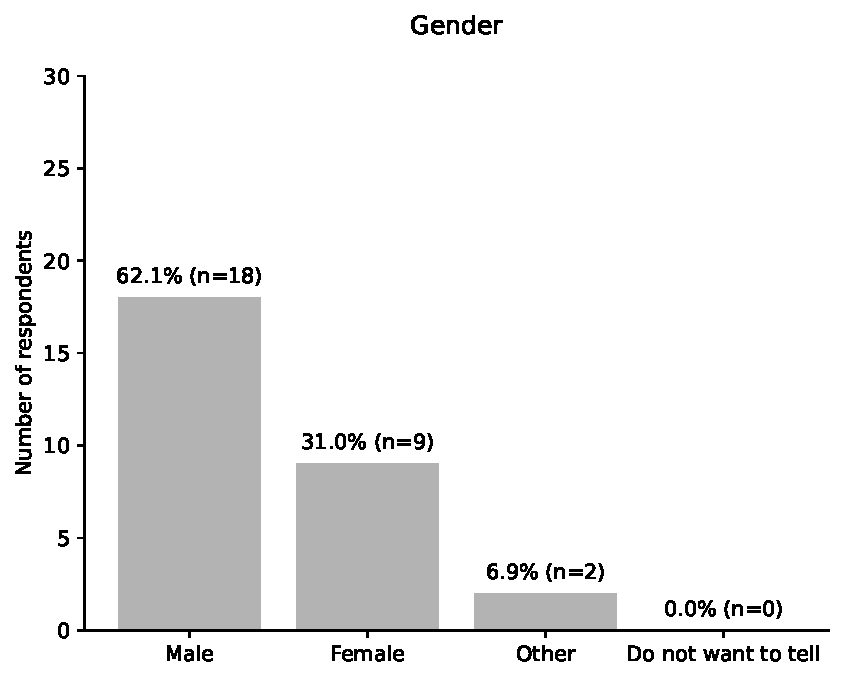
\includegraphics[width=0.75\textwidth]{images/questionnaire/13.pdf}
% 	\caption{Question}
% 	\label{fig:architechture}
% \end{figure}

% \begin{figure}[H]
% 	\centering
% 	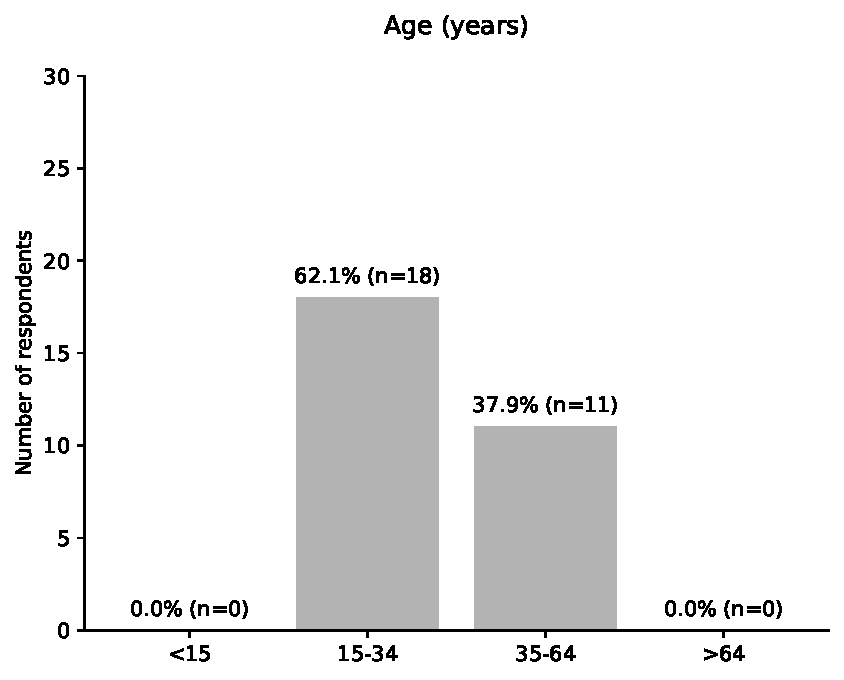
\includegraphics[width=0.75\textwidth]{images/questionnaire/14.pdf}
% 	\caption{Question}
% 	\label{fig:architechture}
% \end{figure}

\section{Discussion}

Some ideas for discussion:
\begin{itemize}
	\item Pros and cons of real-time interaction:
	Implementing something like the hover mode could be worth it in the sense
	that it provides a genuinely different way to explore massive data.
	Depending on the data being visualized,
	the loss of detail to enable such a presentation could be immense,
	potentially leading to a shallow presentation with little insight to offer.
	\item Too much data / too precise data:
	Scaling this type of approach to even more data could be difficult. Can data be too detailed?
	\item Tradeoffs in the map:
	now priority is on instant interaction instead of detailed maps.
	What would the map, and by extension the whole study, look like with different priorities?
	\item Reproducibility and open science:
	The \acrshort{ttm} is not only an open dataset but also an open method.
	This work continues on that track,
	as every component is completely open-source \& openly available.
	\item Amount of work \& the need for cooperation:
	Mapmaking is a very small fraction of all the work that goes into implementing cartographic interaction,
	yet all the other work must be done, or the map will not exist.
	Cooperation with developers, map users and cartographers is key.
\end{itemize}

% My results showed that...
\subsection{Real time cartographic interaction and its tradeoffs}

% The map presentation and survey results from cartography perspective
Implementing something like the hover mode could be worth it in the sense
that it provides a genuinely different way to explore massive data.
Depending on the data being visualized,
the loss of detail to enable such a presentation could be immense,
potentially leading to a shallow presentation with little insight to offer.

Tradeoffs in the map:
now priority is on instant interaction instead of detailed maps.


\subsection{Technical considerations in producing interactive maps}

Many of the tradeoffs above are not inherent to cartographic interaction,
rather they are technical limitations.

% The map presentation and survey results from technical perspective
Too much data / too precise data:
Scaling this type of approach to even more data could be difficult.
Can data be too detailed?

Amount of work and the need for cooperation:
Mapmaking is a very small fraction of all the work
that goes into implementing cartographic interaction,
yet all the other work must be done,
or the map will not exist.
Cooperation with developers, map users and cartographers is key.

Generalization of results is difficult if not impossible

Difficulty in assessing options: Testing the technology or the implementation.

% Accessibility? A whole different technology stack and an immense amount of work

\subsection{Open source and open science -- measurements, modelling, data and mapping}

% TTM overview: measurements, modelling, dataset
Not only a dataset, the \acrshort{ttm} is an extensive showcase of open science.

% Not complete without representation
In many cases, open access to data does not by itself enable
the exploration or understanding of said data \parencite{obr2016}.
It could be argued that the \acrshort{ttm} is a prime example of this.
In its raw, unprocessed, form,
the dataset constitutes gigabytes of data spread over thousands of plain text files
that need to be further combined with an external statistical grid to enable
geographical representation of the data.
Merely comprehending the structure of the dataset requires expertise,
proving to be anything but obvious even to university students specializing in the field
-- the author included.
Even though the latest iteration of the dataset \parencite{fin2023}
includes an easier-to-map data format with geometries included,
actually mapping the \acrshort{ttm} would still require
desktop \acrshort{gis} software or a programming language installation,
coupled with the know-how of using either option.
An open representation for open data

% The representation from the angle of access to understanding data, reproducibility and open science
This work continues on that track,
as every component is completely open-source \& openly available.


\subsection{What was not mapped}

A lot. By this I mean that the options in
conceptualizing, implementing and studying an interactive map presentation are innumerable.

What would the map, and by extension the whole study, look like with different priorities?

Further research:


\section{Conclusions}

\section{Conclusions}

As web map applications grow both in complexity and in demands for performance and usability,
keeping up with the progress of web technologies is essential.

Map functionalities cannot be afterthoughts.

Cartographic interaction as enabled by digital map interfaces

\section*{Acknowledgements}
\addcontentsline{toc}{section}{Acknowledgements}

Thank you Tuuli, Chris and Pyry for all the help and guidance during this process.
Additionally,
I thank Tuuli for providing me with literature and
helping with distributing the questionnaire,
Chris for setting up the necessary CSC projects,
and the Digital Geography Lab for providing me an opportunity to demonstrate and test the
interactive map in a workshop setting.


% Bibliography in toc
\clearpage
\addcontentsline{toc}{section}{References}

\printbibliography

% \clearpage
% \pagestyle{empty}

\begin{appendices}
\makeatletter
\renewcommand{\thesubsection}{\@arabic\c@subsection}  % label with numbers instead of letters
\makeatother

\subsection{Questionnaire}

A static print of the online questionnaire used in the study is found below.
Minor aesthetic differences are present due to conversion from a web-page,
but all content is identical.

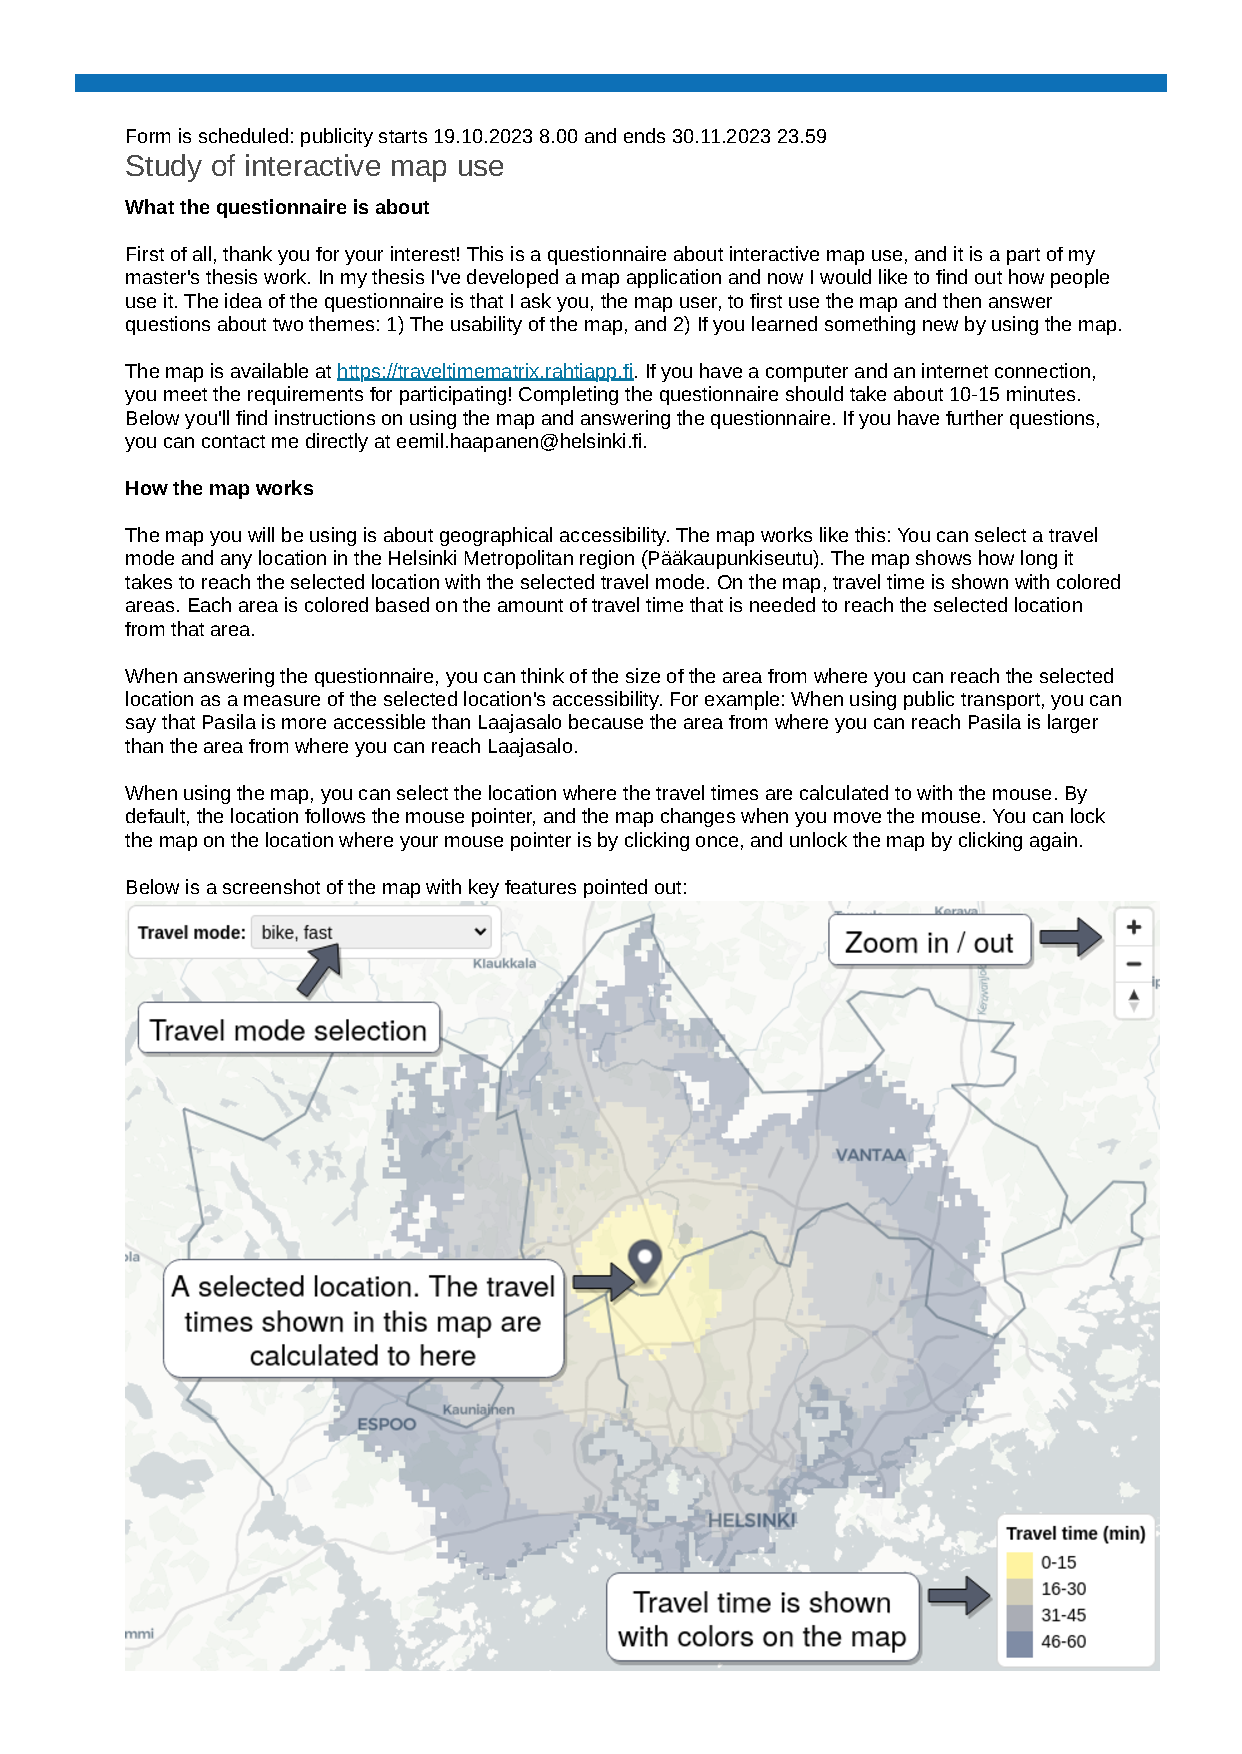
\includepdf[pages={1-},scale=1]{external_pdf/questionnaire.pdf}

\subsection{Questionnaire responses}

Responses to the questionnaire are presented here.
They are divided into the same task groupings that were used in the questionnaire.

\begin{figure}[H]
	% \centering
	\begin{subfigure}[b]{0.5\textwidth}
	% 	\centering
		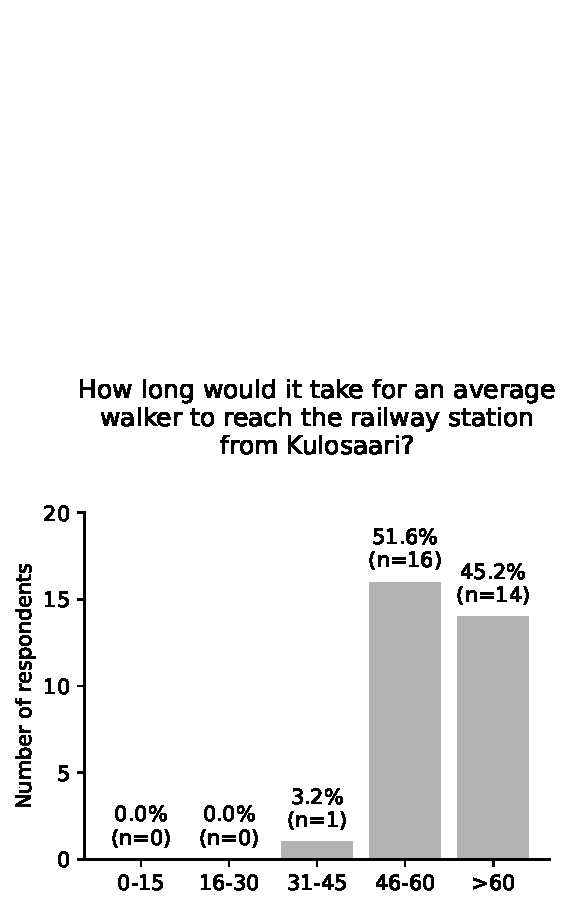
\includegraphics[width=\textwidth]{visual/figures/survey/0.pdf}
	\end{subfigure}%
	\hfill
	\begin{subfigure}[b]{0.5\textwidth}
	% 	\centering
		\includegraphics[width=\textwidth]{visual/figures/survey/1.pdf}
	\end{subfigure}%
	% \caption{Responses to task 1}
	% \label{fig:task 1}
	\newline
	Responses to task 1
\end{figure}

\begin{figure}[H]
	% \centering
	\includegraphics[width=0.5\textwidth]{visual/figures/survey/2.pdf}
	% \caption{Responses to task 2}
	% \label{fig:task 2}
	\newline
	Responses to task 2
\end{figure}

\begin{figure}[H]
	% \centering
	\begin{subfigure}[b]{0.5\textwidth}
	% 	\centering
		\includegraphics[width=\textwidth]{visual/figures/survey/3.pdf}
	\end{subfigure}%
	\hfill
	\begin{subfigure}[b]{0.5\textwidth}
	% 	\centering
		\includegraphics[width=\textwidth]{visual/figures/survey/4.pdf}
	\end{subfigure}%
	% \caption{Responses to task 3}
	% \label{fig:task 3}
	\newline
	Responses to task 3
\end{figure}

\begin{figure}[H]
	% \centering
	\begin{subfigure}[b]{0.5\textwidth}
	% 	\centering
		\includegraphics[width=\textwidth]{visual/figures/survey/5.pdf}
	% 	\caption{Responses to task 4}
	% 	\label{fig:task 4}
	\end{subfigure}%
	\begin{subfigure}[b]{0.5\textwidth}
	% 	\centering
		\includegraphics[width=\textwidth]{visual/figures/survey/6.pdf}
	% 	\caption{Responses to task 5}
	% 	\label{fig:task 5}
	\end{subfigure}
	\newline
	Responses to task 4
\end{figure}

\begin{figure}[H]
	% \centering
	\begin{subfigure}[b]{0.5\textwidth}
	% 	\centering
		\includegraphics[width=\textwidth]{visual/figures/survey/7.pdf}
	\end{subfigure}%
	\hfill
	\begin{subfigure}[b]{0.5\textwidth}
	% 	\centering
		\includegraphics[width=\textwidth]{visual/figures/survey/8.pdf}
	\end{subfigure}%
	\newline
	\begin{subfigure}[b]{0.5\textwidth}
	% 	\centering
		\includegraphics[width=\textwidth]{visual/figures/survey/9.pdf}
	\end{subfigure}%
	% \caption{Responses to general questions}
	% \label{fig:general questions}
	\newline
	Responses to task 5
\end{figure}

\begin{figure}[H]
	% \centering
	\begin{subfigure}[b]{0.5\textwidth}
	% 	\centering
		\includegraphics[width=\textwidth]{visual/figures/survey/10.pdf}
	\end{subfigure}%
	\hfill
	\begin{subfigure}[b]{0.5\textwidth}
	% 	\centering
		\includegraphics[width=\textwidth]{visual/figures/survey/11.pdf}
	\end{subfigure}%
	\newline
	\begin{subfigure}[b]{0.5\textwidth}  % [t] to position to top
	% 	\centering
		\includegraphics[width=\textwidth]{visual/figures/survey/modes.pdf}
	\end{subfigure}%
	\begin{subfigure}[b]{0.5\textwidth}
	% 	\centering
		\includegraphics[width=\textwidth]{visual/figures/survey/12.pdf}
	\end{subfigure}%
	% \caption{Responses to questions about background information}
	% \label{fig:background information}
	\newline
	Responses to general questions
\end{figure}

\begin{figure}[H]
	% \centering
	\begin{subfigure}[b]{0.5\textwidth}
	% 	\centering
		\includegraphics[width=\textwidth]{visual/figures/survey/13.pdf}
	\end{subfigure}%
	\hfill
	\begin{subfigure}[b]{0.5\textwidth}
	% 	\centering
		\includegraphics[width=\textwidth]{visual/figures/survey/14.pdf}
	\end{subfigure}%
	% \caption{Responses to questions about demographic information}
	% \label{fig:demographic questions}
	\newline
	Responses to questions about background information
\end{figure}

\subsection{Code repositories}

The source code of all components of the technical implementation
can be found in the repositories linked below.
In addition to code, each repository also includes
the necessary documentation,
dependencies and, when applicable,
development and production environments along with deployment manifests
to develop, run and deploy the components.

\begin{table}[H]
	\centering
	\begin{tabular}{ | L{0.38\textwidth} | L{0.62\textwidth} | }
		\hline
		Map application
		& \url{https://github.com/DigitalGeographyLab/travel-time-matrix-visualisation-frontend}
		\\
		\hline
		Backend
		& \url{https://github.com/DigitalGeographyLab/travel-time-matrix-visualisation-backend}
		\\
		\hline
		Data preprocessing scripts
		& \url{https://github.com/DigitalGeographyLab/travel-time-matrix-visualisation-preprocessing}
		\\
		\hline
	\end{tabular}
\end{table}

\end{appendices}


\end{document}
